%%%%%%%%%%%%%%
%% Run LaTeX on this file several times to get Table of Contents,
%% cross-references, and citations.

%% If you have font problems, you may edit the w-bookps.sty file
%% to customize the font names to match those on your system.

%% w-bksamp.tex. Current Version: Feb 16, 2012
%%%%%%%%%%%%%%%%%%%%%%%%%%%%%%%%%%%%%%%%%%%%%%%%%%%%%%%%%%%%%%%%
%
%  Sample file for
%  Wiley Book Style, Design No.: SD 001B, 7x10
%  Wiley Book Style, Design No.: SD 004B, 6x9
%
%
%  Prepared by Amy Hendrickson, TeXnology Inc.
%  http://www.texnology.com
%%%%%%%%%%%%%%%%%%%%%%%%%%%%%%%%%%%%%%%%%%%%%%%%%%%%%%%%%%%%%%%%

%%%%%%%%%%%%%
% 7x10
%\documentclass{wileySev}

% 6x9
\documentclass{wileySix}

\usepackage{graphicx}
\usepackage{listings}
\usepackage{float}

\usepackage{color}
 
\definecolor{codegreen}{rgb}{0,0.6,0}
\definecolor{codegray}{rgb}{0.5,0.5,0.5}
\definecolor{codepurple}{rgb}{0.58,0,0.82}
\definecolor{backcolour}{rgb}{0.95,0.95,0.92}
 
\lstdefinestyle{mystyle}{
    backgroundcolor=\color{backcolour},   
    commentstyle=\color{codegreen},
    keywordstyle=\color{magenta},
    numberstyle=\tiny\color{codegray},
    stringstyle=\color{codepurple},
    basicstyle=\footnotesize,
    breakatwhitespace=false,         
    breaklines=true,                 
    captionpos=b,                    
    keepspaces=true,                 
    numbers=left,                    
    numbersep=5pt,                  
    showspaces=false,                
    showstringspaces=false,
    showtabs=false,                  
    tabsize=2,
    language=sh
}
 
\lstset{style=mystyle}

%%%%%%%
%% for times math: However, this package disables bold math (!)
%% \mathbf{x} will still work, but you will not have bold math
%% in section heads or chapter titles. If you don't use math
%% in those environments, mathptmx might be a good choice.

% \usepackage{mathptmx}

% For PostScript text
\usepackage{w-bookps}

%%%%%%%%%%%%%%%%%%%%%%%%%%%%%%%%%%%%%%%%%%%%%%%%%%%%%%%%%%%%%%%%
%% Other packages you might want to use:

% for chapter bibliography made with BibTeX
% \usepackage{chapterbib}

% for multiple indices
% \usepackage{multind}

% for answers to problems
% \usepackage{answers}

%%%%%%%%%%%%%%%%%%%%%%%%%%%%%%
%% Change options here if you want:
%%
%% How many levels of section head would you like numbered?
%% 0= no section numbers, 1= section, 2= subsection, 3= subsubsection
%%==>>
\setcounter{secnumdepth}{3}

%% How many levels of section head would you like to appear in the
%% Table of Contents?
%% 0= chapter titles, 1= section titles, 2= subsection titles, 
%% 3= subsubsection titles.
%%==>>
\setcounter{tocdepth}{2}

%% Cropmarks? good for final page makeup
%% \docropmarks

%%%%%%%%%%%%%%%%%%%%%%%%%%%%%%
%
% DRAFT
%
% Uncomment to get double spacing between lines, current date and time
% printed at bottom of page.
% \draft
% (If you want to keep tables from becoming double spaced also uncomment
% this):
% \renewcommand{\arraystretch}{0.6}
%%%%%%%%%%%%%%%%%%%%%%%%%%%%%%

%%%%%%% Demo of section head containing sample macro:
%% To get a macro to expand correctly in a section head, with upper and
%% lower case math, put the definition and set the box 
%% before \begin{document}, so that when it appears in the 
%% table of contents it will also work:

\newcommand{\VT}[1]{\ensuremath{{V_{T#1}}}}

%% use a box to expand the macro before we put it into the section head:

\newbox\sectsavebox
\setbox\sectsavebox=\hbox{\boldmath\VT{xyz}}

%%%%%%%%%%%%%%%%% End Demo


\begin{document}


\booktitle{Cerdas Menguasai Python}
\subtitle{Dalam 24 Jam}

\authors{Rolly M. Awangga\\
\affil{Informatics Research Center}
%Floyd J. Fowler, Jr.\\
%\affil{University of New Mexico}
}

\offprintinfo{Cerdas Menguasai Python, First Edition}{Rolly M. Awangga}

%% Can use \\ if title, and edition are too wide, ie,
%% \offprintinfo{Survey Methodology,\\ Second Edition}{Robert M. Groves}

%%%%%%%%%%%%%%%%%%%%%%%%%%%%%%
%% 
\halftitlepage

\titlepage


\begin{copyrightpage}{2019}
%Survey Methodology / Robert M. Groves . . . [et al.].
%\       p. cm.---(Wiley series in survey methodology)
%\    ``Wiley-Interscience."
%\    Includes bibliographical references and index.
%\    ISBN 0-471-48348-6 (pbk.)
%\    1. Surveys---Methodology.  2. Social 
%\  sciences---Research---Statistical methods.  I. Groves, Robert M.  II. %
%Series.\\
%
%HA31.2.S873 2007
%001.4'33---dc22                                             2004044064
\end{copyrightpage}

\dedication{`Jika Kamu tidak dapat menahan lelahnya belajar, 
Maka kamu harus sanggup menahan perihnya Kebodohan.'
~Imam Syafi'i~}

\begin{contributors}
\name{Rolly Maulana Awangga,} Informatics Research Center., Politeknik Pos Indonesia, Bandung,
Indonesia



\end{contributors}

\contentsinbrief
\tableofcontents
\listoffigures
\listoftables
\lstlistoflistings


\begin{foreword}
Sepatah kata dari Kaprodi, Kabag Kemahasiswaan dan Mahasiswa
\end{foreword}

\begin{preface}
Buku ini diciptakan bagi yang awam dengan git sekalipun.

\prefaceauthor{R. M. Awangga}
\where{Bandung, Jawa Barat\\
Februari, 2019}
\end{preface}


\begin{acknowledgments}
Terima kasih atas semua masukan dari para mahasiswa agar bisa membuat buku ini 
lebih baik dan lebih mudah dimengerti.

Terima kasih ini juga ditujukan khusus untuk team IRC yang 
telah fokus untuk belajar dan memahami bagaimana buku ini mendampingi proses 
Intership.
\authorinitials{R. M. A.}
\end{acknowledgments}

\begin{acronyms}
\acro{ACGIH}{American Conference of Governmental Industrial Hygienists}
\acro{AEC}{Atomic Energy Commission}
\acro{OSHA}{Occupational Health and Safety Commission}
\acro{SAMA}{Scientific Apparatus Makers Association}
\end{acronyms}

\begin{glossary}
\term{git}Merupakan manajemen sumber kode yang dibuat oleh linus torvald.

\term{bash}Merupakan bahasa sistem operasi berbasiskan *NIX.

\term{linux}Sistem operasi berbasis sumber kode terbuka yang dibuat oleh Linus Torvald
\end{glossary}

\begin{symbols}
\term{A}Amplitude

\term{\hbox{\&}}Propositional logic symbol 

\term{a}Filter Coefficient

\bigskip

\term{\mathcal{B}}Number of Beats
\end{symbols}

\begin{introduction}

%% optional, but if you want to list author:

\introauthor{Rolly Maulana Awangga, S.T., M.T.}
{Informatics Research Center\\
Bandung, Jawa Barat, Indonesia}

Pada era disruptif  \index{disruptif}\index{disruptif!modern} 
saat ini. git merupakan sebuah kebutuhan dalam sebuah organisasi pengembangan perangkat lunak.
Buku ini diharapkan bisa menjadi penghantar para programmer, analis, IT Operation dan Project Manajer.
Dalam melakukan implementasi git pada diri dan organisasinya.

Rumusnya cuman sebagai contoh aja biar keren\cite{awangga2018sampeu}.

\begin{equation}
ABC {\cal DEF} \alpha\beta\Gamma\Delta\sum^{abc}_{def}
\end{equation}

\end{introduction}

%%%%%%%%%%%%%%%%%%Isi Buku_

\chapter{SEJARAH DAN KARAKTERISTIK  PYTHON}
%\section{Perintah Navigasi}
Perintah navigasi direktori

\section{Harun Ar-Rasyid}
\subsection{Sejarah}
Python diciptakan oleh Guido van Rossum pertama kali di Scitchting Mathematisch Centrum (CWI) di Belanda pada awal tahun 1990-an. Bahasa python terinspirasi dari bahasa pemrograman ABC. Sampai sekarang, Guido masih menjadi penulis utama untuk python, meskipun bersifat open source sehingga ribuan orang juga berkontribusi dalam mengembangkannya.

Pada 1995, Guido pindah ke CNRI di Virginia Amerika sambil terus mengembangkan Python. Versi terakhir yang dirilis adalah 1.6. Pada tahun 2000, pengembang inti Guido dan Python pindah ke BeOpen.com yang merupakan perusahaan komersial dan membentuk BeOpen PythonLabs. Python 2.0 dirilis oleh BeOpen. Setelah menghapus Python 2.0, Guido dan beberapa anggota tim PythonLabs pindah ke DigitalCreations.

Saat ini pengembangan Python terus dilakukan oleh sekelompok programmer yang dikoordinir oleh Guido dan Python Software Foundation. Python Software Foundation adalah organisasi nirlaba yang dibentuk sebagai pemegang hak cipta intelektual Python sejak versi 2.1 dan dengan demikian mencegah Python dimiliki oleh perusahaan komersial. Saat ini distribusi Python telah mencapai versi 2.7.14 dan versi 3.6.3

Nama Python dipilih oleh Guido sebagai nama bahasa ciptaannya karena kecintaan Guido pada acara televisi Flying Circus Monty Python. Oleh karena itu sering ekspresi khas acara sering muncul dalam korespondensi antara pengguna Python.
\subsection{Instalasi Anaconda}
\begin{enumerate}
    \item Pastikan Bahwa Python telah terinstal dilaptop anda.
    \item Jika anda belum punya anaconda, kalian bisa download di https://www.anaconda.com/distribution/#download-section
    \item Kemudian buka installer yang telah di download barusan
    \item Klik next
    \begin{figure}[!htbp]
        \centering
        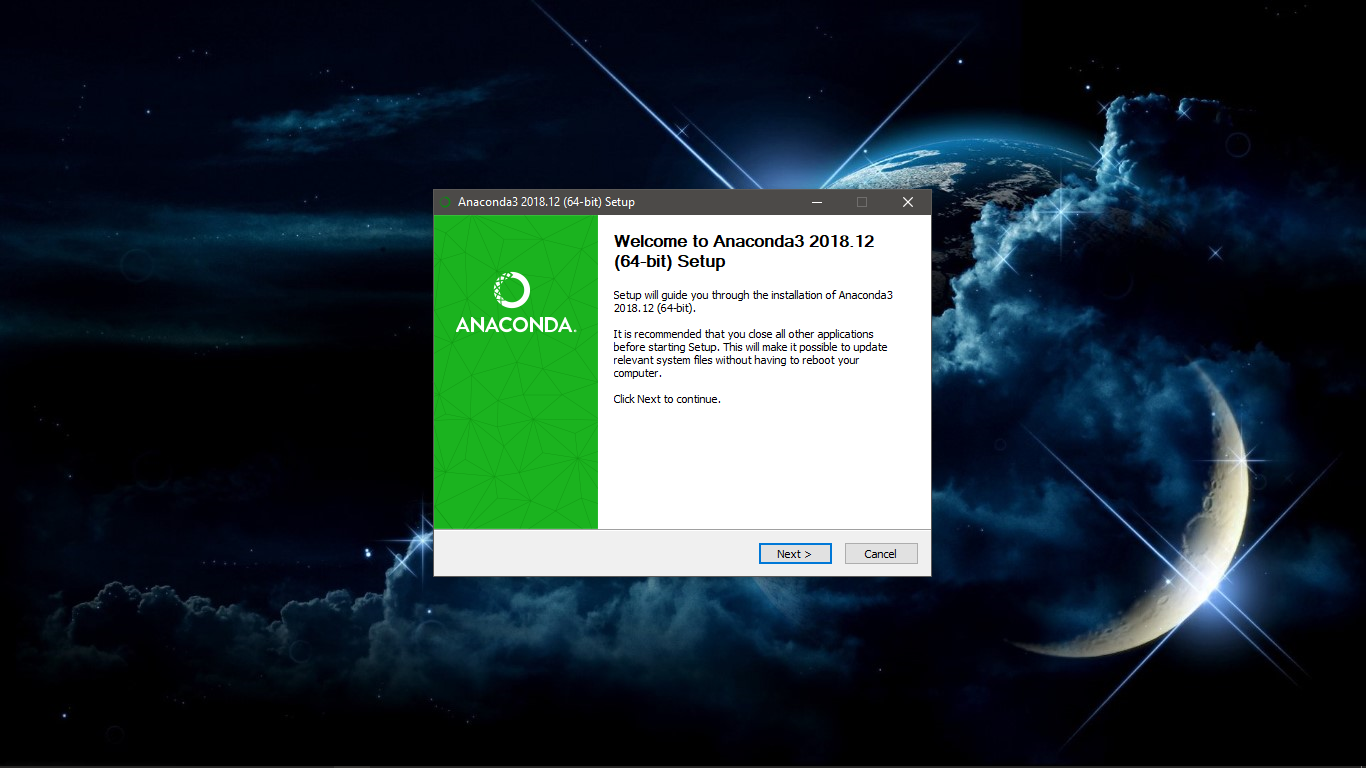
\includegraphics[width=3cm,height=3cm]{figures/Screenshot(80).png}
        \caption{Tampilan Awal}
        \label{awal}
        \end{figure}

    \item Kemudian Klik I Agree
    \begin{figure}[!htbp]
        \centering
        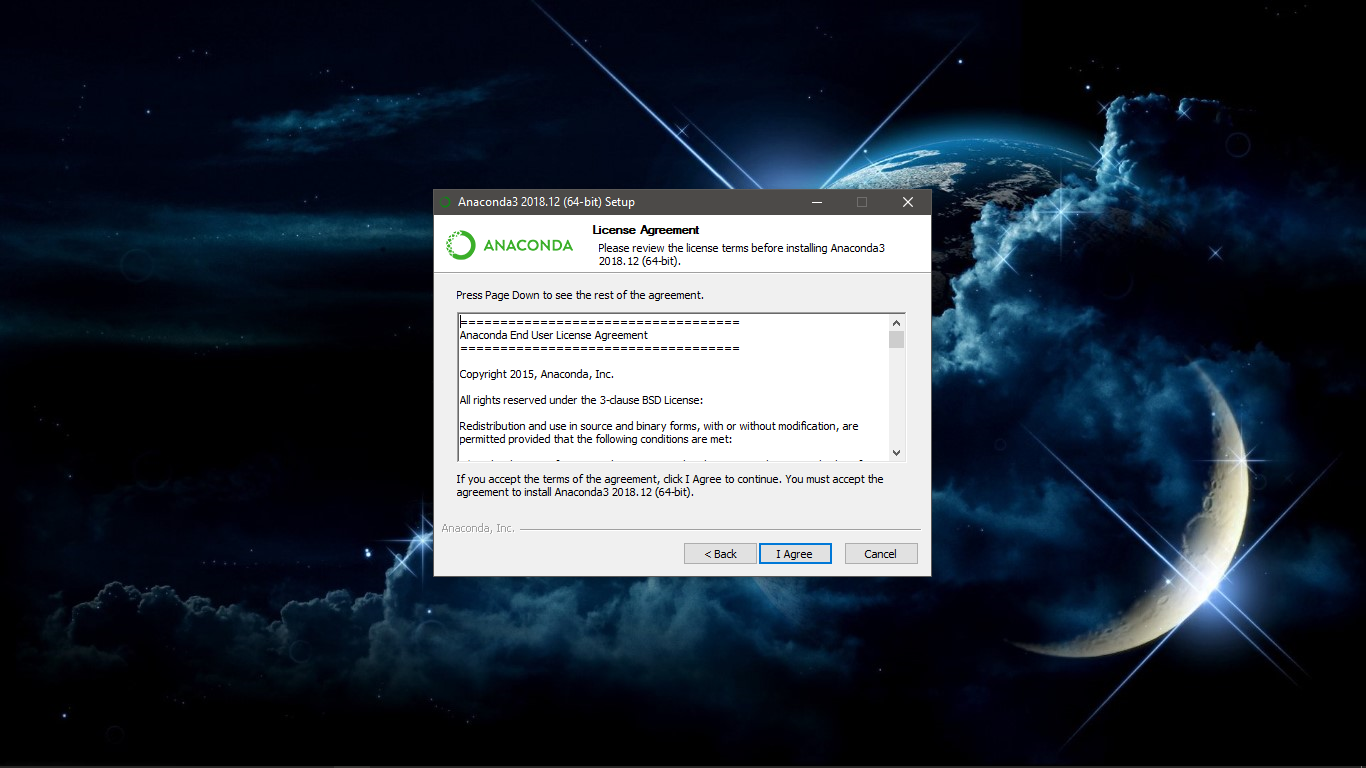
\includegraphics[width=3cm,height=3cm]{figures/Screenshot(81).png}
        \caption{License Agreement}
        \label{License}
        \end{figure}

    \item Kemudian pilih akan di instal untuk siapa, kemudian pilih next
    \begin{figure}[!htbp]
        \centering
        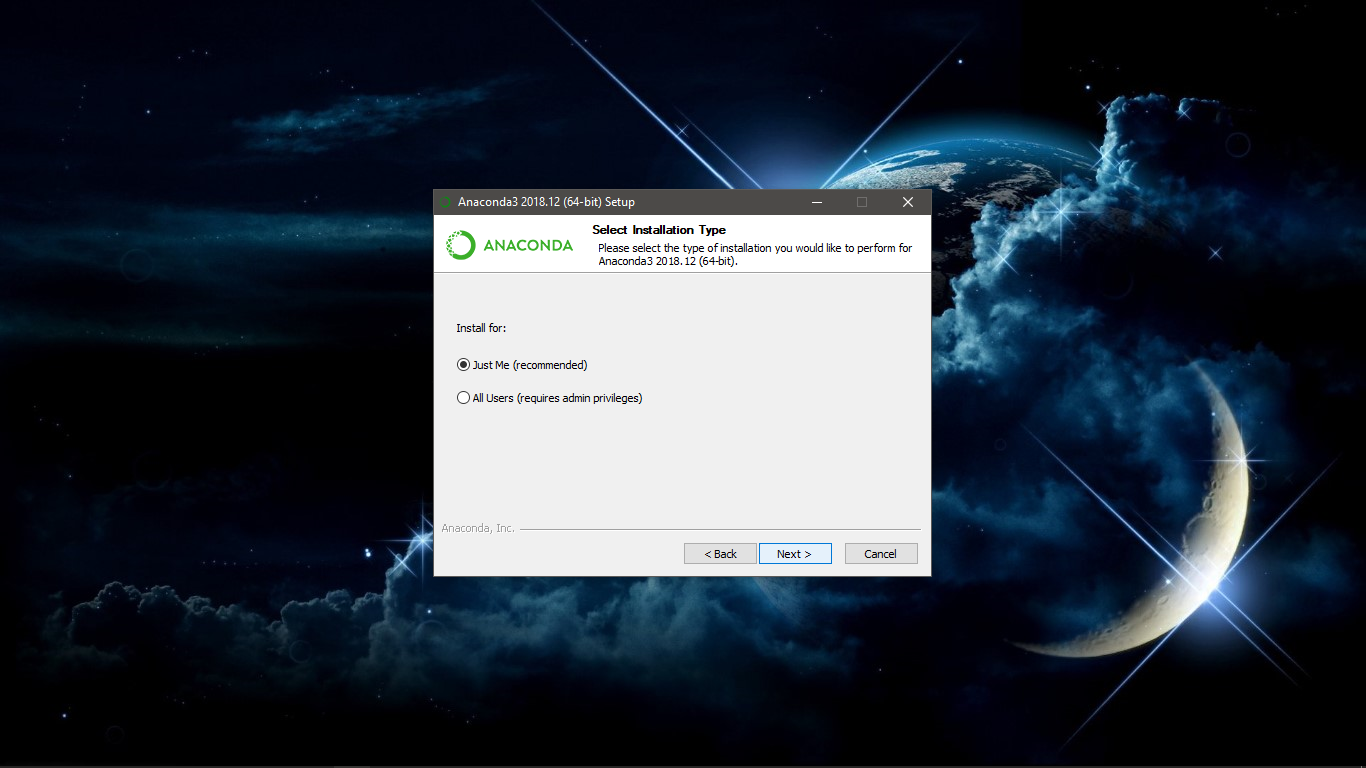
\includegraphics[width=3cm,height=3cm]{figures/Screenshot(82).png}
        \caption{Pemilihan User}
        \label{User}
        \end{figure}

    \item Kemudian tentukan dicretory nya, secara default akan berada di C:\Users\namakomputer\Anaconda3
    \begin{figure}[!htbp]
        \centering
        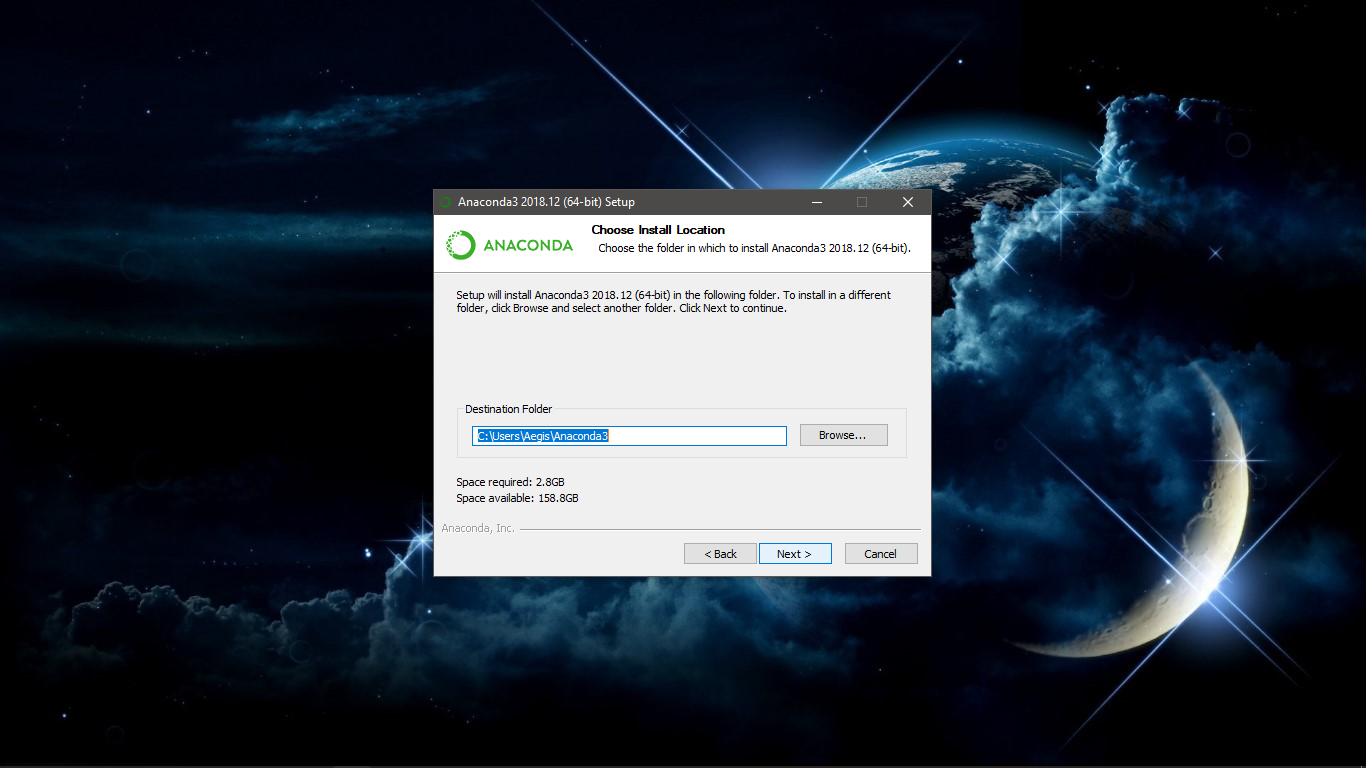
\includegraphics[width=3cm,height=3cm]{figures/Screenshot(83).png}
        \caption{Pemilihan Direktori Penyimpanan}
        \label{Directory}
        \end{figure}

    \item Kemudian Centang yang register Anaconda as default Python, Kemudian Pilih Next
    \begin{figure}[!htbp]
        \centering
        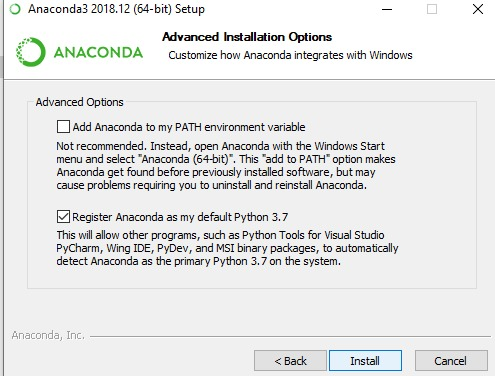
\includegraphics[width=3cm,height=3cm]{figures/Screenshot(84).jpeg}
        \caption{Pemilihan Opsi}
        \label{opsi}
        \end{figure}

    \item Tunggu Proses Instalasi hingga selesai
    \begin{figure}[!htbp]
        \centering
        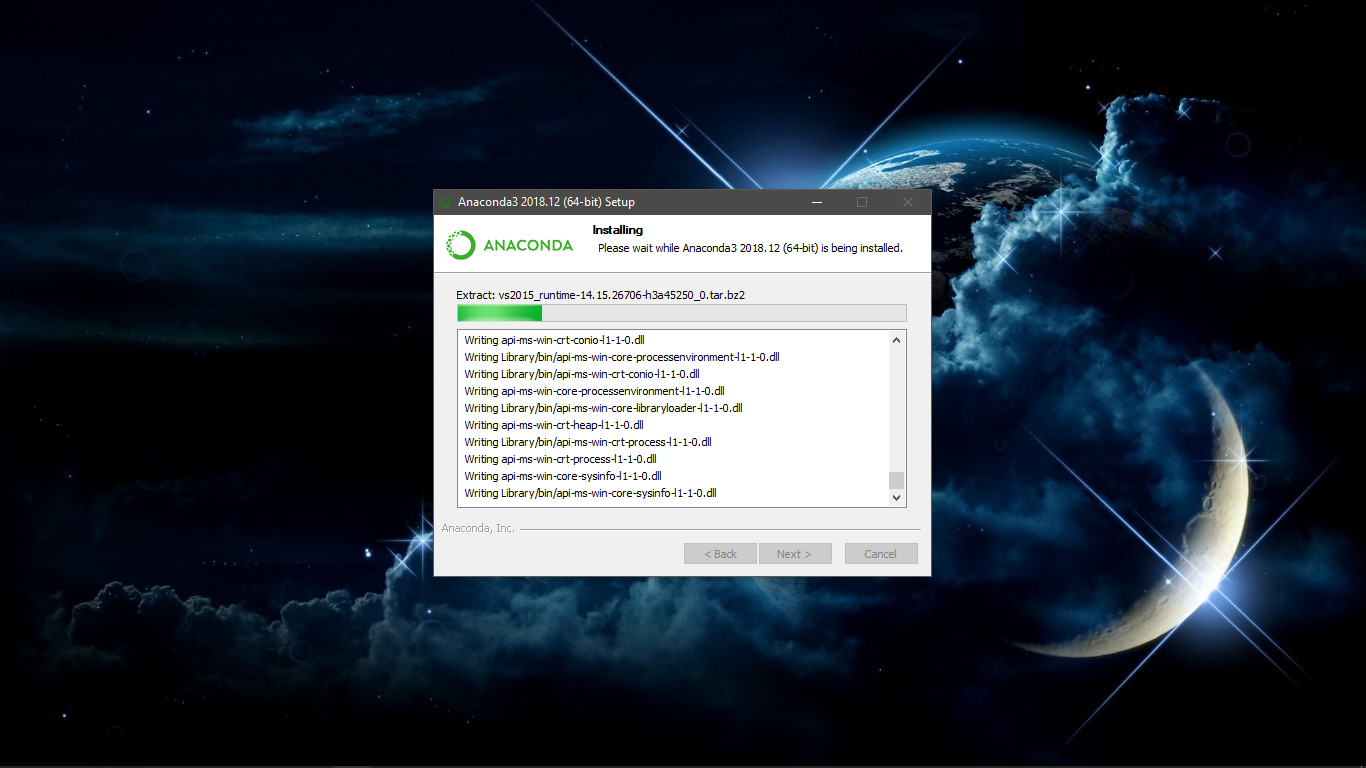
\includegraphics[width=3cm,height=3cm]{figures/Screenshot(85).png}
        \caption{Proses Instal}
        \label{Proses}
        \end{figure}

    \item Klik next
    \begin{figure}[!htbp]
        \centering
        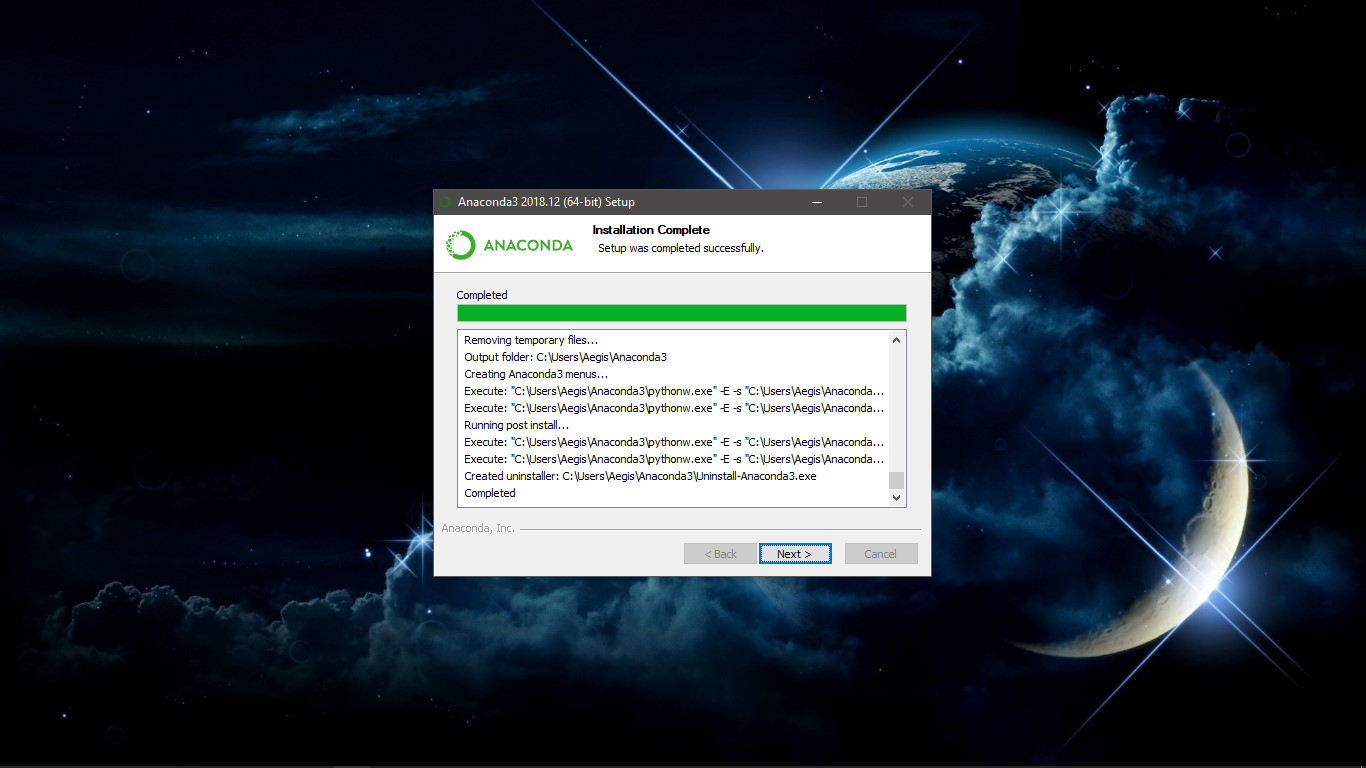
\includegraphics[width=3cm,height=3cm]{figures/Screenshot(86).png}
        \caption{Proses Instal Selesai}
        \label{Proses}
        \end{figure}

    \item kemudian jika kalian belum instal MS VSC di sarankan menginstalnya dlu, jika sudah klik skip
    \begin{figure}[!htbp]
        \centering
        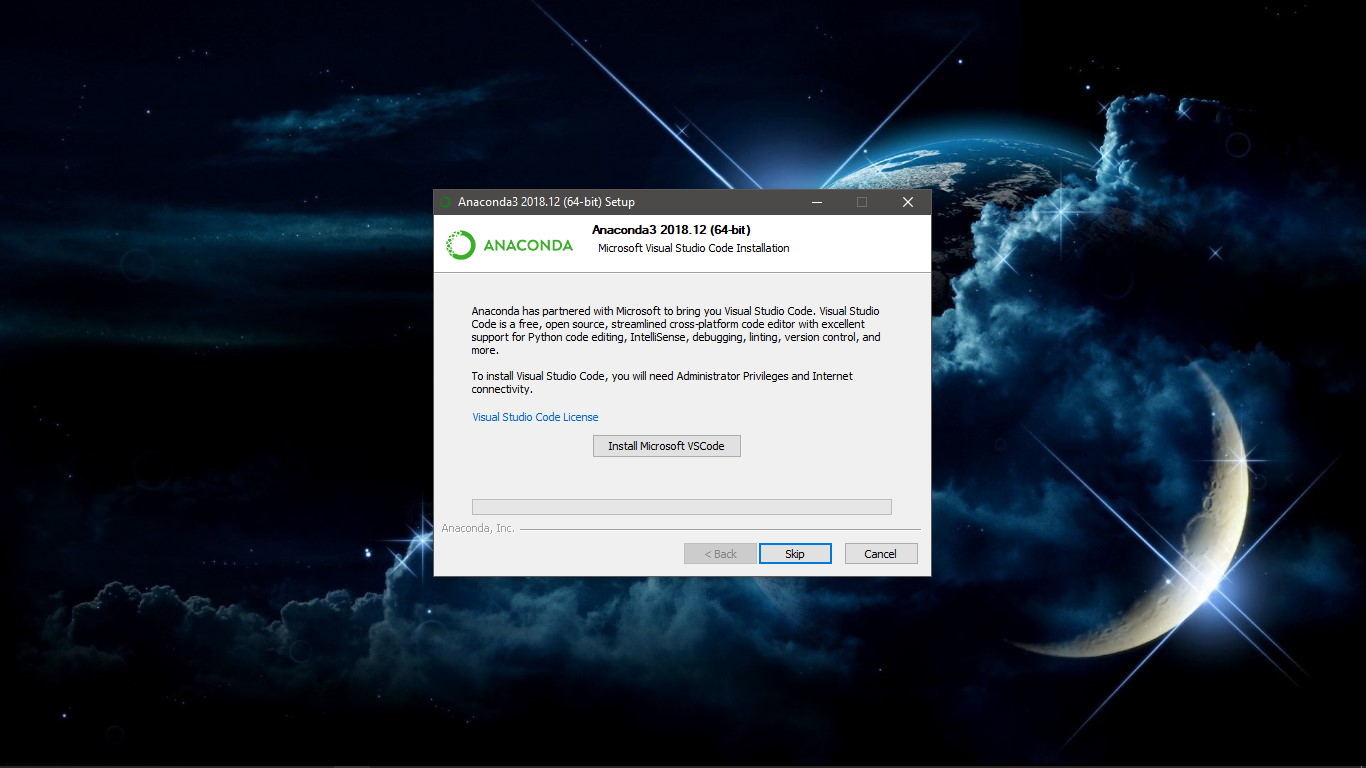
\includegraphics[width=3cm,height=3cm]{figures/Screenshot(87).png}
        \caption{Penawaran Instal MS VSC}
        \label{offering}
        \end{figure}

    \item Instalasi anaconda telah selesai
    \begin{figure}[!htbp]
        \centering
        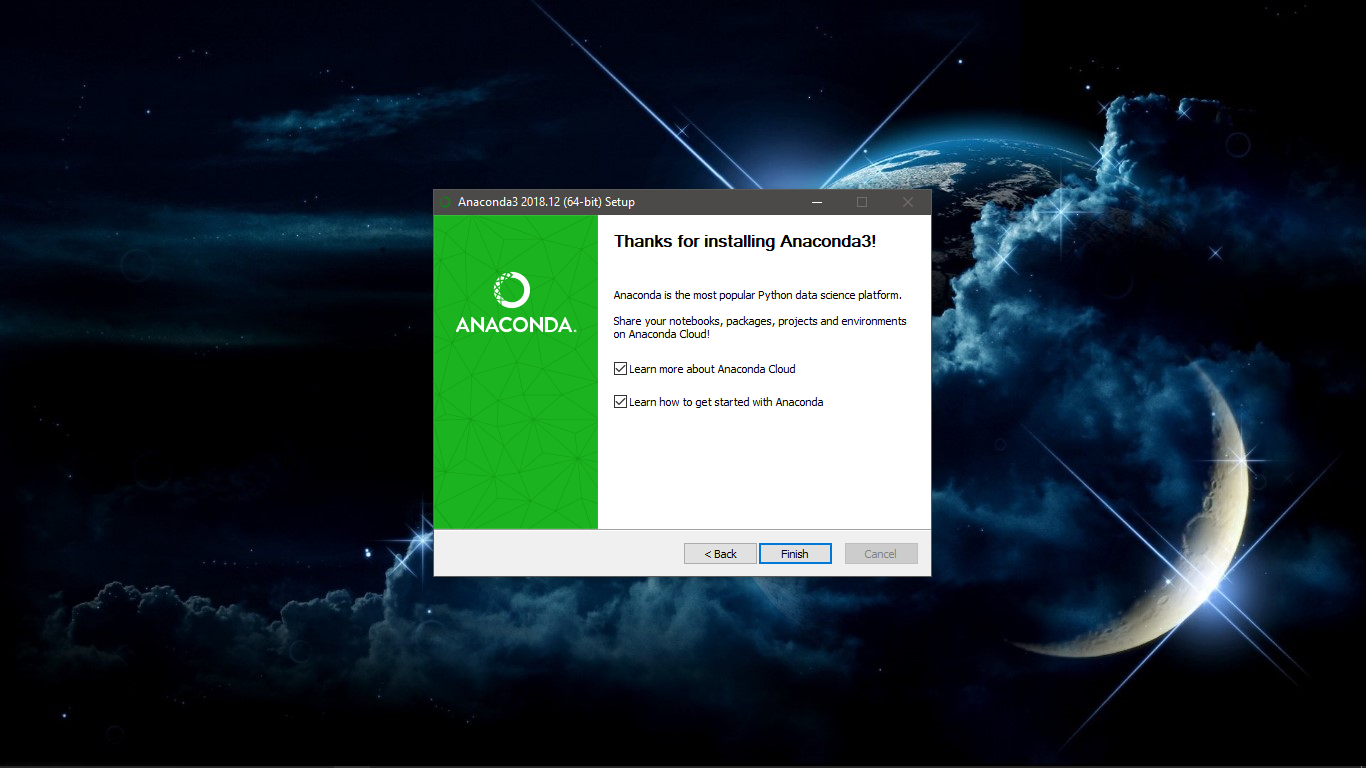
\includegraphics[width=3cm,height=3cm]{figures/Screenshot(88).png}
        \caption{Instalasi Selesai}
        \label{akhir}
        \end{figure}
\end{enumerate}
\subsection{Menggunakan Spyder}
Setelah selesai melakukan instalasi anaconda, maka ada beberapa tool yang digunakan seperti spyder

\begin{figure}[!htbp]
    \centering
    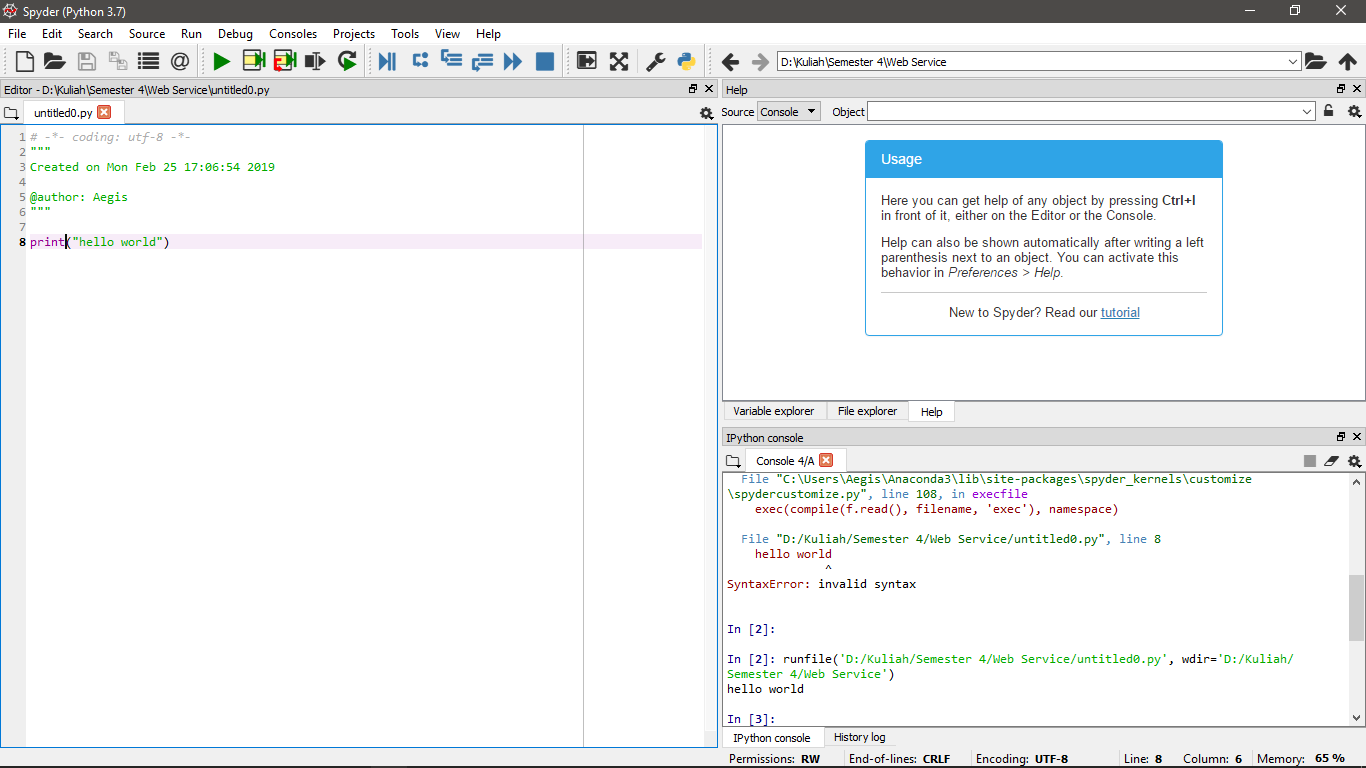
\includegraphics[width=3cm,height=3cm]{figures/Spyder.png}
    \caption{Ini adalah tampilan spyder}
    \label{spyder}
    \end{figure}

Gambar diatas menjelaskan tentang tampilan spider dan mengexsekusi program halo world.

\chapter{Judul Bagian Kedua}
%\section{Harun Ar - Rasyid}
\subsection{Teori}
\begin{enumerate}
    \item sebutkan jenis-jenis variabel dan jelaskan cara pemakaian variabel tersebut di
    kode Python
    Variabel merupakan tempat menyimpan data. Dalam phyton kita dapat membuat variable dengan cara sebagai berikut
    \lstinputlisting[firstline=74, lastline=76]{src/1174027.py}

    \item tuliskan bagaimana kode untuk meminta input dari user dan tuliskan bagaimana
    melakukan output ke layar.
    \lstinputlisting[firstline=78, lastline=79]{src/1174027.py}

    \item Tuliskan operator dasar aritmatika, tambah, kali, kurang bagi, dan bagaimana
    mengubah string ke integer dan integer ke string
    Operator  aritmatika adalah operator yang digunakan untuk melakukan perhitungan
    \lstinputlisting[firstline=81, lastline=90]{src/1174027.py}

    \item Tuliskan dan jelaskan sintak untuk perulangan, jenis-jenisnya contoh kode dan
    cara pakainya di python
    Untuk Perulangan Pada Python ada For dan While, Untuk Contohnya bisa lihat gambar berikut :
    \lstinputlisting[firstline=92, lastline=98]{src/1174027.py}

    \item Tuliskan jelaskan cara pakai sintak untuk memilih kondisi, dan bagiamana con-
    toh sintak kondisi di dalam kondisi.
    Pengambilan kondisi If yang digunakan untuk mengantisipasi kondisi yang terjadi saat program dijalankan dan menentukan tindakan apa yang akan diambil sesuai dengan kondisi.
    If statement
    \lstinputlisting[firstline=100, lastline=102]{src/1174027.py}
    
    Ifelse
    \lstinputlisting[firstline=104, lastline=107]{src/1174027.py}
    
    IfNested
    \lstinputlisting[firstline=109, lastline=114]{src/1174027.py}

    \item Tuliskan apa saja jenis error yang sering ditemui di python dalam mengerjakan
    sintak diatas. dan bagaimana cara mengatasinya
    \begin{itemize}
        \item Exception
        Kelas dasar untuk semua pengecualian / exception

        \item Stoplteration
        Dibesarkan ketika metode (iterator) berikutnya dari iterator tidak mengarah ke objek apa pun.

        \item SystemExit
        Dibesarkan oleh fungsi sys.exit ().

        \item StandardError
        Kelas dasar untuk semua pengecualian built-in kecuali StopIteration dan SystemExit.

        \item ArithmeticError
        Kelas dasar untuk semua kesalahan yang terjadi untuk perhitungan numerik.

        \item OverflowError
        Dibesarkan saat perhitungan melebihi batas maksimum untuk tipe numerik.

        \item FloatingPointError
        Dibesarkan saat perhitungan floating point gagal.

        \item ZeroDivisonError
        Dibesarkan saat pembagian atau modulo nol dilakukan untuk semua tipe numerik.

        \item AssertionError
        Dibesarkan jika terjadi kegagalan pernyataan Assert.

        \item AttributeError
        Dibesarkan jika terjadi kegagalan referensi atribut atau penugasan.
         
        \item EOFError
        Dibesarkan bila tidak ada input dari fungsi rawinput () atau input () dan akhir file tercapai.

        \item ImportError
        Dibesarkan saat sebuah pernyataan impor gagal.

        \item KeyboardInterrupt
        Dibesarkan saat pengguna menyela eksekusi program, biasanya dengan menekan Ctrl + c.

        \item LookupError
        Kelas dasar untuk semua kesalahan pencarian.

        \item IndexError
        Dibesarkan saat sebuah indeks tidak ditemukan secara berurutan.

        \item KeyError
        Dibesarkan saat kunci yang ditentukan tidak ditemukan dalam kamus.

        \item NameError
        Dibesarkan saat pengenal tidak ditemukan di namespace lokal atau global.

        \item UnboundLocalError
        Dibesarkan saat mencoba mengakses variabel lokal dalam suatu fungsi atau metode namun tidak ada nilai yang ditugaskan padanya.

        \item EnvironmentError
        Kelas dasar untuk semua pengecualian yang terjadi di luar lingkungan Python.

        \item IOError
        Dibesarkan saat operasi input / output gagal, seperti pernyataan cetak atau fungsi open () saat mencoba membuka file yang tidak ada.

        \item OSError
        Dibangkitkan untuk kesalahan terkait sistem operasi.

        \item SyntaxError
        Dibesarkan saat ada kesalahan dengan sintaks Python.

        \item IndentationError
        Dibesarkan saat indentasi tidak ditentukan dengan benar.

        \item SystemError
        Dibesarkan saat penafsir menemukan masalah internal, namun bila kesalahan ini ditemui juru bahasa Python tidak keluar.

        \item SystemExit
        Dibesarkan saat juru bahasa Python berhenti dengan menggunakan fungsi sys.exit (). Jika tidak ditangani dalam kode, menyebabkan penafsir untuk keluar.

        \item TypeError
        Dibesarkan saat operasi atau fungsi dicoba yang tidak valid untuk tipe data yang ditentukan.

        \item ValueError
        Dibesarkan ketika fungsi bawaan untuk tipe data memiliki jenis argumen yang valid, namun argumen tersebut memiliki nilai yang tidak valid yang ditentukan.

        \item RuntimeError
        Dibesarkan saat kesalahan yang dihasilkan tidak termasuk dalam kategori apa pun.

        \item NotImplementedError
        Dibesarkan ketika metode abstrak yang perlu diimplementasikan di kelas warisan sebenarnya tidak dilaksanakan.
    \end{itemize}

    \item Tuliskan dan jelaskan cara memakai Try Except.
    \lstinputlisting[firstline=116, lastline=122]{src/1174027.py}

\end{enumerate}
\subsection{Ketrampilan Pemrograman}
\begin{enumerate}
    \item Buatlah luaran huruf yang dirangkai dari tanda bintang, pagar atau plus dari
    NPM kita. Tanda bintang untuk NPM mod 3=0, tanda pagar untuk NPM mod
    3 =1, tanda plus untuk NPM mod3=2.
    \lstinputlisting[firstline=7, lastline=17]{src/1174027.py}

    \item Buatlah program hello word dengan input NPM yang disimpan dalam sebuah
    variabel string bernama NPM dan output sebanyak dua dijit belakang NPM.
    \lstinputlisting[firstline=19, lastline=24]{src/1174027.py}
    
    \item Buatlah program hello word dengan input nama yang disimpan dalam sebuah
    variabel string bernama NPM dan beri luaran output berupa tiga karakter
    belakang dari NPM sebanyak penjumlahan tiga dijit tersebut.
    \lstinputlisting[firstline=26, lastline=31]{src/1174027.py}

    \item Buatlah program hello word dengan input nama yang disimpan dalam sebuah
    variabel string bernama NPM dan beri luaran output berupa digit ketiga dari
    belakang dari variabel NPM,
    \lstinputlisting[firstline=33, lastline=35]{src/1174027.py}

    \item Buat program dengan mengisi variabel alfabet
    dengan nomor npm satu persatu berurut.
    \lstinputlisting[firstline=37, lastline=48]{src/1174027.py}

    \item Dari soal no 5, Lakukan penjumlahan dari seluruh variabel tersebut.
    \lstinputlisting[firstline=50, lastline=51]{src/1174027.py}

    \item Dari soal no 5, Lakukan perkalian dari seluruh variabel tersebut.
    \lstinputlisting[firstline=53, lastline=54]{src/1174027.py}

    \item Dari soal no 5, Lakukan print secara vertikal dari NPM anda menggunakan
    variabel diatas.
    \lstinputlisting[firstline=56, lastline=63]{src/1174027.py}

    \item Dari soal no 5, Lakukan print NPM anda tapi hanya dijit genap saja.
    \lstinputlisting[firstline=65, lastline=66]{src/1174027.py}

    \item Dari soal no 5, Lakukan print NPM anda tapi hanya dijit ganjil saja.
    \lstinputlisting[firstline=68, lastline=69]{src/1174027.py}

    \item Dari soal no 5, Lakukan print NPM anda tapi hanya dijit yang termasuk bilan-
    gan prima saja.
    \lstinputlisting[firstline=71, lastline=72]{src/1174027.py}

\end{enumerate}
\subsection{Ketrampilan Penanganan Error}
    \lstinputlisting[language=Python]{src/err2.py}
%%%%%%%%%%%%%%%%%%%%%%%%%%%%%%%%%%%%%%%%%%%%%%%%%%%%%%%%%%%%%%%%%%%%%%%%%%%%%%%%%%%%%%%%%%%%%%%%%%%%%%%%5
\section{Dwi Yulianingsih}
\subsection{Teori}
\begin{enumerate}
    \item Jenis-jenis variable phyton dan cara pemakaiannya
Variabel merupakan tempat menyimpan data. Dalam Phyton terdapat variabel biasa dan variabel array dengan berbagai type data diantaranya adalah variabel dengan type data number, string, dan boolean. Dalam phyton kita dapat membuat variable dengan cara sebagai gambar1 berikut
    \lstinputlisting[firstline=8, lastline=45]{src/teori.py}

    \item Kode untuk meminta input dari user dan bagaimana melakukan output ke layar seperti pada gambar2
    \lstinputlisting[firstline=47, lastline=49]{src/teori.py}

    \item Operator dasar aritmatika
Ada operator penambahan, pengurangan perkalian, perkalian, pembagian, modulus, perpangkatan, dan pembulatan decimal.
    \lstinputlisting[firstline=51, lastline=74]{src/teori.py}

    \item Perulangan
Terdapat dua jenis perulangan di dalam phyton yaitu perulangan while dan perulangan for
    \lstinputlisting[firstline=76, lastline=86]{src/teori.py}

    \item sintak Untuk memilih kondisi, dan kondisi didalam kondisi
Pengambilan kondisi If yang digunakan untuk mengantisipasi kondisi yang terjadi saat program dijalankan dan menentukan tindakan apa yang akan diambil sesuai dengan kondisi.
    \lstinputlisting[firstline=88, lastline=111]{src/teori.py}


    \item Jenis-jenis error pada phyton
Syntax Errors adalah keadaan dimana kode python mengalami kesalahan penulisan. 
ZeroDivisonError adalah eror yang terjadi saat eksekusi program menghasilkan perhitungan matematika pembagian dengan angka nol.
NameError adalah eror yang terjadi saat kode di eksekusi terhadap local name atau global name yang tidak terdefinisi. 
TypeError adalah eror yang terjadi saat dilakukan eksekusi pada suatu operasi atau fungsi dengan type object yang tidak sesuai.

    \item Cara memakai try except
Cara pemakaian try except adalah sebagai berikut :
    \lstinputlisting[firstline=113, lastline=117]{src/teori.py}


\end{enumerate}

\subsection{praktek}
\begin{enumerate}
    \item Jawaban soal no 1
    \lstinputlisting[firstline=7, lastline=17]{src/1174009.py}
    \item Jawaban soal no 2
    \lstinputlisting[firstline=19, lastline=24]{src/1174009.py}
    \item Jawaban soal no 3
    \lstinputlisting[firstline=26, lastline=31]{src/1174009.py}
    \item Jawaban soal no 4
    \lstinputlisting[firstline=33, lastline=35]{src/1174009.py}
    \item Jawaban soal no 5
    \lstinputlisting[firstline=37, lastline=48]{src/1174009.py}
    \item Jawaban soal no 6
    \lstinputlisting[firstline=50, lastline=51]{src/1174009.py}
    \item Jawaban soal no 7
    \lstinputlisting[firstline=53, lastline=54]{src/1174009.py}
    \item Jawaban soal no 8
    \lstinputlisting[firstline=56, lastline=63]{src/1174009.py}
    \item Jawaban soal no 9
    \lstinputlisting[firstline=65, lastline=66]{src/1174009.py}
    \item Jawaban soal no 10
    \lstinputlisting[firstline=68, lastline=69]{src/1174009.py}
    \item Jawaban soal no 11
    \lstinputlisting[firstline=71, lastline=72]{src/1174009.py}
\end{enumerate}

\subsection{Keterampilan dan penanganan eror}
    \lstinputlisting[firstline=8, lastline=15]{src/eror.py}

%%%%%%%%%%%%%%%%%%%%%%%%%%%%%%%%%%%%%%%%%%%%%%%%%%%%%%%%%%

\section{Kadek Diva Krishna Murti}

\subsection{Teori}

\begin{enumerate}
\item Jenis-jenis variabel dan cara pemakaiannya di Python.

\begin{enumerate}
\item Boolean
\lstinputlisting[caption=Contoh kode penggunaan Boolean., firstline=1, lastline=3]{src/1174006.py}

\item String
\lstinputlisting[caption=Contoh kode penggunaan String., firstline=5, lastline=7]{src/1174006.py}

\item Integer
\lstinputlisting[caption=Contoh kode penggunaan Integer., firstline=9, lastline=11]{src/1174006.py}

\item Float
\lstinputlisting[caption=Contoh kode penggunaan Float., firstline=13, lastline=15]{src/1174006.py}

\item Hexadecimal
\lstinputlisting[caption=Contoh kode penggunaan Hexadecimal., firstline=17, lastline=19]{src/1174006.py}

\item Complex
\lstinputlisting[caption=Contoh kode penggunaan Complex., firstline=21, lastline=23]{src/1174006.py}

\item List
\lstinputlisting[caption=Contoh kode penggunaan List., firstline=25, lastline=28]{src/1174006.py}

\item Tuple
\lstinputlisting[caption=Contoh kode penggunaan Tuple., firstline=30, lastline=33]{src/1174006.py}

\item Set
\lstinputlisting[caption=Contoh kode penggunaan Set., firstline=35, lastline=37]{src/1174006.py}

\item Dictionary
\lstinputlisting[caption=Contoh kode penggunaan Dictionary., firstline=40, lastline=43]{src/1174006.py}

\end{enumerate}

\item Kode untuk meminta input dan melakukan output di Python.
\lstinputlisting[caption=Contoh kode input dan output., firstline=45, lastline=48]{src/1174006.py}

\item Operator dasar aritmatika dan mengubah tipe data di Python.

Operator dasar aritmatika
\begin{enumerate}
\item Pertambahan
Operator ini dipergunakan untuk melakukan operasi pertambahan.
\lstinputlisting[caption=Contoh kode operasi pertambahan., firstline=51, lastline=55]{src/1174006.py}
\item Pengurangan
Operator ini dipergunakan untuk melakukan operasi pengurangan.
\lstinputlisting[caption=Contoh kode operasi pengurangan., firstline=57, lastline=61]{src/1174006.py}
\item Perkalian
Operator ini dipergunakan untuk melakukan operasi perkalian.
\lstinputlisting[caption=Contoh kode operasi perkalian., firstline=63, lastline=67]{src/1174006.py}
\item Pembagian
Operator ini dipergunakan untuk melakukan operasi pembagian.
\lstinputlisting[caption=Contoh kode operasi pembagian., firstline=69, lastline=73]{src/1174006.py}
\item Modulus
Operator ini dipergunakan untuk melakukan operasi modulus.
\lstinputlisting[caption=Contoh kode operasi modulus., firstline=75, lastline=79]{src/1174006.py}
\item Perpangkatan
Operator ini dipergunakan untuk melakukan operasi perpangkatan.
\lstinputlisting[caption=Contoh kode operasi perpangkatan., firstline=81, lastline=85]{src/1174006.py}
\item Pembulatan Hasil Bagi
Operator ini dipergunakan untuk melakukan operasi pembulatan hasil bagi.
\lstinputlisting[caption=Contoh kode operasi pembulatan hasil bagi., firstline=87, lastline=91]{src/1174006.py}
\end{enumerate}

Mengubah tipe data
\begin{enumerate}
\item String ke Integer
\lstinputlisting[caption=Contoh kode konversi string ke integer., firstline=94, lastline=97]{src/1174006.py}
\item Integer ke String
\lstinputlisting[caption=Contoh kode konversi integer ke string., firstline=100, lastline=102]{src/1174006.py}
\end{enumerate}


\item Sintak perulangan, jenis-jenisnya, dan cara penggunaannya di Python.
\begin{enumerate}
\item While Loop
While Loop adalah perulangan yang mengeksekusi statement berkali-kali selama kondisi bernilai benar atau True.
\lstinputlisting[caption=Contoh kode penggunaan while loop., firstline=104, lastline=108]{src/1174006.py}

\item For Loop
For Loop  adalah perualangan yang mengulangi item dari urutan apapun, seperti list atau string.
\lstinputlisting[caption=Contoh kode penggunaan for loop., firstline=110, lastline=113]{src/1174006.py}

\item Nested Loop
Nested Loop merupakan perulangan yang berada di perulangan atau biasa disebut dengan perulangan bersarang.
\lstinputlisting[caption=Contoh kode penggunaan nested loop., firstline=115, lastline=122]{src/1174006.py}

\end{enumerate}

\item Sintak pengkodisian dan contoh penggunaannya kondisi di dalam kondisi di Python.
\begin{enumerate}
\item If
Kondisi ini dipergunakan jika penkondisiannya hanya satu.
\lstinputlisting[caption=Contoh kode penggunaan if., firstline=124, lastline=127]{src/1174006.py}

\item If Else
Kondisi ini dipergunakan jika pengkondisiannya ada dua.
\lstinputlisting[caption=Contoh kode penggunaan if else., firstline=129, lastline=134]{src/1174006.py}

\item Elif
Kondisi ini dipergunakan jika pengkondisiannya lebih dari dua.
\lstinputlisting[caption=Contoh kode penggunaan elif., firstline=136, lastline=143]{src/1174006.py}

\item Kondisi di dalam kondisi
Kondisi ini dipergunakan jika pengkondisiannya memerlukan pengkondisian di dalamnya.
\lstinputlisting[caption=Contoh kode penggunaan kondisi di dalam kondisi., firstline=146, lastline=156]{src/1174006.py}

\end{enumerate}

\item Jenis-jenis error dan cara mengatasinya di Python.
\begin{itemize}
\item Syntax Errors
Syntax Errors adalah suatu keadaan saat kode python mengalami kesalahan penulisan. Solusinya adalah memperbaiki penulisan kode yang salah.

\item Zero Division Error
ZeroDivisonError adalah exceptions yang terjadi saat eksekusi program menghasilkan perhitungan matematika pembagian dengan angka nol (0). Solusinya adalah tidak membagi suatu yang hasilnya nol.

\item Name Error
NameError adalah exception yang terjadi saat kode melakukan eksekusi terhadap local name atau global name yang tidak terdefinisi. Solusinya adalah memastikan variabel atau function yang dipanggil ada atau tidak salah ketik.

\item Type Error
TypeError adalah exception yang terjadi saat dilakukan eksekusi terhadap suatu operasi atau fungsi dengan type object yang tidak sesuai. Solusinya adalah mengkoversi varibelnya sesuai dengan tipe data yang akan digunakan.

\end{itemize}

\item Cara pemakaian Try Except di Python.
Berikut ini adalah contoh penggunaan try except.
\lstinputlisting[caption=Contoh kode penggunaan try except., firstline=158, lastline=164]{src/1174006.py}

\end{enumerate}
\hfill \break

\subsection{Ketrampilan Pemrograman}

\begin{enumerate}
\item Jawaban Soal 1
\lstinputlisting[firstline=166, lastline=176]{src/1174006.py}

\item Jawaban Soal 2
\lstinputlisting[firstline=178, lastline=184]{src/1174006.py}

\item Jawaban Soal 3
\lstinputlisting[firstline=186, lastline=192]{src/1174006.py}

\item Jawaban Soal 4
\lstinputlisting[firstline=194, lastline=197]{src/1174006.py}

\item Jawaban Soal 5
\lstinputlisting[firstline=199, lastline=212]{src/1174006.py}

\item Jawaban Soal 6
\lstinputlisting[firstline=215, lastline=217]{src/1174006.py}

\item Jawaban Soal 7
\lstinputlisting[firstline=219, lastline=221]{src/1174006.py}

\item Jawaban Soal 8
\lstinputlisting[firstline=223, lastline=226]{src/1174006.py}

\item Jawaban Soal 9
\lstinputlisting[firstline=228, lastline=233]{src/1174006.py}

\item Jawaban Soal 10
\lstinputlisting[firstline=236, lastline=240]{src/1174006.py}

\item Jawaban Soal 11
\lstinputlisting[firstline=243, lastline=245]{src/1174006.py}

\end{enumerate}
\hfill \break

\subsection{Ketrampilan Penanganan Error}
\begin{enumerate}
\item Jawaban Soal No. 1
\begin{itemize}
\item Syntax Errors
Syntax Errors adalah suatu keadaan saat kode python mengalami kesalahan penulisan. Solusinya adalah memperbaiki penulisan kode yang salah.

\item Zero Division Error
ZeroDivisonError adalah exceptions yang terjadi saat eksekusi program menghasilkan perhitungan matematika pembagian dengan angka nol (0). Solusinya adalah tidak membagi suatu yang hasilnya nol.

\item Name Error
NameError adalah exception yang terjadi saat kode melakukan eksekusi terhadap local name atau global name yang tidak terdefinisi. Solusinya adalah memastikan variabel atau function yang dipanggil ada atau tidak salah ketik.

\item Type Error
TypeError adalah exception yang terjadi saat dilakukan eksekusi terhadap suatu operasi atau fungsi dengan type object yang tidak sesuai. Solusinya adalah mengkoversi varibelnya sesuai dengan tipe data yang akan digunakan.

\end{itemize}

\item Jawaban Soal No. 2																			
\lstinputlisting[firstline=1, lastline=7]{src/2err_1174006.py}
\end{enumerate}
 
 %%%%%%%%%%%%%%%%%%%%%%%%%%%%%%%%%%%%%%%%%%%%%%%%%%%%%%%%%%%%%%%%
 \section{Dezha Aidil Martha}
\subsection{Teori}
\begin{enumerate}
	\item Jenis-jenis variable phyton dan cara pemakaiannya
Variabel merupakan tempat menyimpan data. Dalam Phyton terdapat beberapa variabel dengan berbagai type data diantaranya adalah variabel dengan type data number, string, dan boolean. Dalam phyton kita dapat membuat variable dengan cara sebagai gambar berikut
   \lstinputlisting[firstline=8, lastline=12]{src/1174025_teori.py}
	\item Kode untuk meminta input dari user dan bagaimana melakukan output ke layar
 \lstinputlisting[firstline=67, lastline=68]{src/1174025_teori.py}
	\item Operator dasar aritmatika
Ada operator penambahan, pengurangan perkalian, perkalian, pembagian, modulus, perpangkatan, dan pembulatan decimal.
\lstinputlisting[firstline=71, lastline=94]{src/1174025_teori.py}
	\item Perulangan
Terdapat dua jenis perulangan di dalam phyton yaitu perulangan while dan perulangan for
 \lstinputlisting[firstline=97, lastline=99]{src/1174025_teori.py}
 \lstinputlisting[firstline=102, lastline=105]{src/1174025_teori.py}
	\item sintak Untuk memilih kondisi, dan kondisi didalam kondisi
Pengambilan kondisi If yang digunakan untuk mengantisipasi kondisi yang terjadi saat program dijalankan dan menentukan tindakan apa yang akan diambil sesuai dengan kondisi.
  \lstinputlisting[firstline=108, lastline=111]{src/1174025_teori.py}
  \lstinputlisting[firstline=114, lastline=119]{src/1174025_teori.py}
  \lstinputlisting[firstline=122, lastline=129]{src/1174025_teori.py}

	\item Jenis-jenis error pada phyton
Syntax Errors adalah keadaan dimana kode python mengalami kesalahan penulisan. 
ZeroDivisonError adalah eror yang terjadi saat eksekusi program menghasilkan perhitungan matematika pembagian dengan angka nol.
NameError adalah eror yang terjadi saat kode di eksekusi terhadap local name atau global name yang tidak terdefinisi. 
TypeError adalah eror yang terjadi saat dilakukan eksekusi pada suatu operasi atau fungsi dengan type object yang tidak sesuai.

	\item Cara memakai try except
Cara pemakaian try except adalah sebagai berikut :
\lstinputlisting[firstline=132, lastline=138]{src/1174025_teori.py}

\end{enumerate}

\subsection{praktek}
\begin{enumerate}
	\item Jawaban soal no 1
	\lstinputlisting[firstline=11, lastline=20]{src/1174025_praktek.py}
	\item Jawaban soal no 2
	\lstinputlisting[firstline=24, lastline=28]{src/1174025_praktek.py}
	\item Jawaban soal no 3
	\lstinputlisting[firstline=33, lastline=37]{src/1174025_praktek.py}
	\item Jawaban soal no 4
	\lstinputlisting[firstline=40, lastline=41]{src/1174025_praktek.py}
	\item Jawaban soal no 5
	\lstinputlisting[firstline=44, lastline=56]{src/1174025_praktek.py}
	\item Jawaban soal no 6
	\lstinputlisting[firstline=59, lastline=60]{src/1174025_praktek.py}
	\item Jawaban soal no 7
	\lstinputlisting[firstline=63, lastline=64]{src/1174025_praktek.py}
	\item Jawaban soal no 8
	\lstinputlisting[firstline=67, lastline=71]{src/1174025_praktek.py}
	\item Jawaban soal no 9
	\lstinputlisting[firstline=74, lastline=74]{src/1174025_praktek.py}
	\item Jawaban soal no 10
	\lstinputlisting[firstline=77, lastline=77]{src/1174025_praktek.py}
	\item Jawaban soal no 11
	\lstinputlisting[firstline=80, lastline=80]{src/1174025_praktek.py}
\end{enumerate}

\subsection{Keterampilan dan penanganan eror}
	\lstinputlisting[firstline=10, lastline=17]{src/erro2.py}
%%%%%%%%%%%%%%%%%%%%%%%%%%%%%%%%%%%%%%%%%%%%%%%%%%%%%%%%%%%%%%%%
 \section{Evietania Charis Sujadi}
\subsection{Teori}
\begin{enumerate}
    \item Jenis jenis variable phyton dan cara pemakaiannya
Variabel merupakan tempat menyimpan data. Dalam Phyton terdapat beberapa variabel dengan berbagai type data diantaranya adalah variabel dengan type data number, string, dan boolean. Dalam phyton kita dapat membuat variable dengan cara sebagai gambar berikut
   \lstinputlisting[firstline=8, lastline=12]{src/1174051_teori.py}
    \item Kode untuk meminta input dari user dan bagaimana melakukan output ke layar
 \lstinputlisting[firstline=67, lastline=68]{src/1174051_teori.py}
    \item Operator dasar aritmatika
Ada operator penambahan, pengurangan perkalian, perkalian, pembagian, modulus, perpangkatan, dan pembulatan decimal.
\lstinputlisting[firstline=71, lastline=94]{src/1174051_teori.py}
    \item Perulangan
Terdapat dua jenis perulangan di dalam phyton yaitu perulangan while dan perulangan for
 \lstinputlisting[firstline=97, lastline=99]{src/1174051_teori.py}
 \lstinputlisting[firstline=102, lastline=105]{src/1174051_teori.py}
    \item sintak Untuk memilih kondisi, dan kondisi didalam kondisi
Pengambilan kondisi If yang digunakan untuk mengantisipasi kondisi yang terjadi saat program dijalankan dan menentukan tindakan apa yang akan diambil sesuai dengan kondisi.
  \lstinputlisting[firstline=108, lastline=111]{src/1174051_teori.py}
  \lstinputlisting[firstline=114, lastline=119]{src/1174051_teori.py}
  \lstinputlisting[firstline=122, lastline=129]{src/1174051_teori.py}

    \item Jenis-jenis error pada phyton
Syntax Errors adalah keadaan dimana kode python mengalami kesalahan penulisan. 
ZeroDivisonError adalah eror yang terjadi saat eksekusi program menghasilkan perhitungan matematika pembagian dengan angka nol.
NameError adalah eror yang terjadi saat kode di eksekusi terhadap local name atau global name yang tidak terdefinisi. 
TypeError adalah eror yang terjadi saat dilakukan eksekusi pada suatu operasi atau fungsi dengan type object yang tidak sesuai.

    \item Cara memakai try except
Cara pemakaian try except adalah sebagai berikut :
\lstinputlisting[firstline=132, lastline=138]{src/1174051_teori.py}

\end{enumerate}

\subsection{praktek}
\begin{enumerate}
    \item Jawaban soal no 1
    \lstinputlisting[firstline=11, lastline=20]{src/1174051_praktek.py}
    \item Jawaban soal no 2
    \lstinputlisting[firstline=24, lastline=28]{src/1174051_praktek.py}
    \item Jawaban soal no 3
    \lstinputlisting[firstline=33, lastline=37]{src/1174051_praktek.py}
    \item Jawaban soal no 4
    \lstinputlisting[firstline=40, lastline=41]{src/1174051_praktek.py}
    \item Jawaban soal no 5
    \lstinputlisting[firstline=44, lastline=56]{src/1174051_praktek.py}
    \item Jawaban soal no 6
    \lstinputlisting[firstline=59, lastline=60]{src/1174051_praktek.py}
    \item Jawaban soal no 7
    \lstinputlisting[firstline=63, lastline=64]{src/1174051_praktek.py}
    \item Jawaban soal no 8
    \lstinputlisting[firstline=67, lastline=71]{src/1174051_praktek.py}
    \item Jawaban soal no 9
    \lstinputlisting[firstline=74, lastline=74]{src/1174051_praktek.py}
    \item Jawaban soal no 10
    \lstinputlisting[firstline=77, lastline=77]{src/1174051_praktek.py}
    \item Jawaban soal no 11
    \lstinputlisting[firstline=80, lastline=80]{src/1174051_praktek.py}
\end{enumerate}

\subsection{Keterampilan dan penanganan eror}
    \lstinputlisting[firstline=10, lastline=17]{src/ror.py}
%%%%%%%%%%%%%%%%%%%%%%%%%%%%%%%%%%%%%%%%%%%%%%%%%%%%%%%%%%%%%%%%%%%%%%%%%%%%%%%%%%%%%%%%%%%%%%%%%%%%%%%%%%%%%%
\section{Perintah Navigasi}
Perintah navigasi direktori
\section{Damara Benedikta}
\subsection{Teori}
\begin{enumerate}
	\item jenis-jenis variable phyton dan cara pemakaiannya
Variable merupakan tempat untuk menyimpan data, Isi dari variabel itu dapat berubah atau mutable sesuai dengan operasi yang diinginkan. Saat program dieksekusi maka variabellah yang bertugas menyimpan data. Dimana didalam phyton terdapat beberapa variable diantaranya number, boolean,string. Dalam membuat variabel Pythoncaranya adalah sebagai berikut
    \lstinputlisting[firstline=8,lastline=46]{src/teori1.py}
    \item operator dasar aritmatika 
dimana terdapat penjumlahan,pengurangan,pembagian,perkalian,perpangkatan,pembulatan nominal
    \lstinputlisting[firstline=47,lastline=75]{src/teori1.py}
    \item Perulangan
dalam phyton terdapat perulangan while dan for
    \lstinputlisting[firstline=76,lastline=87]{src/teori1.py}
    \item Dimana terdapat sintak untuk meilih kondisi didalam kondisi
Untuk memilih keputusan menggunakan (kondisi if) dimana digunakan untuk mengantisipasi kondisi yang terjadi saat jalannya suatu program dan menentukan tindakan apa yang akan dilakukan sesuai dengan kondisi.
    \lstinputlisting[firstline=88,lastline=112]{src/teori1.py}

    \item Jenis-jenis sintak error pada phyton
 Syntax errors Jika dalam program terdapat kesalahan sintaks maka proses akan berhenti dan menampilkan pesan kesalahan.
Runtime errors, disebut begitu karenakesalahan tidak akan muncul sampai Anda menjalankan program tersebut.Kesalahan ini juga dikenal dengan exceptions atau pengecualian karena biasanya mengindikasikan sesuatu pengecualian yang buruk telah terjadi.

Type eror merupakan eror yang terjadi saat dilakukan eksekusi pada suatu operasi dengan type object yang tidak sesuai.
ZeroDivision eror merupakan eror yang terjadi saat eksekusi program menghasilkan perhitungan matematika dengan angka 0

 \item Try except
cara memakai try except adalah sebagai berikut
    \lstinputlisting[firstline=8,lastline=17]{src/teori1.py}
    \end{enumerate}
\subsection{praktek}
\begin{enumerate}
	\item Jawaban soal no 1
	\lstinputlisting[firstline=8,lastline=17]{src/1174012.py}
	\item Jawaban soal no 2
	\lstinputlisting[firstline=18,lastline=23]{src/1174012.py}
	\item Jawaban soal no 3
	\lstinputlisting[firstline=24,lastline=29]{src/1174012.py}
	\item Jawaban soal no 4
	\lstinputlisting[firstline=30,lastline=32]{src/1174012.py}
	\item Jawaban soal no 5
	\lstinputlisting[firstline=33,lastline=43]{src/1174012.py}
	\item Jawaban soal no 6
	\lstinputlisting[firstline=44,lastline=45]{src/1174012.py}
	\item Jawaban soal no 7
	\lstinputlisting[firstline=46,lastline=47]{src/1174012.py}
	\item Jawaban soal no 8
	\lstinputlisting[firstline=48,lastline=55]{src/1174012.py}
	\item Jawaban soal no 9
	\lstinputlisting[firstline=56,lastline=57]{src/1174012.py}
	\item Jawaban soal no 10
	\lstinputlisting[firstline=58,lastline=59]{src/1174012.py}
	\item Jawaban soal no 11
	\lstinputlisting[firstline=60,lastline=61]{src/1174012.py}
\end{enumerate}

\subsection{Keterangan dan Penanganan eror}
\lstinputlisting[firstline=5,lastline=15]{src/error1.py}



\chapter{Judul Bagian Ketiga}
%%%%%%%%%%%%%%%%%%%%%%%%%%%%%%%%%%%%%%%%%%%%%%%%%%%%%%%%%%%%%%%
\section{Harun Ar - Rasyid}
\subsubsection{Pemahanan Teori}
\begin{enumerate}
    \item Apa itu fungsi, inputan fungsi dan kembalian fungsi dengan contoh kode program
    lainnya.
    Fungsi adalah bagian dari program yang dapat digunakan ulang.
    Berikut merupakan contoh fungsi dan cara pemanggilannya
    \lstinputlisting[firstline=124, lastline=127]{src/1174027.py}

    Fungsi dapat membaca parameter, parameter adalah nilai yang disediakan kepada fungsi, dimana nilai ini akan menentukan output yang akan dihasilkan fungsi.
    \lstinputlisting[firstline=129, lastline=132]{src/1174027.py}

    Statemen return digunakan untuk keluar dari fungsi. Kita juga dapat menspesifikasikan nilai kembalian.
    \lstinputlisting[firstline=134, lastline=141]{src/1174027.py}

    \item Apa itu paket dan cara pemanggilan paket atau library dengan contoh kode
    program lainnya.
    Untuk memudahkan dalam pemanggilan fungsi yang di butuhkan, agar dapat dipanggil berulang.
    Cara pemanggilannya
    \lstinputlisting[firstline=143, lastline=144]{src/1174027.py}

    \item Jelaskan Apa itu kelas, apa itu objek, apa itu atribut, apa itu method dan
    contoh kode program lainnya masing-masing.
    kelas merupakan sebuah blueprint yang mepresentasikan objek.
    objek adalah hasil cetakan dadri sebuah kelas.
    method adalah suatu upaya yang digunakan oleh object.
    \lstinputlisting[firstline=146, lastline=168]{src/1174027.py}

    \item Jelaskan cara pemanggikan library kelas dari instansiasi dan pemakaiannya den-
    gan contoh program lainnya.
    Cara Pemanggilanya 
    \begin{itemize}
        \item pertama import terlebih dahulu filenya.
        \item kemudian buat variabel untuk menampung datanya
        \item setelah itu panggil nama classnya dan panggil methodnya
        \item Gunakan perintah print untuk menampilkan hasilnya

    \end{itemize}
    \lstinputlisting[firstline=170, lastline=175]{src/1174027.py}

    \item Jelaskan dengan contoh pemakaian paket dengan perintah from kalkulator im-
    port Penambahan disertai dengan contoh kode lainnya.
    Penggunaan paket from namafile import, itu berfungsi untuk memanggil file dan fungsinya
    \lstinputlisting[firstline=143, lastline=144]{src/1174027.py}

    \item Jelaskan dengan contoh kodenya, pemakaian paket fungsi apabila le library
    ada di dalam folder.
    Pemakaian paket adalah perkumpulan fungsi-fungsi. contoh kodenya adalah sebagai berikut :

    \item Jelaskan dengan contoh kodenya, pemakaian paket kelas apabila le library ada
    di dalam folder.
    \lstinputlisting[firstline=184, lastline=184]{src/1174027.py}

\end{enumerate}
\subsubsection{Ketrampilan Pemrograman}
\begin{enumerate}
    \item Buatlah fungsi dengan inputan variabel NPM, dan melakukan print luaran huruf
    yang dirangkai dari tanda bintang, pagar atau plus dari NPM kita. Tanda
    bintang untuk NPM mod 3=0, tanda pagar untuk NPM mod 3 =1, tanda plus
    untuk NPM mod3=2.
    \lstinputlisting[firstline=184, lastline=234]{src/1174027.py}

    \item Buatlah fungsi dengan inputan variabel berupa NPM. kemudian dengan meng-
    gunakan perulangan mengeluarkan print output sebanyak dua dijit belakang
    NPM.
    \lstinputlisting[firstline=237, lastline=243]{src/1174027.py}

    \item Buatlah fungsi dengan dengan input variabel string bernama NPM dan beri
    luaran output dengan perulangan berupa tiga karakter belakang dari NPM se-
    banyak penjumlahan tiga dijit tersebut.
    \lstinputlisting[firstline=245, lastline=255]{src/1174027.py}

    \item Buatlah fungsi hello word dengan input variabel string bernama NPM dan
    beri luaran output berupa digit ketiga dari belakang dari variabel NPM meng-
    gunakan akses langsung manipulasi string pada baris ketiga dari variabel NPM.
    \lstinputlisting[firstline=257, lastline=263]{src/1174027.py}

    \item buat fungsi program dengan input variabel NPM dan melakukan print nomor npm satu persatu kebawah.
    \lstinputlisting[firstline=265, lastline=269]{src/1174027.py}

    \item Buatlah fungsi dengan inputan variabel NPM, didalamnya melakukan penjum-
    lahan dari seluruh dijit NPM tersebut, wajib menggunakan perulangan dan
    atau kondisi.
    \lstinputlisting[firstline=272, lastline=279]{src/1174027.py}

    \item Buatlah fungsi dengan inputan variabel NPM, didalamnya melakukan melakukan
    perkalian dari seluruh dijit NPM tersebut, wajib menggunakan perulangan dan
    atau kondisi.
    \lstinputlisting[firstline=281, lastline=288]{src/1174027.py}

    \item Buatlah fungsi dengan inputan variabel NPM, Lakukan print NPM anda tapi
    hanya dijit genap saja. wajib menggunakan perulangan dan atau kondisi.
    \lstinputlisting[firstline=290, lastline=296]{src/1174027.py}

    \item Buatlah fungsi dengan inputan variabel NPM, Lakukan print NPM anda tapi
    hanya dijit ganjil saja. wajib menggunakan perulangan dan atau kondisi.
    \lstinputlisting[firstline=298, lastline=304]{src/1174027.py}

    \item Buatlah fungsi dengan inputan variabel NPM, Lakukan print NPM anda tapi
    hanya dijit yang termasuk bilangan prima saja. wajib menggunakan perulangan
    dan atau kondisi.
    \lstinputlisting[firstline=306, lastline=320]{src/1174027.py}

    \item Buatlah satu library yang berisi fungsi-fungsi dari nomor diatas dengan nama
    le 3lib.py dan berikan contoh cara pemanggilannya pada le main.py.
    \lstinputlisting[firstline=7, lastline=7]{src/main.py}

    \item Buatlah satu library class dengan nama le kelas3lib.py yang merupakan mod-
    ikasi dari fungsi-fungsi nomor diatas dan berikan contoh cara pemanggilannya
    pada le main.py.
    \lstinputlisting[firstline=8, lastline=9]{src/main.py}
    
\end{enumerate}
\subsubsection{Ketrampilan Penanganan Error}
Error yang di dapat dari mengerjakan tugas ini adalah type error, cara menaggulaginya dengan cara mengecheck kembali codingannya
kemudian run kembali aplikasinya
berikut contoh Penggunaan fungsi try dan exception
\lstinputlisting[firstline=177, lastline=182]{src/1174027.py}
%%%%%%%%%%%%%%%%%%%%%%%%%%%%%%%%%%%%%%%%%%%%%%%%%%%%%%%%%%%%%%
\section{Evietania}
\subsubsection{Pemahanan Teori}
\begin{enumerate}
    \item Apa itu fungsi, inputan fungsi dan kembalian fungsi dengan contoh kode program
    lainnya.
    Fungsi adalah bagian dari program yang dapat digunakan ulang.
    Berikut merupakan contoh fungsi dan cara pemanggilannya
    \lstinputlisting[firstline=124, lastline=127]{src/1174051_praktek.py}

    Fungsi dapat membaca parameter, parameter adalah nilai yang disediakan kepada fungsi, dimana nilai ini akan menentukan output yang akan dihasilkan fungsi.
    \lstinputlisting[firstline=129, lastline=132]{src/1174051_praktek.py}

    Statemen return digunakan untuk keluar dari fungsi. Kita juga dapat menspesifikasikan nilai kembalian.
    \lstinputlisting[firstline=134, lastline=141]{src/1174051_praktek.py}

    \item Apa itu paket dan cara pemanggilan paket atau library dengan contoh kode
    program lainnya.
    Untuk memudahkan dalam pemanggilan fungsi yang di butuhkan, agar dapat dipanggil berulang.
    Cara pemanggilannya
    \lstinputlisting[firstline=143, lastline=144]{src/1174051_praktek.py}

    \item Jelaskan Apa itu kelas, apa itu objek, apa itu atribut, apa itu method dan
    contoh kode program lainnya masing-masing.
    kelas merupakan sebuah blueprint yang mepresentasikan objek.
    objek adalah hasil cetakan dadri sebuah kelas.
    method adalah suatu upaya yang digunakan oleh object.
    \lstinputlisting[firstline=146, lastline=168]{src/1174051_praktek.py}

    \item Jelaskan cara pemanggikan library kelas dari instansiasi dan pemakaiannya den-
    gan contoh program lainnya.
    Cara Pemanggilanya 
    \begin{itemize}
        \item pertama import terlebih dahulu filenya.
        \item kemudian buat variabel untuk menampung datanya
        \item setelah itu panggil nama classnya dan panggil methodnya
        \item Gunakan perintah print untuk menampilkan hasilnya

    \end{itemize}
    \lstinputlisting[firstline=170, lastline=175]{src/1174051_praktek.py}

    \item Jelaskan dengan contoh pemakaian paket dengan perintah from kalkulator im-
    port Penambahan disertai dengan contoh kode lainnya.
    Penggunaan paket from namafile import, itu berfungsi untuk memanggil file dan fungsinya
    \lstinputlisting[firstline=143, lastline=144]{src/1174051_praktek.py}

    \item Jelaskan dengan contoh kodenya, pemakaian paket fungsi apabila le library
    ada di dalam folder.
    Pemakaian paket adalah perkumpulan fungsi-fungsi. contoh kodenya adalah sebagai berikut :

    \item Jelaskan dengan contoh kodenya, pemakaian paket kelas apabila le library ada
    di dalam folder.
    \lstinputlisting[firstline=184, lastline=184]{src/1174051_praktek.py}

\end{enumerate}
\subsubsection{Ketrampilan Pemrograman}
\begin{enumerate}
    \item Buatlah fungsi dengan inputan variabel NPM, dan melakukan print luaran huruf
    yang dirangkai dari tanda bintang, pagar atau plus dari NPM kita. Tanda
    bintang untuk NPM mod 3=0, tanda pagar untuk NPM mod 3 =1, tanda plus
    untuk NPM mod3=2.
    \lstinputlisting[firstline=184, lastline=234]{src/1174051_praktek.py}

    \item Buatlah fungsi dengan inputan variabel berupa NPM. kemudian dengan meng-
    gunakan perulangan mengeluarkan print output sebanyak dua dijit belakang
    NPM.
    \lstinputlisting[firstline=237, lastline=243]{src/1174051_praktek.py}

    \item Buatlah fungsi dengan dengan input variabel string bernama NPM dan beri
    luaran output dengan perulangan berupa tiga karakter belakang dari NPM se-
    banyak penjumlahan tiga dijit tersebut.
    \lstinputlisting[firstline=245, lastline=255]{src/1174051_praktek.py}

    \item Buatlah fungsi hello word dengan input variabel string bernama NPM dan
    beri luaran output berupa digit ketiga dari belakang dari variabel NPM meng-
    gunakan akses langsung manipulasi string pada baris ketiga dari variabel NPM.
    \lstinputlisting[firstline=257, lastline=263]{src/1174051_praktek.py}

    \item buat fungsi program dengan input variabel NPM dan melakukan print nomor npm satu persatu kebawah.
    \lstinputlisting[firstline=265, lastline=269]{src/1174051_praktek.py}

    \item Buatlah fungsi dengan inputan variabel NPM, didalamnya melakukan penjum-
    lahan dari seluruh dijit NPM tersebut, wajib menggunakan perulangan dan
    atau kondisi.
    \lstinputlisting[firstline=272, lastline=279]{src/1174051_praktek.py}

    \item Buatlah fungsi dengan inputan variabel NPM, didalamnya melakukan melakukan
    perkalian dari seluruh dijit NPM tersebut, wajib menggunakan perulangan dan
    atau kondisi.
    \lstinputlisting[firstline=281, lastline=288]{src/1174051_praktek.py}

    \item Buatlah fungsi dengan inputan variabel NPM, Lakukan print NPM anda tapi
    hanya dijit genap saja. wajib menggunakan perulangan dan atau kondisi.
    \lstinputlisting[firstline=290, lastline=296]{src/1174051_praktek.py}

    \item Buatlah fungsi dengan inputan variabel NPM, Lakukan print NPM anda tapi
    hanya dijit ganjil saja. wajib menggunakan perulangan dan atau kondisi.
    \lstinputlisting[firstline=298, lastline=304]{src/1174051_praktek.py}

    \item Buatlah fungsi dengan inputan variabel NPM, Lakukan print NPM anda tapi
    hanya dijit yang termasuk bilangan prima saja. wajib menggunakan perulangan
    dan atau kondisi.
    \lstinputlisting[firstline=306, lastline=320]{src/1174051_praktek.py}

    \item Buatlah satu library yang berisi fungsi-fungsi dari nomor diatas dengan nama
    le epi.py dan berikan contoh cara pemanggilannya pada le main.py.
    \lstinputlisting[firstline=7, lastline=7]{src/mainn.py}

    \item Buatlah satu library class dengan nama le kelas3lib.py yang merupakan mod-
    ikasi dari fungsi-fungsi nomor diatas dan berikan contoh cara pemanggilannya
    pada le mainn.py.
    \lstinputlisting[firstline=8, lastline=9]{src/mainn.py}
    
\end{enumerate}
\subsubsection{Ketrampilan Penanganan Error}
Error yang di dapat dari mengerjakan tugas ini adalah type error, cara menaggulaginya dengan cara mengecheck kembali codingannya
kemudian run kembali aplikasinya
berikut contoh Penggunaan fungsi try dan exception
\lstinputlisting[firstline=177, lastline=182]{src/1174051_praktek.py}

%%%%%%%%%%%%%%%%%%%%%%%%%%%%%%%%%%%%%%%%%%%%%%%%%%%%%%%%%%%%%%
\section{Kadek Diva Krishna Murti}
\subsection{Pemahaman Teori}
\begin{enumerate}
	
	%No. 1
	\item Pengertian fungsi, inputan fungsi, dan kembalian fungsi serta contoh kode programnya.
	
	\begin{itemize}
		
		\item Fungsi adalah blok program untuk melakukan tugas-tugas tertentu yang dilakukan berulang dan dapat digunakan berulang kali dari tempat lain di dalam program.
		\lstinputlisting[caption = namaFungsi merupakan nama dari fungsi yang dibuat., firstline=10, lastline=10]{src/1174006/Chapter3/1174006.py}
		
		\item Inputan fungsi adalah inputan yang berasal dari luar fungsi yang akan di proses di dalam fungsi itu sendiri.
		\lstinputlisting[caption = inputanFungsi merupakan nama dari inputan fungsi yang diterima dari luar fungsi namaFungsi., firstline=10, lastline=10]{src/1174006/Chapter3/1174006.py}
		
		\item Kembalian fungsi adalah untuk mengembalikan suatu nilai ekspresi dari proses yang dilakukan fungsi.
		\lstinputlisting[caption = return inputanFungsi merupakan kembalian fungsi dari fungsi namaFungsi., firstline=11, lastline=11]{src/1174006/Chapter3/1174006.py}
		
	\end{itemize}
	
	Penggunaan fungsi di Python
	\lstinputlisting[caption = Contoh penggunaan fungsi di Python., firstline=9, lastline=14]{src/1174006/Chapter3/1174006.py}
	
	%No. 2
	\item Pengertian paket dan cara pemanggilannya serta contoh kode programnya.
	
	Paket atau library adalah file yang berisi kode program python yang bisa digunakan berulang dimana paket itu dipanggil.
	
	Cara pemanggilan paket atau library yaitu dengan meng-import paket atau library yang akan digunakan. Lalu panggil dengan cara mendefinisikan namapaket.namafungsinya.
	
	Berikut ini merupakan contoh penggunaan paket atau library.
	\lstinputlisting[caption = Contoh penggunaan paket atau library., firstline=16, lastline=18]{src/1174006/Chapter3/1174006.py}
	
	%No. 3
	\item Pengertian kelas, objek, atribut, method, dan contoh kode programnya.
	
	\begin{itemize}
		\item Kelas
		Kelas adalah cetak biru atau prototipe dari objek dimana kita mendefinisikan atribut dari suatu objek.
		Contoh penggunaan kelas di python.
		\lstinputlisting[caption = Contoh penggunaan kelas di python., firstline=20, lastline=40]{src/1174006/Chapter3/1174006.py}
		
		\item Objek
		Objek adalah instansi atau perwujudan dari sebuah kelas.
		\lstinputlisting[caption = Contoh penggunaan objek di python., firstline=34, lastline=35]{src/1174006/Chapter3/1174006.py}
		
		\item Atribut
		Atribut adalah variabel yang menyimpan data yang berhubungan dengan kelas dan objeknya.
		\lstinputlisting[caption = Contoh penggunaan atribut di python., firstline=22, lastline=22]{src/1174006/Chapter3/1174006.py}
		
		\item Method
		Metode adalah fungsi yang didefinisikan di dalam suatu kelas.
		\lstinputlisting[caption = Contoh penggunaan method di python., firstline=29, lastline=32]{src/1174006/Chapter3/1174006.py}
		
	\end{itemize}
	
	%No. 4
	\item Cara pemanggilan library kelas, dan contoh kode programnya.
	
	Berikut ini adalah cara pemanggilan library kelas dari instansi dan pemakaiannya. Library kelasnya adalah Mahasiswa dari file Mahasiswa.py. Lalu dipanggil dengan import. Kemudian instansi dengan mhs1 dan mhs1, dengan 2 parameter.
	\lstinputlisting[caption= Contoh pemanggilan library kelas dari instansi dan pemakaiannya. .,firstline=42, lastline=51]{src/1174006/Chapter3/1174006.py}
	
	%No. 5
	\item Penjelasan pemakaian paket disertai dengan contoh kode programnya.
	
	Berikut ini adalah contoh pemakaian paket dengan perintah from kalkulator import Penambahan. Setelah mengimport paketnya, lalu panggil fungsi penambahannya.
	\lstinputlisting[caption= Contoh pemakaian paket dengan perintah from kalkulator import Penambahan.,firstline=53, lastline=57]{src/1174006/Chapter3/1174006.py}
	
	%No. 6
	\item Contoh kode pemakaian paket fungsi apabila file library ada di dalam folder. Berikut ini adalah pemakaian paket fungsi apabila file library ada di dalam folder.
	\lstinputlisting[caption= Contoh kode pemakaian paket fungsi dimana file library ada di dalam folder., firstline=59, lastline=73]{src/1174006/Chapter3/1174006.py}
	
	%No. 7
	\item Contoh kode pemakaian paket kelas apabila file library ada di dalam folder. Berikut ini adalah pemakaian paket kelas apabila file library ada di dalam folder.
	\lstinputlisting[caption= Contoh kode pemakaian paket kelas dimana file library ada di dalam folder., firstline=75, lastline=84]{src/1174006/Chapter3/1174006.py}
\end{enumerate}

\subsection{Ketrampilan Pemrograman}
\begin{enumerate}
	\item Jawaban soal No. 1
	\lstinputlisting[caption = Jawaban soal No. 1 Ketrampilan Pemrograman., firstline=87, lastline=121]{src/1174006/Chapter3/1174006.py}
	
	\item Jawaban soal No. 2
	\lstinputlisting[caption = Jawaban soal No. 2 Ketrampilan Pemrograman., firstline=123, lastline=131]{src/1174006/Chapter3/1174006.py}
	
	\item Jawaban soal No. 3
	\lstinputlisting[caption = Jawaban soal No. 3 Ketrampilan Pemrograman., firstline=133, lastline=142]{src/1174006/Chapter3/1174006.py}
	
	\item Jawaban soal No. 4
	\lstinputlisting[caption = Jawaban soal No. 4 Ketrampilan Pemrograman., firstline=144, lastline=149]{src/1174006/Chapter3/1174006.py}
	
	\item Jawaban soal No. 5
	\lstinputlisting[caption = Jawaban soal No. 5 Ketrampilan Pemrograman., firstline=151, lastline=157]{src/1174006/Chapter3/1174006.py}
	
	\item Jawaban soal No. 6
	\lstinputlisting[caption = Jawaban soal No. 6 Ketrampilan Pemrograman., firstline=159, lastline=168]{src/1174006/Chapter3/1174006.py}
	
	\item Jawaban soal No. 7
	\lstinputlisting[caption = Jawaban soal No. 7 Ketrampilan Pemrograman., firstline=170, lastline=179]{src/1174006/Chapter3/1174006.py}
	
	\item Jawaban soal No. 8
	\lstinputlisting[caption = Jawaban soal No. 8 Ketrampilan Pemrograman., firstline=181, lastline=189]{src/1174006/Chapter3/1174006.py}
	
	\item Jawaban soal No. 9
	\lstinputlisting[caption = Jawaban soal No. 9 Ketrampilan Pemrograman., firstline=191, lastline=198]{src/1174006/Chapter3/1174006.py}
	
	\item Jawaban soal No. 10
	\lstinputlisting[caption = Jawaban soal No. 10 Ketrampilan Pemrograman., firstline=200, lastline=217]{src/1174006/Chapter3/1174006.py}
	
	\item Jawaban soal No. 11
	\lstinputlisting[caption = Jawaban soal No. 11 Ketrampilan Pemrograman., firstline=30, lastline=43]{src/1174006/Chapter3/main.py}
	
	\item Jawaban soal No. 12
	\lstinputlisting[caption = Jawaban soal No. 12 Ketrampilan Pemrograman., firstline=45, lastline=60]{src/1174006/Chapter3/main.py}
	
\end{enumerate}

\subsection{Ketrampilan Penanganan Error}
\begin{enumerate}
	\item Peringatan error yang ditemukan dan penjelasannya serta buat sebuah fungsi try except untuk menanggulangi error.
	
	Peringatan error di praktek ketiga ini, yaitu:
	\begin{itemize}
		\item Syntax Errors
		Syntax Errors adalah suatu keadaan saat kode python mengalami kesalahan penulisan. Solusinya adalah memperbaiki penulisan kode yang salah.
		
		\item Zero Division Error
		ZeroDivisonError adalah exceptions yang terjadi saat eksekusi program menghasilkan perhitungan matematika pembagian dengan angka nol (0). Solusinya adalah tidak membagi suatu yang hasilnya nol.
		
		\item Name Error
		NameError adalah exception yang terjadi saat kode melakukan eksekusi terhadap local name atau global name yang tidak terdefinisi. Solusinya adalah memastikan variabel atau function yang dipanggil ada atau tidak salah ketik.
		
		\item Type Error
		TypeError adalah exception yang terjadi saat dilakukan eksekusi terhadap suatu operasi atau fungsi dengan type object yang tidak sesuai. Solusinya adalah mengkoversi varibelnya sesuai dengan tipe data yang akan digunakan.
	\end{itemize}
	
	Contoh fungsi yang menggunakan try except
	\lstinputlisting[caption= Contoh fungsi yang menggunakan try except .,firstline=224, lastline=231]{src/1174006/Chapter3/1174006.py}
\end{enumerate}
\subsection{Hasil Screenshoot}
\begin{enumerate}
\item Screenshoot Kodingan 1174006.py
\begin{figure}[H]
	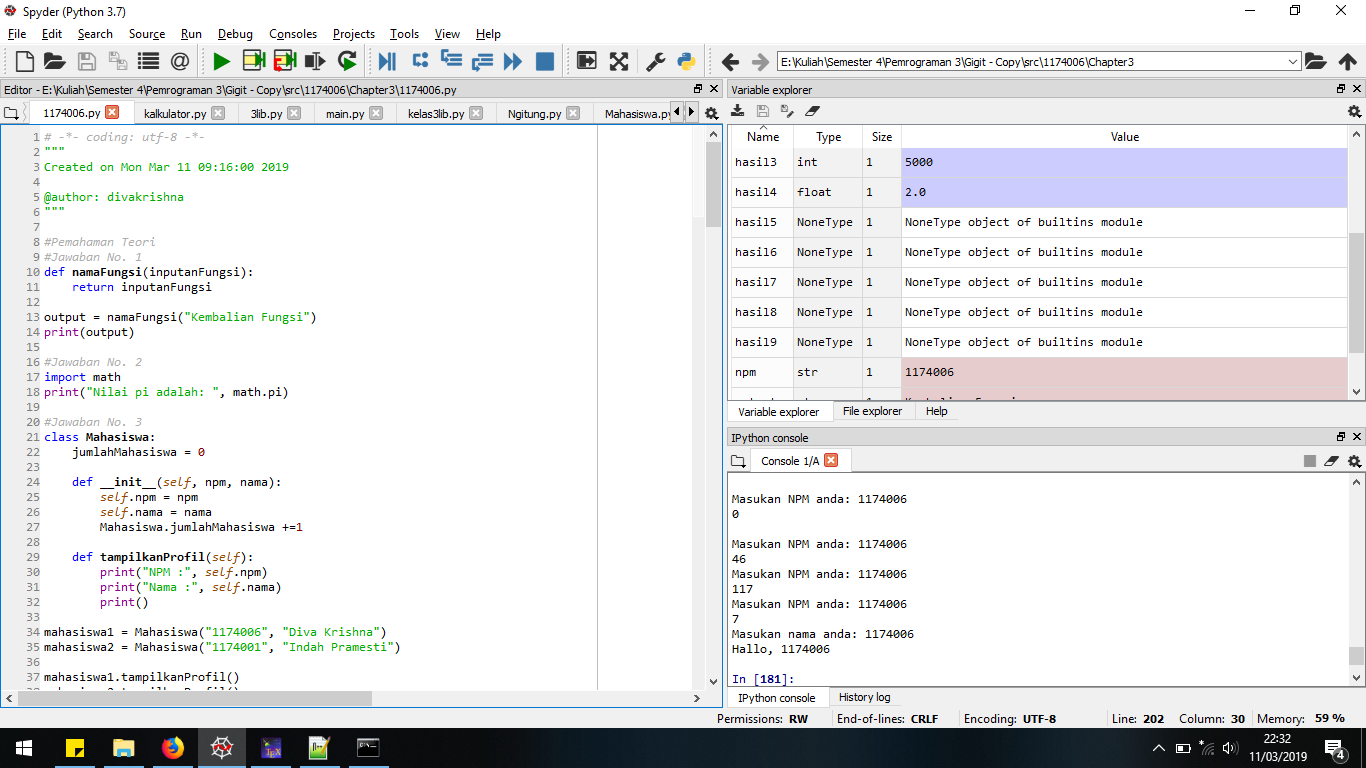
\includegraphics[width=10cm]{figures/diva/Chapter3/1174006_1.png}
	\centering
\end{figure}
\begin{figure}[H]
	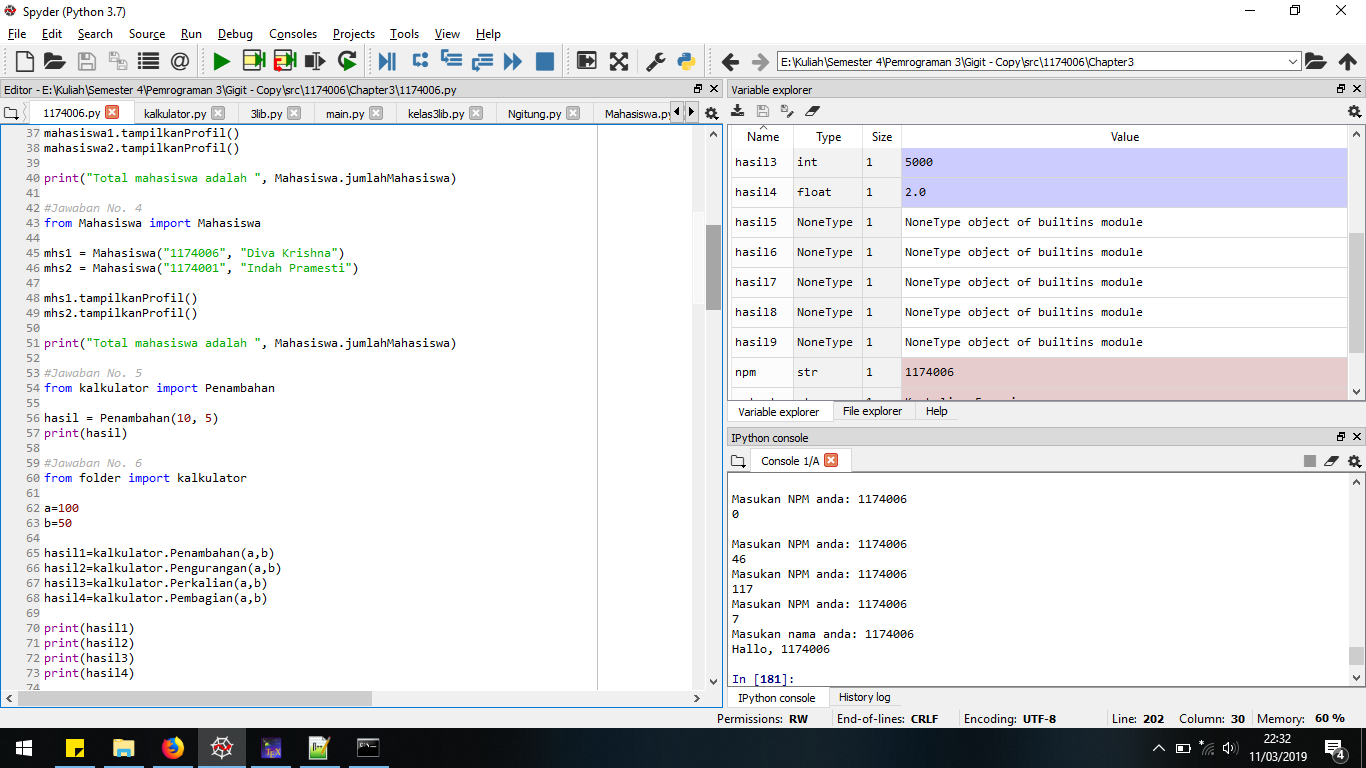
\includegraphics[width=10cm]{figures/diva/Chapter3/1174006_2.png}
	\centering
\end{figure}
\begin{figure}[H]
	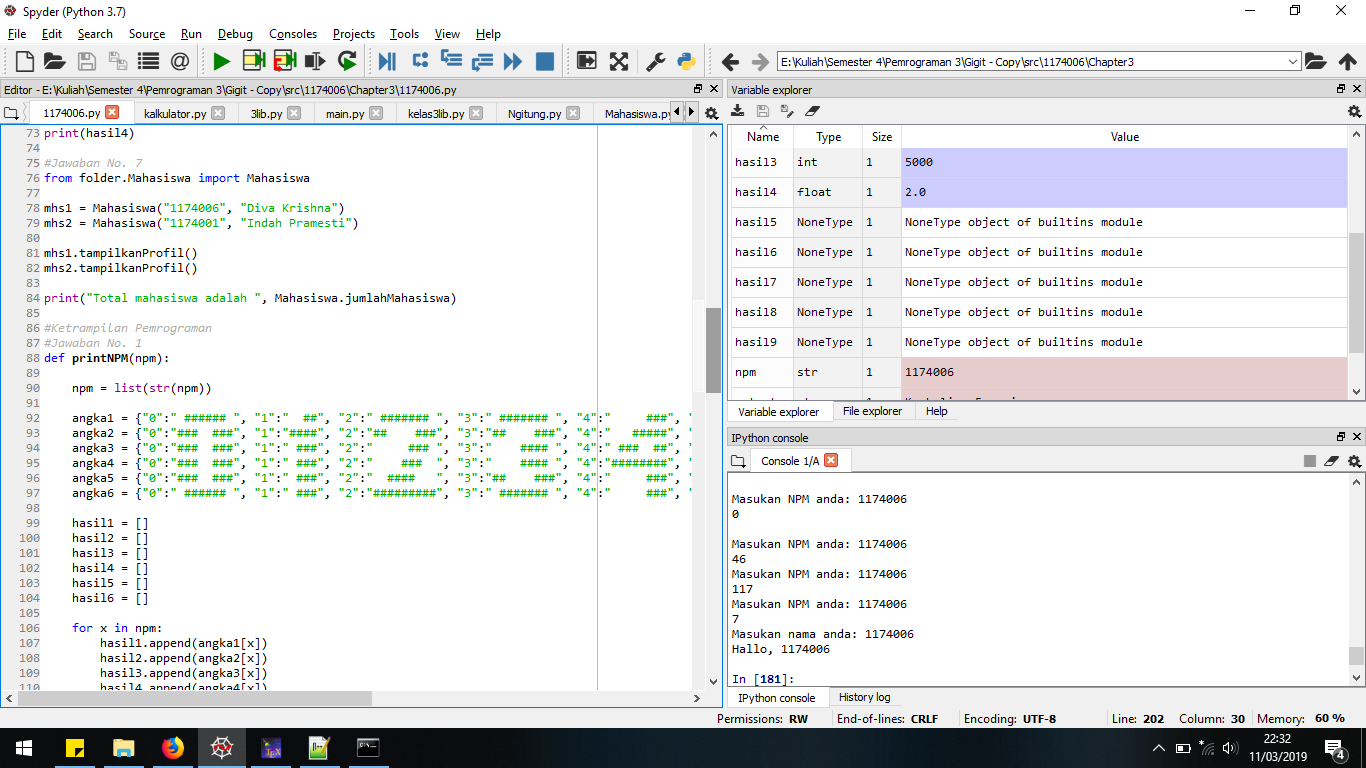
\includegraphics[width=10cm]{figures/diva/Chapter3/1174006_3.png}
	\centering
\end{figure}
\begin{figure}[H]
	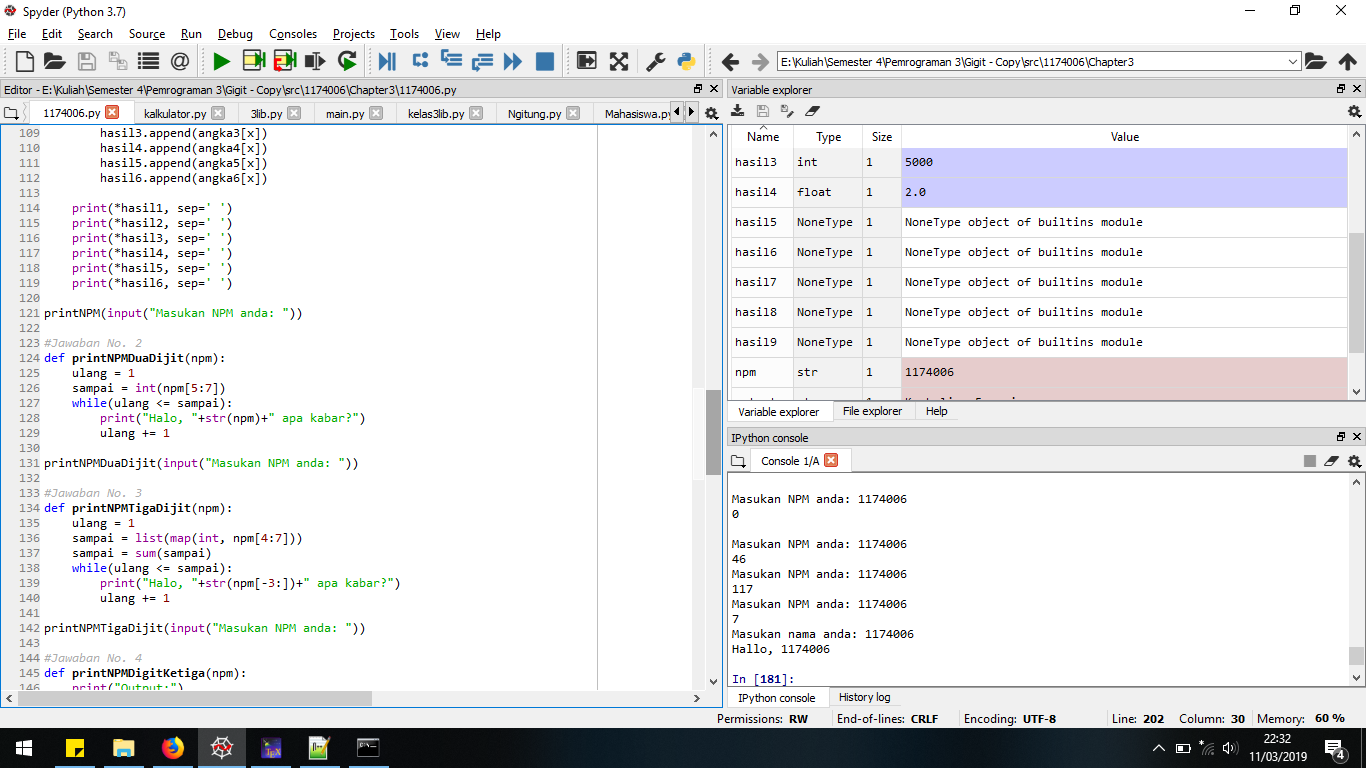
\includegraphics[width=10cm]{figures/diva/Chapter3/1174006_4.png}
	\centering
\end{figure}
\begin{figure}[H]
	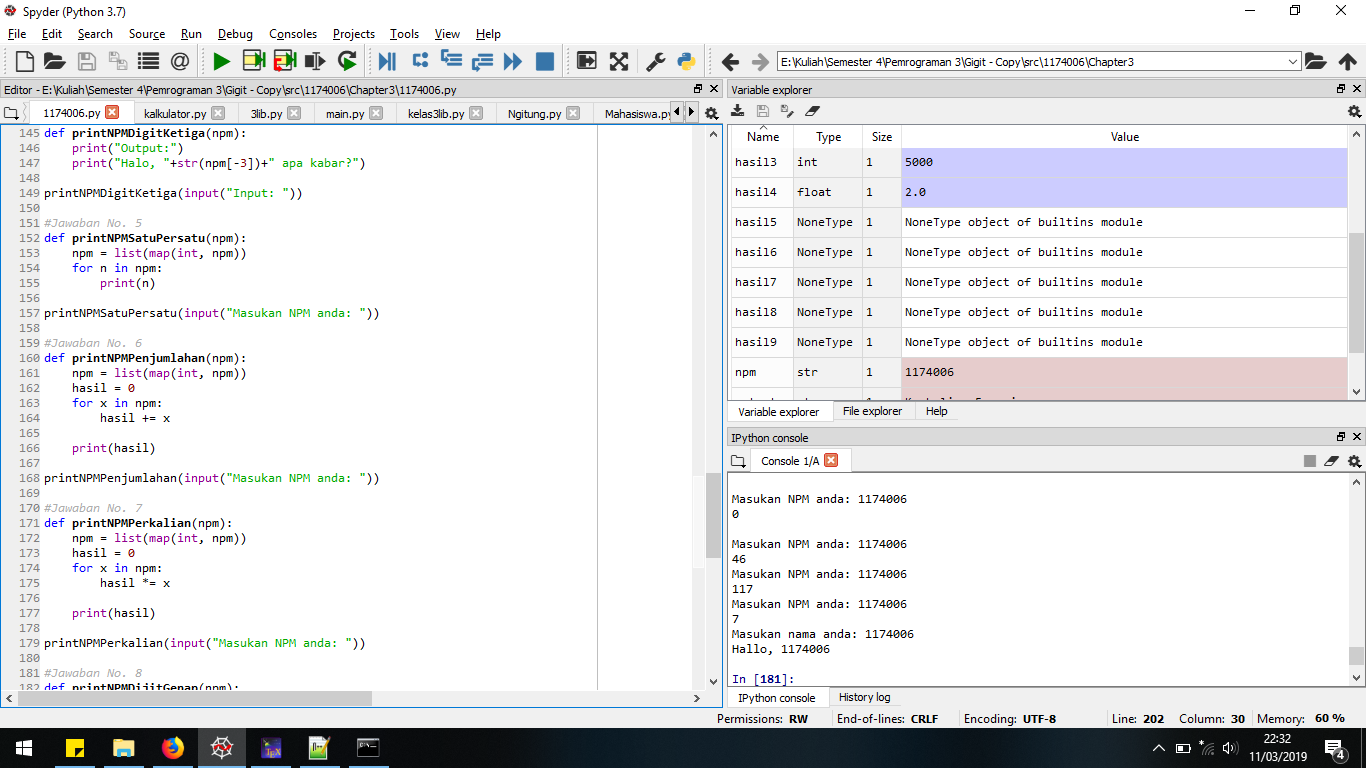
\includegraphics[width=10cm]{figures/diva/Chapter3/1174006_5.png}
	\centering
\end{figure}
\begin{figure}[H]
	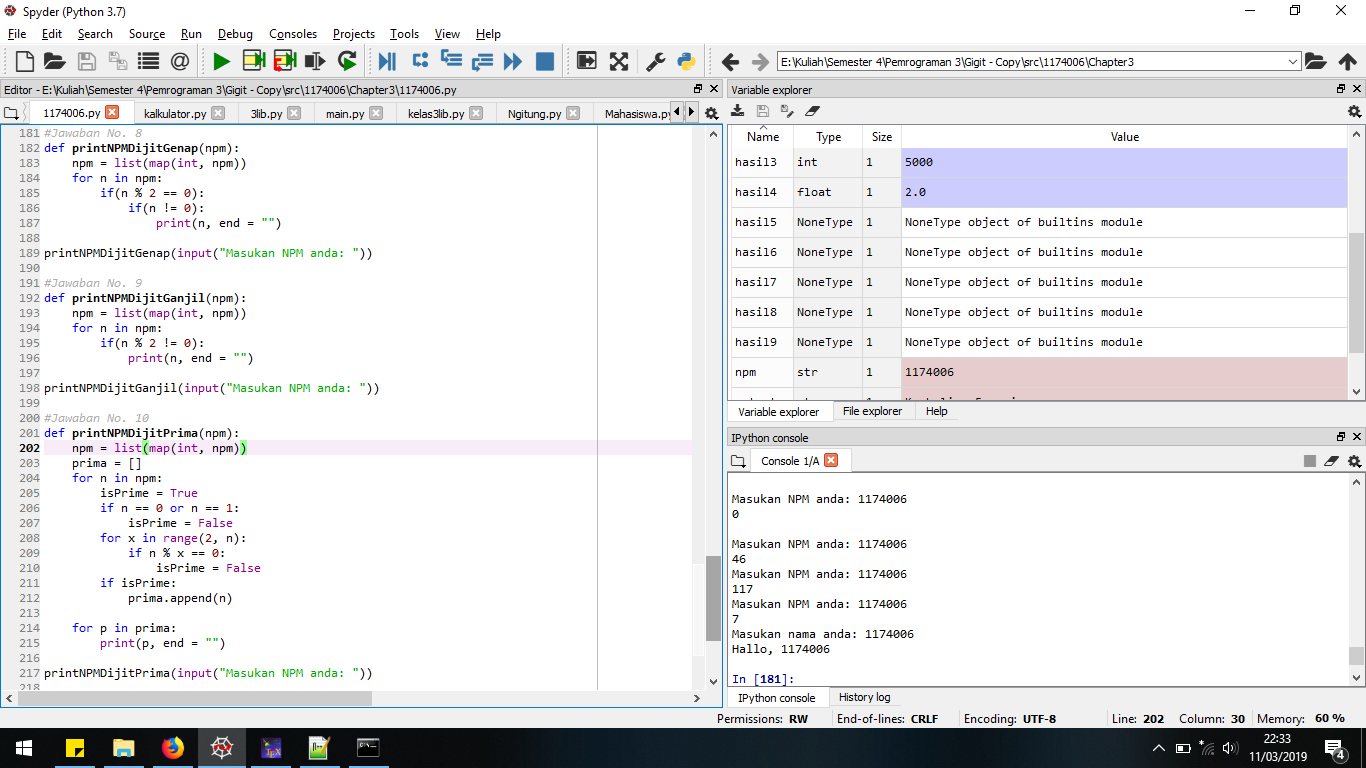
\includegraphics[width=10cm]{figures/diva/Chapter3/1174006_6.png}
	\centering
\end{figure}
\begin{figure}[H]
	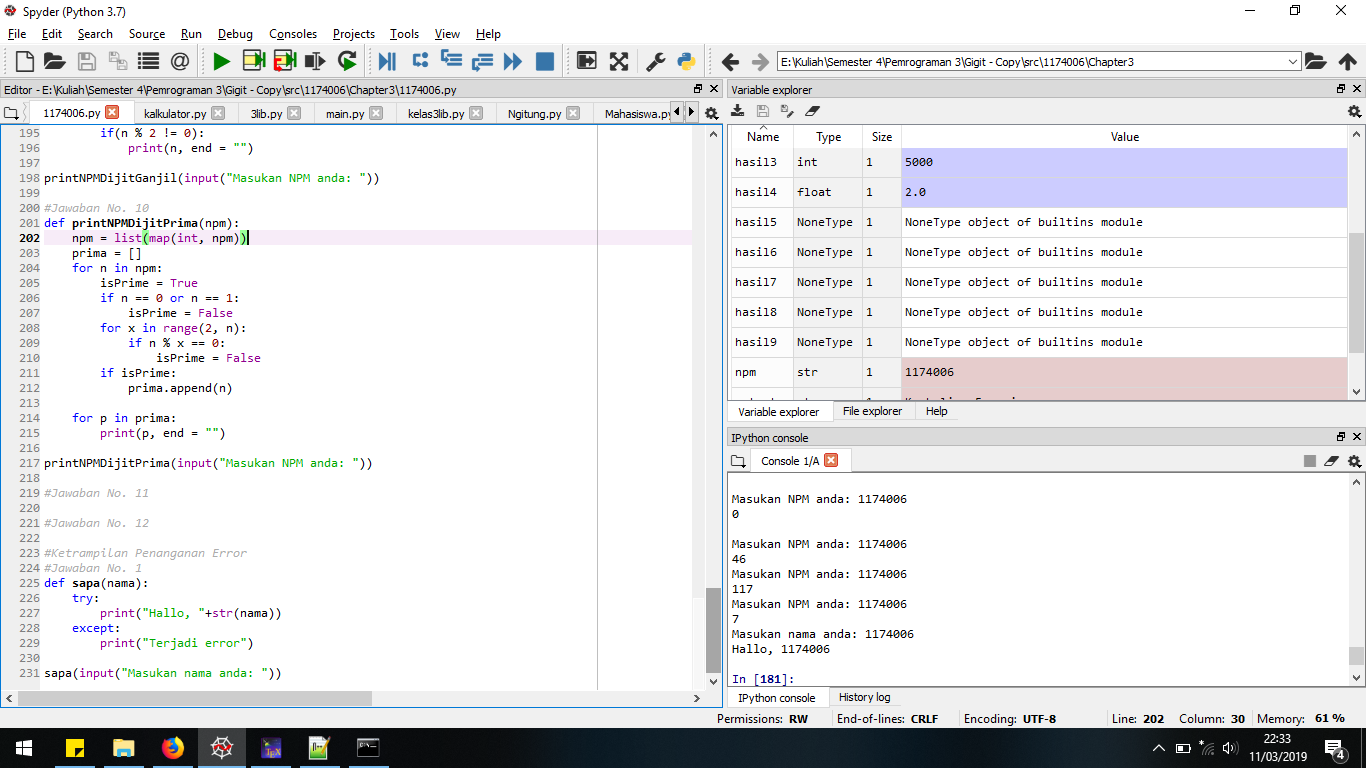
\includegraphics[width=10cm]{figures/diva/Chapter3/1174006_7.png}
	\centering
\end{figure}

\item Screenshoot Kodingan 3lib.py
\begin{figure}[H]
	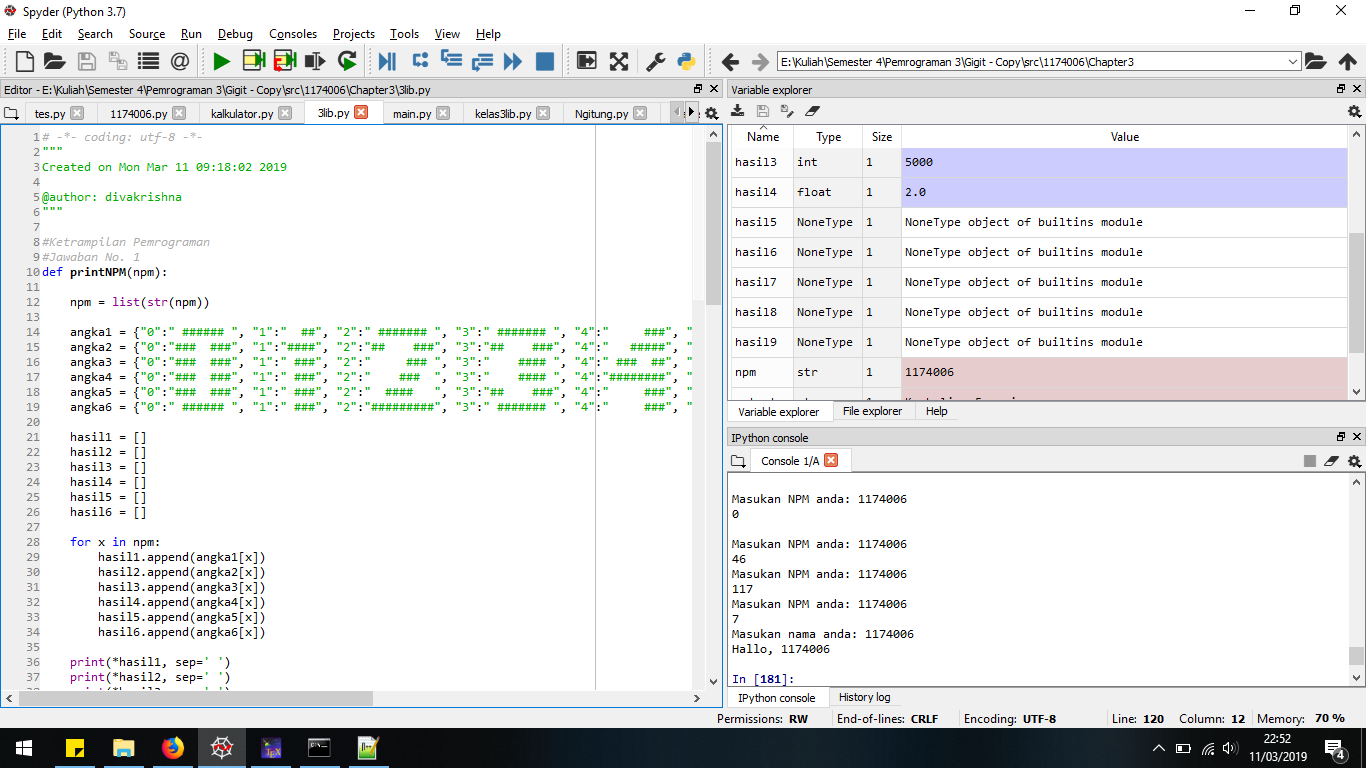
\includegraphics[width=10cm]{figures/diva/Chapter3/3lib_1.png}
	\centering
\end{figure}
\begin{figure}[H]
	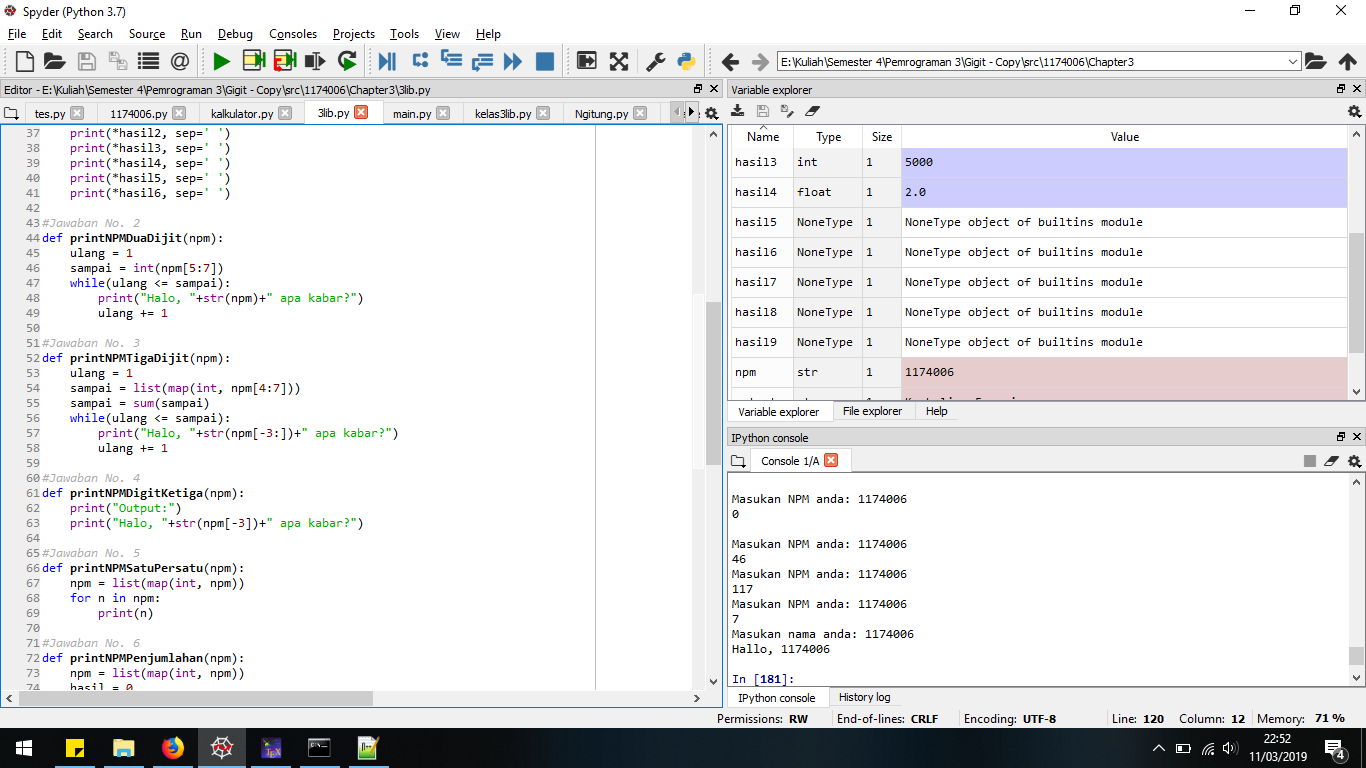
\includegraphics[width=10cm]{figures/diva/Chapter3/3lib_2.png}
	\centering
\end{figure}
\begin{figure}[H]
	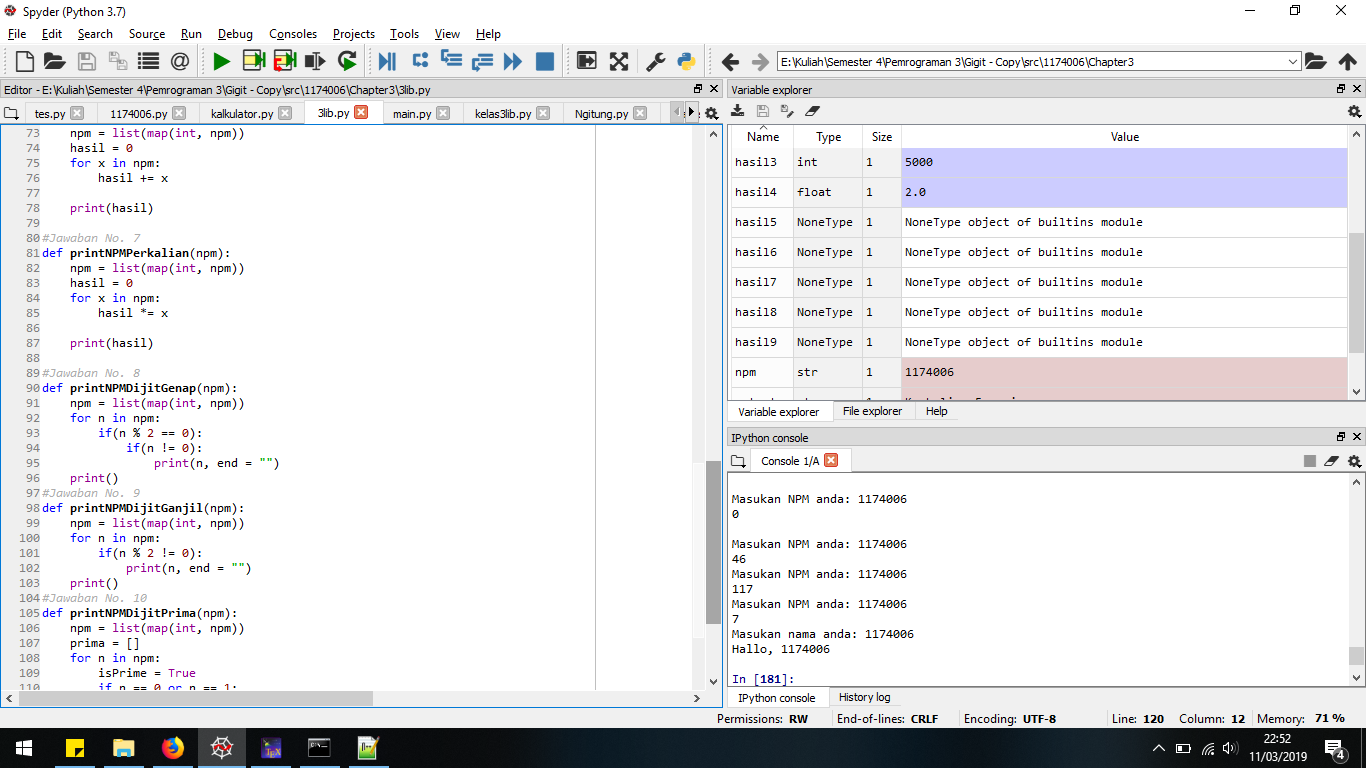
\includegraphics[width=10cm]{figures/diva/Chapter3/3lib_3.png}
	\centering
\end{figure}
\begin{figure}[H]
	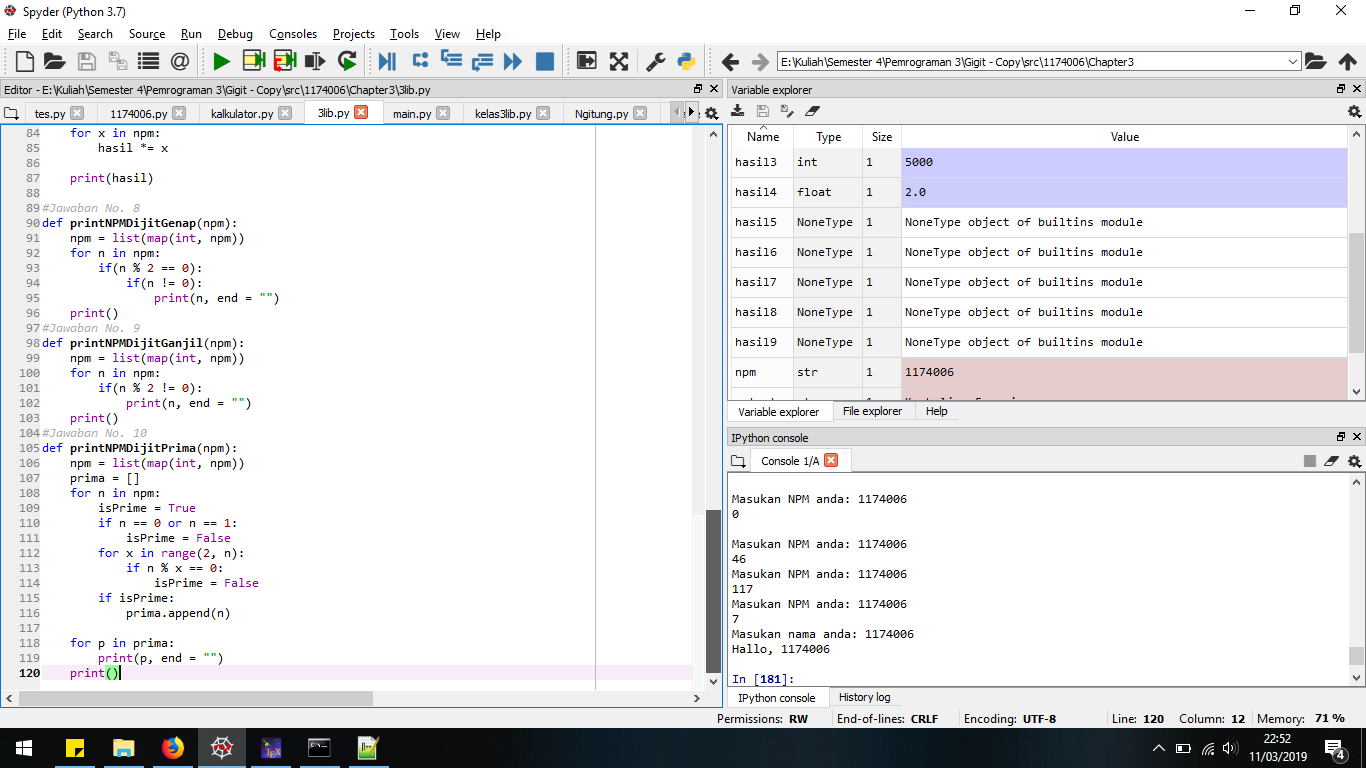
\includegraphics[width=10cm]{figures/diva/Chapter3/3lib_4.png}
	\centering
\end{figure}

\item Screenshoot Kodingan kelas3lib.py
\begin{figure}[H]
	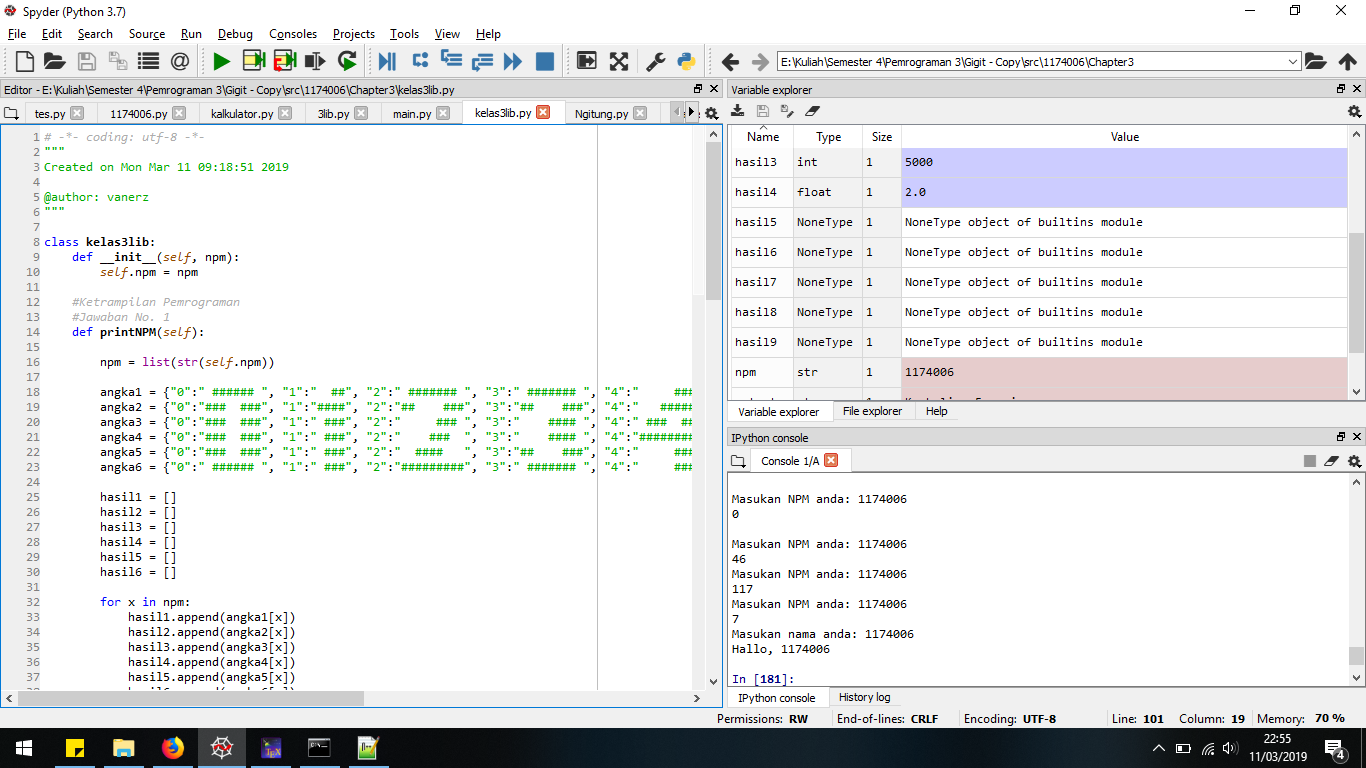
\includegraphics[width=10cm]{figures/diva/Chapter3/kelas3lib_1.png}
	\centering
\end{figure}
\begin{figure}[H]
	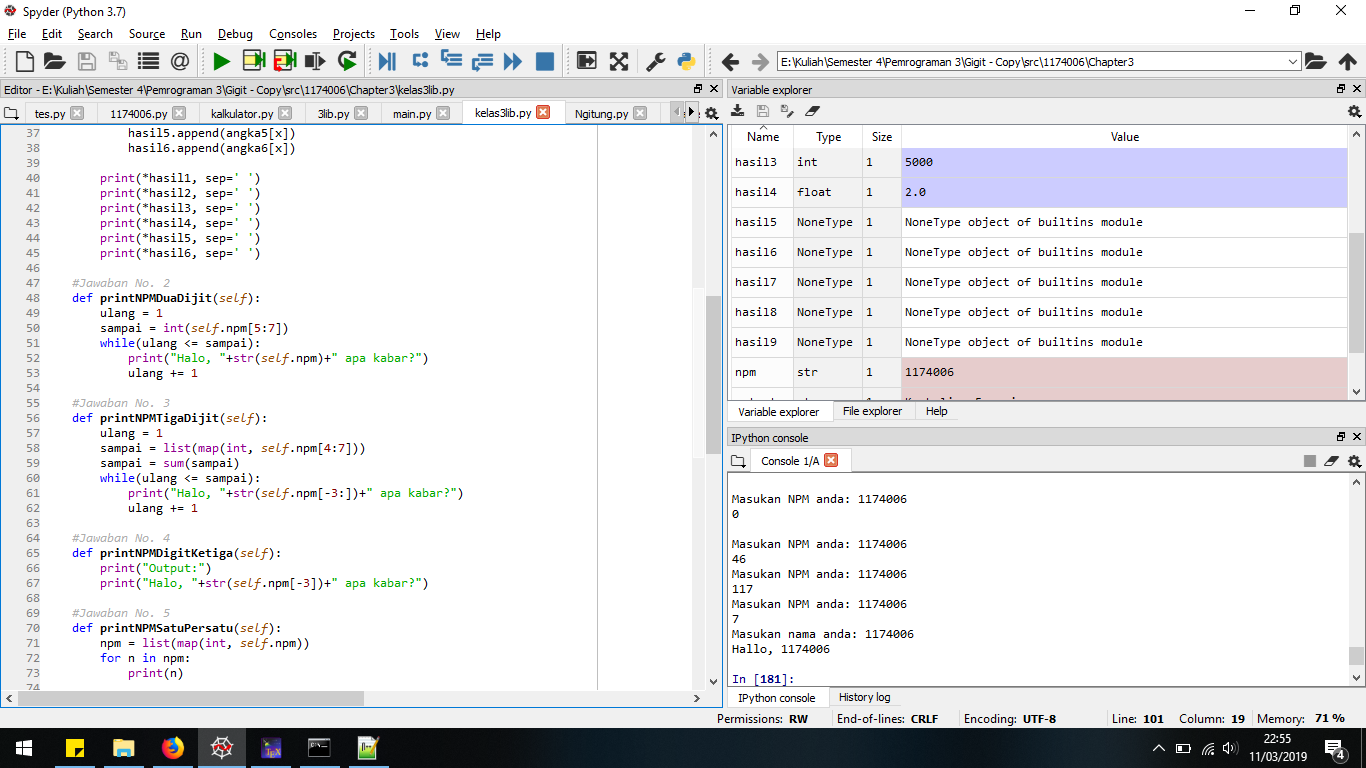
\includegraphics[width=10cm]{figures/diva/Chapter3/kelas3lib_2.png}
	\centering
\end{figure}
\begin{figure}[H]
	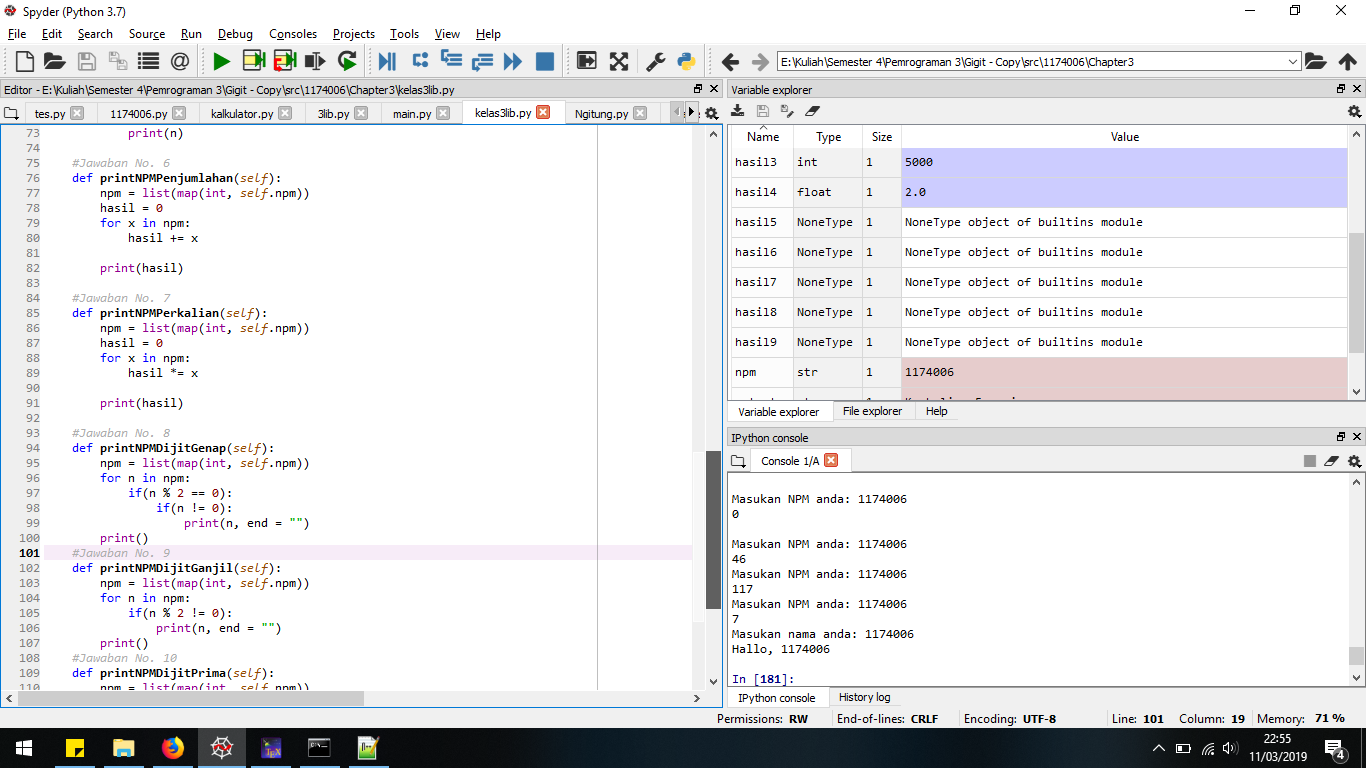
\includegraphics[width=10cm]{figures/diva/Chapter3/kelas3lib_3.png}
	\centering
\end{figure}
\begin{figure}[H]
	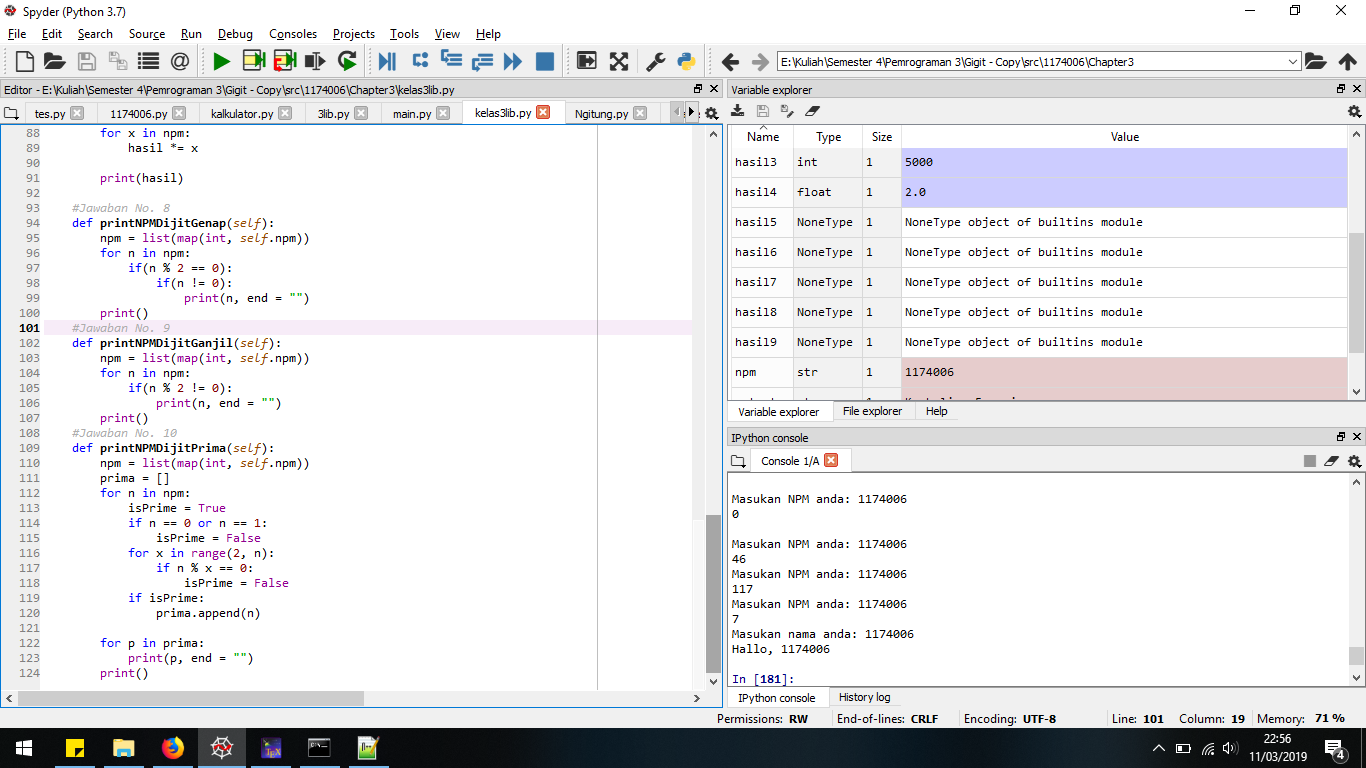
\includegraphics[width=10cm]{figures/diva/Chapter3/kelas3lib_4.png}
	\centering
\end{figure}

\item Screenshoot Kodingan main.py
\begin{figure}[H]
	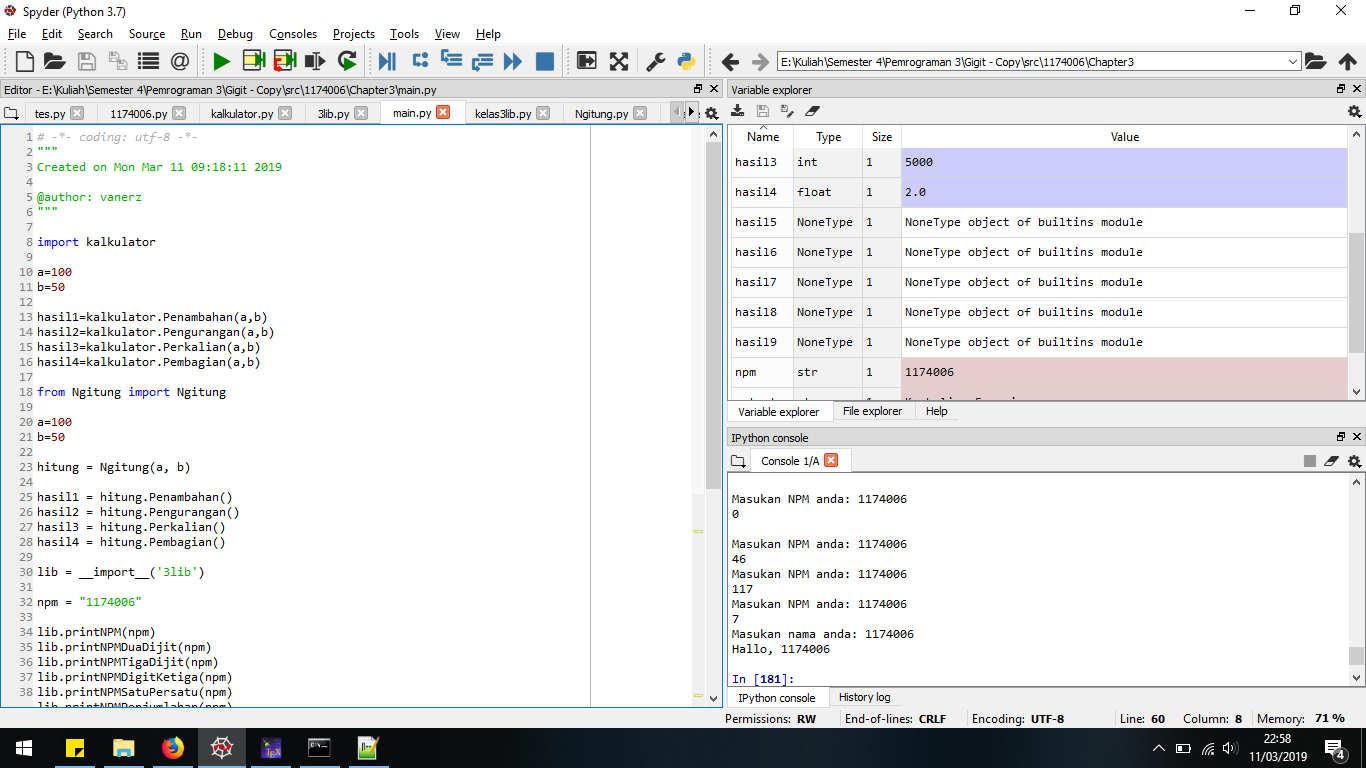
\includegraphics[width=10cm]{figures/diva/Chapter3/main_1.png}
	\centering
\end{figure}
\begin{figure}[H]
	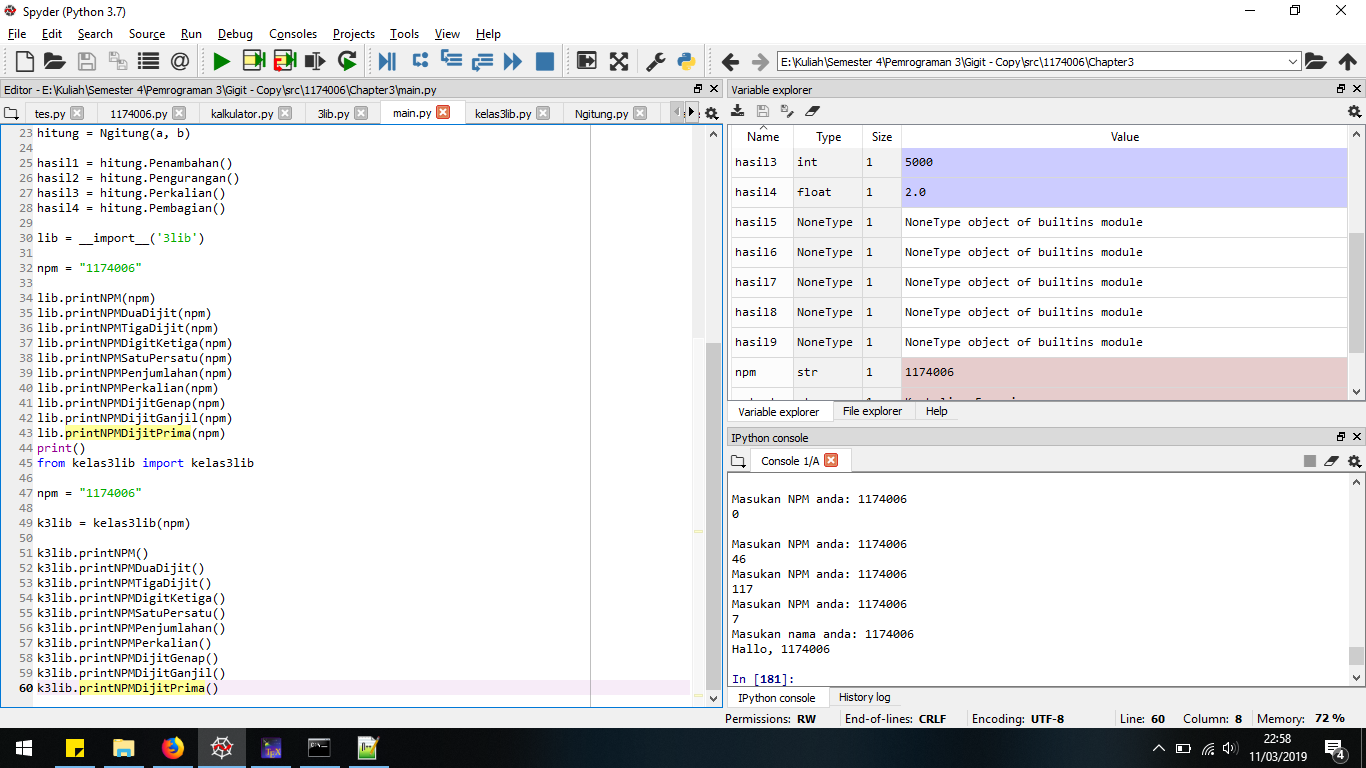
\includegraphics[width=10cm]{figures/diva/Chapter3/main_2.png}
	\centering
\end{figure}

\item Screenshoot Plagiarisme
\begin{figure}[H]
	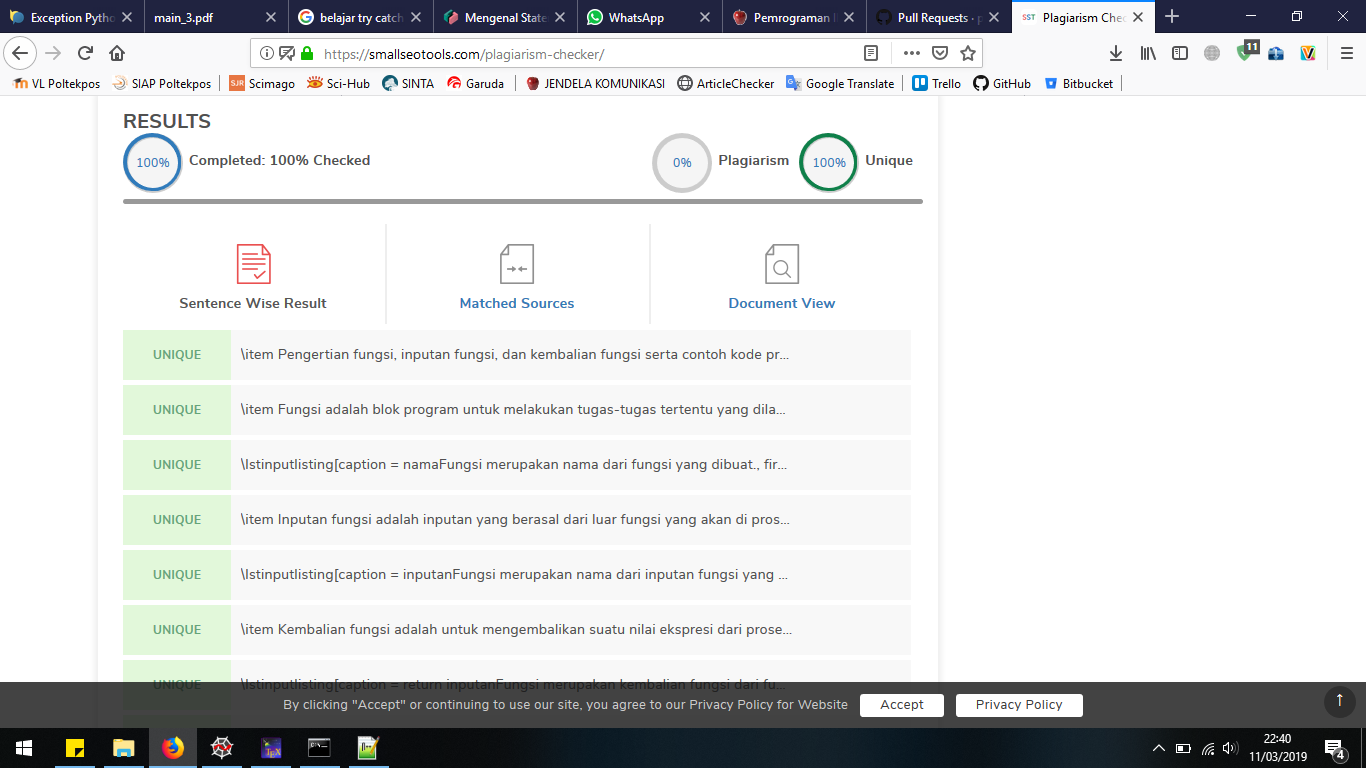
\includegraphics[width=10cm]{figures/diva/Chapter3/plagiarisme.png}
	\centering
\end{figure}
\end{enumerate}
%%%%%%%%%%%%%%%%%%%%%%%%%%%%%%%%%%%%%%%%%%%%%%%%%%%%%%%%%%%%%%
\section{Felix Setiawan Lase}
\subsubsection{Pemahanan Teori}
\begin{enumerate}
    \item Apa itu fungsi, inputan fungsi dan kembalian fungsi dengan contoh kode program
    lainnya.
    Fungsi adalah bagian dari program yang dapat digunakan ulang.
    Berikut merupakan contoh fungsi dan cara pemanggilannya
    \lstinputlisting[firstline=124, lastline=127]{src/1174026.py}

    Fungsi dapat membaca parameter, parameter adalah nilai yang disediakan kepada fungsi, dimana nilai ini akan menentukan output yang akan dihasilkan fungsi.
    \lstinputlisting[firstline=129, lastline=132]{src/1174026.py}

    Statemen return digunakan untuk keluar dari fungsi. Kita juga dapat menspesifikasikan nilai kembalian.
    \lstinputlisting[firstline=134, lastline=141]{src/1174026.py}

    \item Apa itu paket dan cara pemanggilan paket atau library dengan contoh kode
    program lainnya.
    Untuk memudahkan dalam pemanggilan fungsi yang di butuhkan, agar dapat dipanggil berulang.
    Cara pemanggilannya
    \lstinputlisting[firstline=143, lastline=144]{src/1174026.py}

    \item Jelaskan Apa itu kelas, apa itu objek, apa itu atribut, apa itu method dan
    contoh kode program lainnya masing-masing.
    kelas merupakan sebuah blueprint yang mepresentasikan objek.
    objek adalah hasil cetakan dadri sebuah kelas.
    method adalah suatu upaya yang digunakan oleh object.
    \lstinputlisting[firstline=146, lastline=168]{src/1174026.py}

    \item Jelaskan cara pemanggikan library kelas dari instansiasi dan pemakaiannya den-
    gan contoh program lainnya.
    Cara Pemanggilanya 
    \begin{itemize}
        \item pertama import terlebih dahulu filenya.
        \item kemudian buat variabel untuk menampung datanya
        \item setelah itu panggil nama classnya dan panggil methodnya
        \item Gunakan perintah print untuk menampilkan hasilnya

    \end{itemize}
    \lstinputlisting[firstline=170, lastline=175]{src/1174026.py}

    \item Jelaskan dengan contoh pemakaian paket dengan perintah from kalkulator im-
    port Penambahan disertai dengan contoh kode lainnya.
    Penggunaan paket from namafile import, itu berfungsi untuk memanggil file dan fungsinya
    \lstinputlisting[firstline=143, lastline=144]{src/1174026.py}

    \item Jelaskan dengan contoh kodenya, pemakaian paket fungsi apabila le library
    ada di dalam folder.
    Pemakaian paket adalah perkumpulan fungsi-fungsi. contoh kodenya adalah sebagai berikut :

    \item Jelaskan dengan contoh kodenya, pemakaian paket kelas apabila le library ada
    di dalam folder.
    \lstinputlisting[firstline=184, lastline=184]{src/1174026.py}

\end{enumerate}
\subsubsection{Ketrampilan Pemrograman}
\begin{enumerate}
    \item Buatlah fungsi dengan inputan variabel NPM, dan melakukan print luaran huruf
    yang dirangkai dari tanda bintang, pagar atau plus dari NPM kita. Tanda
    bintang untuk NPM mod 3=0, tanda pagar untuk NPM mod 3 =1, tanda plus
    untuk NPM mod3=2.
    \lstinputlisting[firstline=184, lastline=234]{src/1174026.py}

    \item Buatlah fungsi dengan inputan variabel berupa NPM. kemudian dengan meng-
    gunakan perulangan mengeluarkan print output sebanyak dua dijit belakang
    NPM.
    \lstinputlisting[firstline=237, lastline=243]{src/1174026.py}

    \item Buatlah fungsi dengan dengan input variabel string bernama NPM dan beri
    luaran output dengan perulangan berupa tiga karakter belakang dari NPM se-
    banyak penjumlahan tiga dijit tersebut.
    \lstinputlisting[firstline=245, lastline=255]{src/1174026.py}

    \item Buatlah fungsi hello word dengan input variabel string bernama NPM dan
    beri luaran output berupa digit ketiga dari belakang dari variabel NPM meng-
    gunakan akses langsung manipulasi string pada baris ketiga dari variabel NPM.
    \lstinputlisting[firstline=257, lastline=263]{src/1174026.py}

    \item buat fungsi program dengan input variabel NPM dan melakukan print nomor npm satu persatu kebawah.
    \lstinputlisting[firstline=265, lastline=269]{src/1174026.py}

    \item Buatlah fungsi dengan inputan variabel NPM, didalamnya melakukan penjum-
    lahan dari seluruh dijit NPM tersebut, wajib menggunakan perulangan dan
    atau kondisi.
    \lstinputlisting[firstline=272, lastline=279]{src/1174026.py}

    \item Buatlah fungsi dengan inputan variabel NPM, didalamnya melakukan melakukan
    perkalian dari seluruh dijit NPM tersebut, wajib menggunakan perulangan dan
    atau kondisi.
    \lstinputlisting[firstline=281, lastline=288]{src/1174026.py}

    \item Buatlah fungsi dengan inputan variabel NPM, Lakukan print NPM anda tapi
    hanya dijit genap saja. wajib menggunakan perulangan dan atau kondisi.
    \lstinputlisting[firstline=290, lastline=296]{src/1174026.py}

    \item Buatlah fungsi dengan inputan variabel NPM, Lakukan print NPM anda tapi
    hanya dijit ganjil saja. wajib menggunakan perulangan dan atau kondisi.
    \lstinputlisting[firstline=298, lastline=304]{src/1174026.py}

    \item Buatlah fungsi dengan inputan variabel NPM, Lakukan print NPM anda tapi
    hanya dijit yang termasuk bilangan prima saja. wajib menggunakan perulangan
    dan atau kondisi.
    \lstinputlisting[firstline=306, lastline=320]{src/1174026.py}

    \item Buatlah satu library yang berisi fungsi-fungsi dari nomor diatas dengan nama
    le 3lib.py dan berikan contoh cara pemanggilannya pada le main.py.
    \lstinputlisting[firstline=7, lastline=7]{src/main.py}

    \item Buatlah satu library class dengan nama le kelas3lib.py yang merupakan mod-
    ikasi dari fungsi-fungsi nomor diatas dan berikan contoh cara pemanggilannya
    pada le main.py.
    \lstinputlisting[firstline=8, lastline=9]{src/main.py}
    
\end{enumerate}
\subsubsection{Ketrampilan Penanganan Error}
Error yang di dapat dari mengerjakan tugas ini adalah type error, cara menaggulaginya dengan cara mengecheck kembali codingannya
kemudian run kembali aplikasinya
berikut contoh Penggunaan fungsi try dan exception
\lstinputlisting[firstline=177, lastline=182]{src/1174026.py}


%%%%%%%%%%%%%%%%%%%%%%%%%%%%%%%%%


\section{Dwi Septiani Tsaniyah}
\begin{enumerate}
    \item Apa itu fungsi, inputan fungsi dan kembalian fungsi dengan contoh kode program lainnya.
Fungsi memiliki tujuan agar kita dapat memecah program besar menjadi sub-sub program yang lebih sederhana. Pada saat kita membutuhkan suatu fitur maka kita tinggal memanggil fungsi yang telah kita buat. Fungsi pada python dibuat dengan kata kunci def dan diikuti dengan nama fungsi yang kita buat seperti contoh dibawah :
 \lstinputlisting[firstline=9, lastline=9]{src/1174003/1174003.py}

Inputan fungsi merupakan masukan yang kita berikan pada program dan program akan menampilkan hasil dari inputan yang kita masukkan. contoh dari inputan fungsi sebagai berikut :
 \lstinputlisting[firstline=12, lastline=14]{src/1174003/1174003.py}
Pengembalian fungsi memiliki tujuan untuk mengembalikan nilai dari hasil yang telah di proses. Dalam hal ini menggunakan kata kunci return yang diikuti dengan nilai atau variabel yang akan dikembalikan.
 \lstinputlisting[firstline=10, lastline=10]{src/1174003/1174003.py}

    \item Apa itu paket dan cara pemanggilan paket atau library dengan contoh kode program lainnya.
Library atau paket adalah modul-modul yang menyusun python. Modul-modul tersebut ditulis oleh berbagai orang dari seluruh dunia dan memiliki fungsi masing-masing untuk melakukan suatu hal. contoh kode programnya adalah sebagai berikut : from bte import penulisan print (penulisan(int(input(''Masukan NPM : ''))))
 \lstinputlisting[firstline=10, lastline=20]{src/1174003/1174003.py}

    \item Jelaskan Apa itu kelas, apa itu objek, apa itu atribut, apa itu method dan contoh kode program lainnya masing-masing.
kelas adalah Prototype yang ditentukan oleh pengguna untuk objek yang mendefinisikan seperangkat atribut yang menjadi ciri objek kelas apa pun. Objek ialah instansiasi atau perwujudan dari sebuah kelas. Bila kelas adalah prototipenya, dan objek adalah barang jadinya. Attribute adalah menggambarkan data yang dapat memberikan informasi kelas atau objek dimana attribut tersebut berada.
 \lstinputlisting[firstline=19, lastline=29]{src/1174003/1174003.py}

    \item Jelaskan cara pemanggilan library kelas dari instansiasi dan pemakaiannya dengan contoh program lainnya.
cara pemanggilan  library kelas dari instansiasi dan pemakaiannya adalah dengan cara meng-import library yang ada di dalam satu folder dan menggunakan kode berikut :
 \lstinputlisting[firstline=30, lastline=40]{src/1174003/1174003.py}

    \item Jelaskan dengan contoh pemakaian paket dengan perintah from kalkulator import Penambahan disertai dengan contoh kode lainnya.
contoh kodenya adalah sebagai berikut :
 \lstinputlisting[firstline=60, lastline=85]{src/1174003/1174003.py}

    \item Jelaskan dengan contoh kodenya, pemakaian paket fungsi apabila file library ada di dalam folder.
 Pemakaian paket adalah perkumpulan fungsi-fungsi. contoh kodenya adalah sebagai berikut :
 \lstinputlisting[firstline=90, lastline=100]{src/1174003/1174003.py}

    \item Jelaskan dengan contoh kodenya, pemakaian paket kelas apabila file library ada di dalam folder.
 \lstinputlisting[firstline=133, lastline=142]{src/1174003/1174003.py}
 \end{enumerate}

%%%%%%%%%%%%%%%%%%%%%%%%%%%%%%%%%%%%%%%%%%%%%%%%

\section{Dwi Yulianingsih}
\subsection{Pemahaman Teori}
\begin{enumerate}
    \item Apa itu fungsi, inputan fungsi dan kembalian fungsi dengan contoh kode program lainnya.
Fungsi memiliki tujuan agar kita dapat memecah program besar menjadi sub-sub program yang lebih sederhana. Pada saat kita membutuhkan suatu fitur maka kita tinggal memanggil fungsi yang telah kita buat. Fungsi pada python dibuat dengan kata kunci def dan diikuti dengan nama fungsi yang kita buat seperti contoh dibawah :
 \lstinputlisting[firstline=9, lastline=9]{src/1174009/tugas.py}
Inputan fungsi merupakan masukan yang kita berikan pada program dan program akan menampilkan hasil dari inputan yang kita masukkan. contoh dari inputan fungsi sebagai berikut :
 \lstinputlisting[firstline=12, lastline=14]{src/1174009/tugas.py}
Pengembalian fungsi memiliki tujuan untuk mengembalikan nilai dari hasil yang telah di proses. Dalam hal ini menggunakan kata kunci return yang diikuti dengan nilai atau variabel yang akan dikembalikan.
 \lstinputlisting[firstline=10, lastline=10]{src/1174009/tugas.py}

    \item Apa itu paket dan cara pemanggilan paket atau library dengan contoh kode program lainnya.
Library atau paket adalah modul-modul yang menyusun python. Modul-modul tersebut ditulis oleh berbagai orang dari seluruh dunia dan memiliki fungsi masing-masing untuk melakukan suatu hal. contoh kode programnya adalah sebagai berikut :
 \lstinputlisting[firstline=16, lastline=20]{src/1174009/tugas.py}

    \item Jelaskan Apa itu kelas, apa itu objek, apa itu atribut, apa itu method dan contoh kode program lainnya masing-masing.
kelas adalah Prototype yang ditentukan oleh pengguna untuk objek yang mendefinisikan seperangkat atribut yang menjadi ciri objek kelas apa pun. Objek ialah instansiasi atau perwujudan dari sebuah kelas. Bila kelas adalah prototipenya, dan objek adalah barang jadinya. Atribut adalah data anggota (variabel kelas dan variabel contoh) dan metode, diakses melalui notasi titik. Sedangkan method fungsi yang didefinisikan di dalam suatu kelas.
 \lstinputlisting[firstline=23, lastline=32]{src/1174009/tugas.py}

    \item Jelaskan cara pemanggilan library kelas dari instansiasi dan pemakaiannya dengan contoh program lainnya.
cara pemanggilan  library kelas dari instansiasi dan pemakaiannya adalah dengan cara meng-import library yang ada di dalam satu folder dan menggunakan kode berikut :
 \lstinputlisting[firstline=34, lastline=40]{src/1174009/tugas.py}

    \item Jelaskan dengan contoh pemakaian paket dengan perintah from kalkulator import Penambahan disertai dengan contoh kode lainnya.
Penggunaan paket berfungsi untuk memanggil file dan fungsinya. contoh kodenya adalah sebagai berikut :
 \lstinputlisting[firstline=42, lastline=44]{src/1174009/tugas.py}

    \item Jelaskan dengan contoh kodenya, pemakaian paket fungsi apabila file library ada di dalam folder.
 Pemakaian paket adalah perkumpulan fungsi-fungsi. contoh kodenya adalah sebagai berikut :
 \lstinputlisting[firstline=46, lastline=55]{src/1174009/tugas.py}

    \item Jelaskan dengan contoh kodenya, pemakaian paket kelas apabila file library ada di dalam folder.
 \lstinputlisting[firstline=62, lastline=67]{src/1174009/tugas.py}

\end{enumerate}

\subsection{Praktek}
\begin{enumerate}
    \item jawaban no 1
 \lstinputlisting[firstline=8, lastline=43]{src/1174009/1174009.py}

    \item jawaban no 2
 \lstinputlisting[firstline=45, lastline=51]{src/1174009/1174009.py}

    \item jawaban no 3
 \lstinputlisting[firstline=53, lastline=61]{src/1174009/1174009.py}

    \item jawaban no 4
 \lstinputlisting[firstline=63, lastline=68]{src/1174009/1174009.py}

    \item jawaban no 5
 \lstinputlisting[firstline=70, lastline=75]{src/1174009/1174009.py}

    \item jawaban no 6
 \lstinputlisting[firstline=77, lastline=83]{src/1174009/1174009.py}

    \item jawaban no 7
 \lstinputlisting[firstline=85, lastline=91]{src/1174009/1174009.py}

    \item jawaban no 8
 \lstinputlisting[firstline=93, lastline=100]{src/1174009/1174009.py}

    \item jawaban no 9
 \lstinputlisting[firstline=103, lastline=108]{src/1174009/1174009.py}

    \item jawaban no 10
 \lstinputlisting[firstline=110, lastline=126]{src/1174009/1174009.py}

    \item jawaban 11
 \lstinputlisting[firstline=8, lastline=21]{src/1174009/main.py}

    \item jawaban 12
 \lstinputlisting[firstline=23, lastline=38]{src/1174009/main.py}
\end{enumerate}

\subsection{Penanganan Eror}
untuk menangani eror yang terjadi bisa menggunakan source kode dibawah ini :
 \lstinputlisting[firstline=69, lastline=75]{src/1174009/tugas.py}

\begin{figure}[!Htbp]
\centering
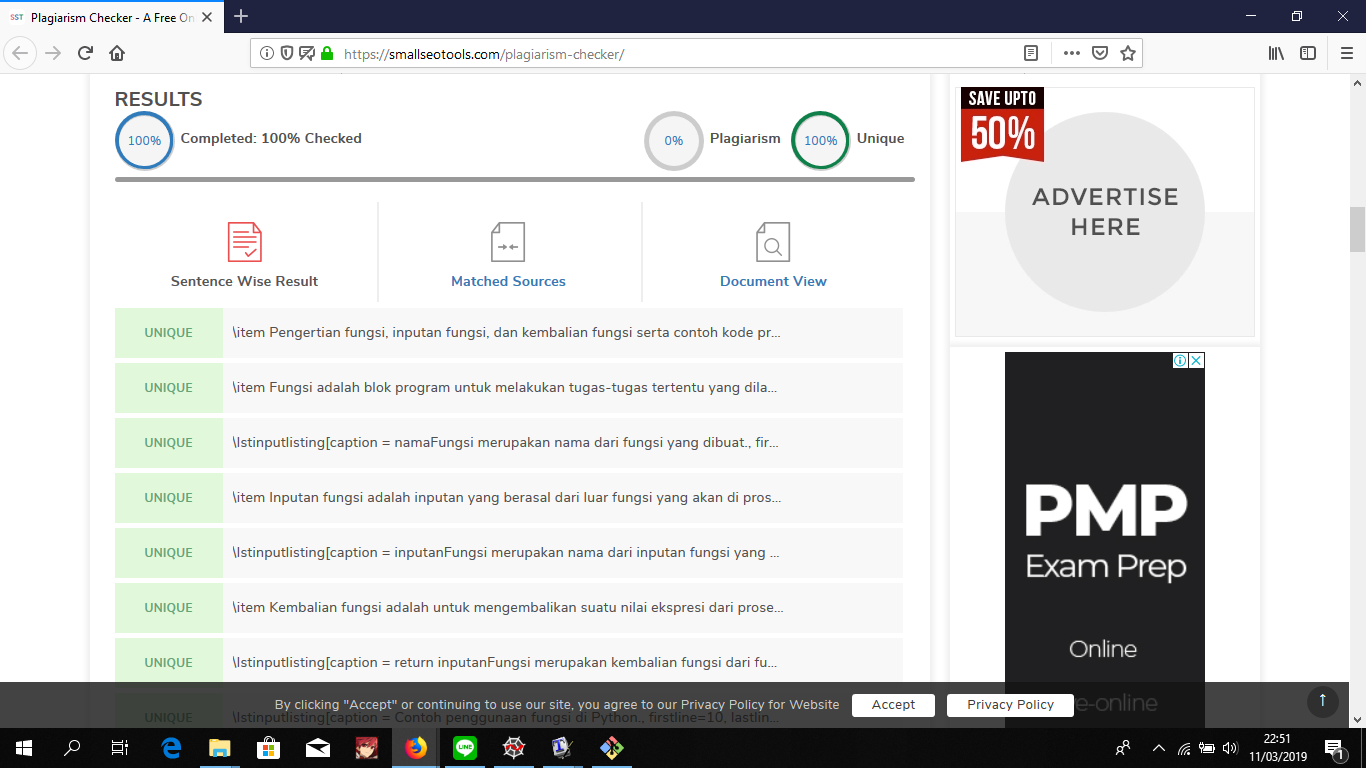
\includegraphics[width=6cm,height=6cm]{figures/Wiyul.png}
\caption{SS Bebas Plagiarisme}
\label{dwiyul}
\end{figure}
%%%%%%%%%%%%%%%%%%%%%%%%%%%%%%%%%%%%%%%%%%%%%%%%%%%%%%%%%%%%%%%%%%%%%%%%%%%%%%%%%%%%%%%%%%%%%%%%%%%%%%%%%%%%%%%%


\section{Choirul Anam}
\subsubsection{Pemahaman Teori}
\begin{enumerate}
    \item Apa itu fungsi, inputan fungsi dan kembalian fungsi dengan contoh kode program
    lainnya.
    Fungsi adalah suatu perintah diaman perintah tersebut dapat di panggil berulang ulang.
    Berikut merupakan contoh fungsi dan cara pemanggilannya
    \lstinputlisting[firstline=184, lastline=187]{src/1174004.py}

    Fungsi juga bisa membaca parameter, dimana parameter adalah nilai yang di inputkan atau di lemparkan untuk kebutuhan fungsi, dimana nilai ini akan menentukan output yang akan dihasilkan fungsi.
    \lstinputlisting[firstline=189, lastline=192]{src/1174004.py}

    Statemen return digunakan untuk keluar dari fungsi. Kita juga dapat menspesifikasikan nilai kembalian.
    \lstinputlisting[firstline=194, lastline=201]{src/1174004.py}

    \item Apa itu paket dan cara pemanggilan paket atau library dengan contoh kode
    program lainnya.
    Untuk memudahkan dalam pemanggilan fungsi yang di butuhkan, agar dapat dipanggil berulang.
    Cara pemanggilannya
    \lstinputlisting[firstline=203, lastline=204]{src/1174004.py}

    \item Jelaskan Apa itu kelas, apa itu objek, apa itu atribut, apa itu method dan
    contoh kode program lainnya masing-masing.
    kelas merupakan sebuah blueprint yang mepresentasikan objek.
    objek adalah hasil cetakan dadri sebuah kelas.
    method adalah suatu upaya yang digunakan oleh object.
    atribut adalah apasaja yang dapat dilakukan oleh objek
    \lstinputlisting[firstline=206, lastline=228]{src/1174004.py}

    \item Jelaskan cara pemanggilan library kelas dari instansiasi dan pemakaiannya den-
    gan contoh program lainnya.
    Cara Pemanggilanya 
    \begin{itemize}
        \item import file.
        \item kemudian buat variabel untuk menampung datanya
        \item setelah itu panggil nama classnya dan panggil methodnya
        \item Gunakan perintah print untuk menampilkan hasilnya

    \end{itemize}
    \lstinputlisting[firstline=230, lastline=235]{src/1174004.py}

    \item Jelaskan dengan contoh pemakaian paket dengan perintah from kalkulator im-
    port Penambahan disertai dengan contoh kode lainnya.
    Penggunaan paket from namafile import, itu berfungsi untuk memanggil file dan fungsinya
    \lstinputlisting[firstline=203, lastline=204]{src/1174004.py}

    \item Jelaskan dengan contoh kodenya, pemakaian paket fungsi apabila le library
    ada di dalam folder.
    Pemakaian paket adalah perkumpulan fungsi-fungsi. contoh kodenya adalah sebagai berikut :

    \item Jelaskan dengan contoh kodenya, pemakaian paket kelas apabila le library ada
    di dalam folder.
    \lstinputlisting[firstline=244, lastline=244]{src/1174004.py}

\end{enumerate}
\subsubsection{Ketrampilan Pemrograman}
\begin{enumerate}
    \item Buatlah fungsi dengan inputan variabel NPM, dan melakukan print luaran huruf
    yang dirangkai dari tanda bintang, pagar atau plus dari NPM kita. Tanda
    bintang untuk NPM mod 3=0, tanda pagar untuk NPM mod 3 =1, tanda plus
    untuk NPM mod3=2.
    \lstinputlisting[firstline=245, lastline=294]{src/1174004.py}

    \item Buatlah fungsi dengan inputan variabel berupa NPM. kemudian dengan meng-
    gunakan perulangan mengeluarkan print output sebanyak dua dijit belakang
    NPM.
    \lstinputlisting[firstline=297, lastline=303]{src/1174004.py}

    \item Buatlah fungsi dengan dengan input variabel string bernama NPM dan beri
    luaran output dengan perulangan berupa tiga karakter belakang dari NPM se-
    banyak penjumlahan tiga dijit tersebut.
    \lstinputlisting[firstline=306, lastline=315]{src/1174004.py}

    \item Buatlah fungsi hello word dengan input variabel string bernama NPM dan
    beri luaran output berupa digit ketiga dari belakang dari variabel NPM meng-
    gunakan akses langsung manipulasi string pada baris ketiga dari variabel NPM.
    \lstinputlisting[firstline=318, lastline=323]{src/1174004.py}

    \item buat fungsi program dengan input variabel NPM dan melakukan print nomor npm satu persatu kebawah.
    \lstinputlisting[firstline=326, lastline=330]{src/1174004.py}

    \item Buatlah fungsi dengan inputan variabel NPM, didalamnya melakukan penjum-
    lahan dari seluruh dijit NPM tersebut, wajib menggunakan perulangan dan
    atau kondisi.
    \lstinputlisting[firstline=333, lastline=339]{src/1174004.py}

    \item Buatlah fungsi dengan inputan variabel NPM, didalamnya melakukan melakukan
    perkalian dari seluruh dijit NPM tersebut, wajib menggunakan perulangan dan
    atau kondisi.
    \lstinputlisting[firstline=342, lastline=348]{src/1174004.py}

    \item Buatlah fungsi dengan inputan variabel NPM, Lakukan print NPM anda tapi
    hanya dijit genap saja. wajib menggunakan perulangan dan atau kondisi.
    \lstinputlisting[firstline=351, lastline=356]{src/1174004.py}

    \item Buatlah fungsi dengan inputan variabel NPM, Lakukan print NPM anda tapi
    hanya dijit ganjil saja. wajib menggunakan perulangan dan atau kondisi.
    \lstinputlisting[firstline=359, lastline=364]{src/1174004.py}

    \item Buatlah fungsi dengan inputan variabel NPM, Lakukan print NPM anda tapi
    hanya dijit yang termasuk bilangan prima saja. wajib menggunakan perulangan
    dan atau kondisi.
    \lstinputlisting[firstline=367, lastline=380]{src/1174004.py}

    \item Buatlah satu library yang berisi fungsi-fungsi dari nomor diatas dengan nama
    le 3lib.py dan berikan contoh cara pemanggilannya pada le main.py.
    \lstinputlisting[firstline=7, lastline=7]{src/main.py}

    \item Buatlah satu library class dengan nama le kelas3lib.py yang merupakan mod-
    ikasi dari fungsi-fungsi nomor diatas dan berikan contoh cara pemanggilannya
    pada le main.py.
    \lstinputlisting[firstline=8, lastline=9]{src/main.py}
    
\end{enumerate}
\subsubsection{Ketrampilan Penanganan Error}
Error yang di dapat dari mengerjakan tugas ini adalah type error, cara menaggulaginya dengan cara mengecheck kembali codingannya
kemudian run kembali aplikasinya
berikut contoh Penggunaan fungsi try dan exception
\lstinputlisting[firstline=177, lastline=182]{src/1174004.py}

%%%%%%%%%%%%%%%%%%%%%%%%%%%%%%%%%%%%%%%%%%%%%%%%%%%%%%%%%%%%%%
\section{Muh. Rifky Prananda}
\subsubsection{Pemahanan Teori}
\begin{enumerate}
    \item Apa itu fungsi, inputan fungsi dan kembalian fungsi dengan contoh kode program
    lainnya.
    Fungsi adalah salah satu bagian dari program yang dapat digunakan ulang.
    Berikut merupakan contoh fungsi dan cara pemanggilannya
    \lstinputlisting[firstline=74, lastline=77]{src/1174017.py}

    Fungsi bisa membaca parameter, parameter yaitu sebuah nilai yang tersedia untuk fungsi, dimana pada nilai ini menentukan output yang dihasilkan fungsi.
    \lstinputlisting[firstline=79, lastline=82]{src/1174017.py}

    Statemen return dapat digunakan untuk bisa keluar dari fungsi. Kita juga dapat menspesifikasikan nilai kembalian.
    \lstinputlisting[firstline=84, lastline=91]{src/1174017.py}

    \item Apa itu paket dan cara pemanggilan paket atau library dengan contoh kode
    program lainnya.
    Untuk bisa lebih memudahkan dalam pemanggilan fungsi yang dibutuhkan, agar dapat dipanggil berulang-ulang.
    Cara pemanggilannya
    \lstinputlisting[firstline=93, lastline=94]{src/1174017.py}

    \item Jelaskan Apa itu kelas, apa itu objek, apa itu atribut, apa itu method dan
    contoh kode program lainnya masing-masing.
    kelas adalah sebuah blueprint yang mempresentasikan suatu objek.
    objek yaitu hasil cetakan dari sebuah kelas itu sendiri.
    method adalah sifat atau perilaku dari object.
    \lstinputlisting[firstline=96, lastline=98]{src/1174017.py}

    \item Jelaskan cara pemanggikan library kelas dari instansiasi dan pemakaiannya den-
    gan contoh program lainnya.
    Cara Pemanggilanya 
    \begin{itemize}
        \item yang pertama import terlebih dahulu filenya.
        \item selanjutnya buat variabel untuk dapat menampung datanya
        \item kemudian panggil nama classnya dan panggil methodnya
        \item Gunakan suatu perintah print untuk menampilkan hasilnya

    \end{itemize}
    \lstinputlisting[firstline=120, lastline=125]{src/1174017.py}

    \item Jelaskan dengan contoh pemakaian paket dengan perintah from kalkulator im-
    port Penambahan disertai dengan contoh kode lainnya.
    Penggunaan paket from namafile import itu berfungsi untuk dapat memanggil file dan fungsinya
    \lstinputlisting[firstline=143, lastline=144]{src/1174017.py}

    \item Jelaskan dengan contoh kodenya, pemakaian paket fungsi apabila le library
    ada di dalam folder.
    Pemakaian paket adalah suatu perkumpulan fungsi-fungsi. contoh kodenya adalah sebagai berikut :

    \item Jelaskan dengan contoh kodenya, pemakaian paket kelas apabila le library ada
    di dalam folder.
    \lstinputlisting[firstline=184, lastline=184]{src/1174017.py}

\end{enumerate}
\subsubsection{Ketrampilan Pemrograman}
\begin{enumerate}
    \item Buatlah fungsi dengan inputan variabel NPM, dan melakukan print luaran huruf
    yang dirangkai dari tanda bintang, pagar atau plus dari NPM kita. Tanda
    bintang untuk NPM mod 3=0, tanda pagar untuk NPM mod 3 =1, tanda plus
    untuk NPM mod3=2.
    \lstinputlisting[firstline=143, lastline=190]{src/1174017.py}

    \item Buatlah fungsi dengan inputan variabel berupa NPM. kemudian dengan meng-
    gunakan perulangan mengeluarkan print output sebanyak dua dijit belakang
    NPM.
    \lstinputlisting[firstline=192, lastline=197]{src/1174017.py}

    \item Buatlah fungsi dengan dengan input variabel string bernama NPM dan beri
    luaran output dengan perulangan berupa tiga karakter belakang dari NPM se-
    banyak penjumlahan tiga dijit tersebut.
    \lstinputlisting[firstline=199, lastline=207]{src/1174017.py}

    \item Buatlah fungsi hello word dengan input variabel string bernama NPM dan
    beri luaran output berupa digit ketiga dari belakang dari variabel NPM meng-
    gunakan akses langsung manipulasi string pada baris ketiga dari variabel NPM.
    \lstinputlisting[firstline=209, lastline=213]{src/1174017.py}

    \item buat fungsi program dengan input variabel NPM dan melakukan print nomor npm satu persatu kebawah.
    \lstinputlisting[firstline=215, lastline=218]{src/1174017.py}

    \item Buatlah fungsi dengan inputan variabel NPM, didalamnya melakukan penjum-
    lahan dari seluruh dijit NPM tersebut, wajib menggunakan perulangan dan
    atau kondisi.
    \lstinputlisting[firstline=220, lastline=225]{src/1174017.py}

    \item Buatlah fungsi dengan inputan variabel NPM, didalamnya melakukan melakukan
    perkalian dari seluruh dijit NPM tersebut, wajib menggunakan perulangan dan
    atau kondisi.
    \lstinputlisting[firstline=227, lastline=232]{src/1174017.py}

    \item Buatlah fungsi dengan inputan variabel NPM, Lakukan print NPM anda tapi
    hanya dijit genap saja. wajib menggunakan perulangan dan atau kondisi.
    \lstinputlisting[firstline=234, lastline=239]{src/1174017.py}

    \item Buatlah fungsi dengan inputan variabel NPM, Lakukan print NPM anda tapi
    hanya dijit ganjil saja. wajib menggunakan perulangan dan atau kondisi.
    \lstinputlisting[firstline=241, lastline=246]{src/1174017.py}

    \item Buatlah fungsi dengan inputan variabel NPM, Lakukan print NPM anda tapi
    hanya dijit yang termasuk bilangan prima saja. wajib menggunakan perulangan
    dan atau kondisi.
    \lstinputlisting[firstline=248, lastline=261]{src/1174017.py}

    \item Buatlah satu library yang berisi fungsi-fungsi dari nomor diatas dengan nama
    le 3lib.py dan berikan contoh cara pemanggilannya pada le main.py.
    \lstinputlisting[firstline=7, lastline=7]{src/main.py}

    \item Buatlah satu library class dengan nama le kelas3lib.py yang merupakan mod-
    ikasi dari fungsi-fungsi nomor diatas dan berikan contoh cara pemanggilannya
    pada le main.py.
    \lstinputlisting[firstline=8, lastline=9]{src/main.py}
    
\end{enumerate}
\subsubsection{Ketrampilan Penanganan Error}
Error yang di dapat dari mengerjakan tugas ini adalah type error, cara menaggulaginya dengan cara mengecheck kembali codingannya
kemudian run kembali aplikasinya
berikut contoh Penggunaan fungsi try dan exception
\lstinputlisting[firstline=127, lastline=132]{src/1174017.py}
%%%%%%%%%%%%%%%%%%%%%%%%%%%%%%%%%%%%%%%%%%%%%%%%%%%%%%
%%%%%%%%%%%%%%%%%%%%%%%%%%%%%%%%%%%%%%%%%%%%%%%%%%%%%%
\section{Habib Abdul Rasyid}
\subsection{Pemahaman Teori}
\begin{enumerate}
	
	%No. 1
	\item Pengertian fungsi, inputan fungsi, dan kembalian fungsi serta contoh kode programnya.
	
	\begin{itemize}
		
		\item Fungsi adalah blok program untuk melakukan tugas-tugas tertentu yang dilakukan berulang dan dapat digunakan berulang kali dari tempat lain di dalam program.
		\lstinputlisting[caption = namaFungsi merupakan nama dari fungsi yang dibuat., firstline=10, lastline=10]{src/1174002/Chapter3/1174002.py}
		
		\item Inputan fungsi adalah inputan yang berasal dari luar fungsi yang akan di proses di dalam fungsi itu sendiri.
		\lstinputlisting[caption = inputanFungsi merupakan nama dari inputan fungsi yang diterima dari luar fungsi namaFungsi., firstline=10, lastline=10]{src/1174002/Chapter3/1174002.py}
		
		\item Kembalian fungsi adalah untuk mengembalikan suatu nilai ekspresi dari proses yang dilakukan fungsi.
		\lstinputlisting[caption = return inputanFungsi merupakan kembalian fungsi dari fungsi namaFungsi., firstline=11, lastline=11]{src/1174002/Chapter3/1174002.py}
		
	\end{itemize}
	
	Penggunaan fungsi di Python
	\lstinputlisting[caption = Contoh penggunaan fungsi di Python., firstline=10, lastline=14]{src/1174002/Chapter3/1174002.py}
	
	%No. 2
	
	Paket atau library adalah file yang berisi kode program python yang bisa digunakan berulang dimana paket itu dipanggil.
	
	Cara pemanggilan paket atau library yaitu dengan meng-import paket atau library yang akan digunakan. Lalu panggil dengan cara mendefinisikan namapaket.namafungsinya.
	
	Berikut ini merupakan contoh penggunaan paket atau library.
	\lstinputlisting[caption = Contoh penggunaan paket atau library., firstline=17, lastline=18]{src/1174002/Chapter3/1174002.py}
	
	%No. 3
	\item Pengertian kelas, objek, atribut, method, dan contoh kode programnya.
	
	\begin{itemize}
		\item Kelas
		Kelas adalah cetak biru atau prototipe dari objek dimana kita mendefinisikan atribut dari suatu objek.
		Contoh penggunaan kelas di python.
		\lstinputlisting[caption = Contoh penggunaan kelas di python., firstline=21, lastline=40]{src/1174002/Chapter3/1174002.py}
		
		\item Objek
		Objek adalah instansi atau perwujudan dari sebuah kelas.
		\lstinputlisting[caption = Contoh penggunaan objek di python., firstline=34, lastline=35]{src/1174002/Chapter3/1174002.py}
		
		\item Atribut
		Atribut adalah variabel yang menyimpan data yang berhubungan dengan kelas dan objeknya.
		\lstinputlisting[caption = Contoh penggunaan atribut di python., firstline=22, lastline=22]{src/1174002/Chapter3/1174002.py}
		
		\item Method
		Metode merupakan fungsi yang didefinisikan di dalam suatu kelas.
		\lstinputlisting[caption = Contoh penggunaan method di python., firstline=29, lastline=32]{src/1174002/Chapter3/1174002.py}
		
	\end{itemize}
	
	%No. 4
	\item Cara pemanggilan library kelas, dan contoh kode programnya.
	
	Berikut ini adalah cara pemanggilan library kelas dari instansi dan pemakaiannya. Library kelasnya adalah Mahasiswa dari file Mahasiswa.py. Lalu dipanggil dengan import. Kemudian instansi dengan mhs1 dan mhs1, dengan 2 parameter.
	\lstinputlisting[caption= Contoh pemanggilan library kelas dari instansi dan pemakaiannya. .,firstline=43, lastline=51]{src/1174002/Chapter3/1174002.py}
	
	%No. 5
	\item Penjelasan pemakaian paket disertai dengan contoh kode programnya.
	
	Berikut ini adalah contoh pemakaian paket dengan perintah from kalkulator import Penambahan. Setelah mengimport paketnya, lalu panggil fungsi penambahannya.
	\lstinputlisting[caption= Contoh pemakaian paket dengan perintah from kalkulator import Penambahan.,firstline=54, lastline=57]{src/1174002/Chapter3/1174002.py}
	
	%No. 6
	\item Contoh kode pemakaian paket fungsi apabila file library ada di dalam folder. Berikut ini adalah pemakaian paket fungsi apabila file library ada di dalam folder.
	\lstinputlisting[caption= Contoh kode pemakaian paket fungsi dimana file library ada di dalam folder., firstline=60, lastline=73]{src/1174002/Chapter3/1174002.py}
	
	%No. 7
	\item Contoh kode pemakaian paket kelas apabila file library ada di dalam folder. Berikut ini adalah pemakaian paket kelas apabila file library ada di dalam folder.
	\lstinputlisting[caption= Contoh kode pemakaian paket kelas dimana file library ada di dalam folder., firstline=76, lastline=84]{src/1174002/Chapter3/1174002.py}
\end{enumerate}

\subsection{Ketrampilan Pemrograman}
\begin{enumerate}
	\item Jawaban soal No. 1
	\lstinputlisting[caption = Jawaban soal No. 1 Ketrampilan Pemrograman., firstline=89, lastline=123]{src/1174002/Chapter3/1174002.py}
	
	\item Jawaban soal No. 2
	\lstinputlisting[caption = Jawaban soal No. 2 Ketrampilan Pemrograman., firstline=126, lastline=131]{src/1174002/Chapter3/1174002.py}
	
	\item Jawaban soal No. 3
	\lstinputlisting[caption = Jawaban soal No. 3 Ketrampilan Pemrograman., firstline=134, lastline=141]{src/1174002/Chapter3/1174002.py}
	
	\item Jawaban soal No. 4
	\lstinputlisting[caption = Jawaban soal No. 4 Ketrampilan Pemrograman., firstline=144, lastline=148]{src/1174002/Chapter3/1174002.py}
	
	\item Jawaban soal No. 5
	\lstinputlisting[caption = Jawaban soal No. 5 Ketrampilan Pemrograman., firstline=151, lastline=155]{src/1174002/Chapter3/1174002.py}
	
	\item Jawaban soal No. 6
	\lstinputlisting[caption = Jawaban soal No. 6 Ketrampilan Pemrograman., firstline=158, lastline=163]{src/1174002/Chapter3/1174002.py}
	
	\item Jawaban soal No. 7
	\lstinputlisting[caption = Jawaban soal No. 7 Ketrampilan Pemrograman., firstline=166, lastline=171]{src/1174002/Chapter3/1174002.py}
	
	\item Jawaban soal No. 8
	\lstinputlisting[caption = Jawaban soal No. 8 Ketrampilan Pemrograman., firstline=174, lastline=180]{src/1174002/Chapter3/1174002.py}
	
	\item Jawaban soal No. 9
	\lstinputlisting[caption = Jawaban soal No. 9 Ketrampilan Pemrograman., firstline=183, lastline=188]{src/1174002/Chapter3/1174002.py}
	
	\item Jawaban soal No. 10
	\lstinputlisting[caption = Jawaban soal No. 10 Ketrampilan Pemrograman., firstline=191, lastline=206]{src/1174002/Chapter3/1174002.py}
	
	\item Jawaban soal No. 11
	\lstinputlisting[caption = Jawaban soal No. 11 Ketrampilan Pemrograman., firstline=8, lastline=22]{src/1174002/Chapter3/main.py}
	
	\item Jawaban soal No. 12
	\lstinputlisting[caption = Jawaban soal No. 12 Ketrampilan Pemrograman., firstline=23, lastline=38]{src/1174002/Chapter3/main.py}
	
\end{enumerate}
\subsection{Ketrampilan Penanganan Error}
\begin{enumerate}
	\item Peringatan error yang ditemukan dan penjelasannya serta buat sebuah fungsi try except untuk menanggulangi error.
	
	Peringatan error di praktek ketiga ini, yaitu:
	\begin{itemize}
		\item Syntax Errors
		Syntax Errors adalah suatu keadaan saat kode python mengalami kesalahan penulisan. Solusinya adalah memperbaiki penulisan kode yang salah.
		
		\item Zero Division Error
		ZeroDivisonError adalah exceptions yang terjadi saat eksekusi program menghasilkan perhitungan matematika pembagian dengan angka nol (0). Solusinya adalah tidak membagi suatu yang hasilnya nol.
		
		\item Name Error
		NameError adalah exception yang terjadi saat kode melakukan eksekusi terhadap local name atau global name yang tidak terdefinisi. Solusinya adalah memastikan variabel atau function yang dipanggil ada atau tidak salah ketik.
		
		\item Type Error
		TypeError adalah exception yang terjadi saat dilakukan eksekusi terhadap suatu operasi atau fungsi dengan type object yang tidak sesuai. Solusinya adalah mengkoversi varibelnya sesuai dengan tipe data yang akan digunakan.
	\end{itemize}
	
	Contoh fungsi yang menggunakan try except
	\lstinputlisting[caption= Contoh fungsi yang menggunakan try except .,firstline=214, lastline=220]{src/1174002/Chapter3/1174002.py}
\end{enumerate}

\begin{figure}[H]
\centering
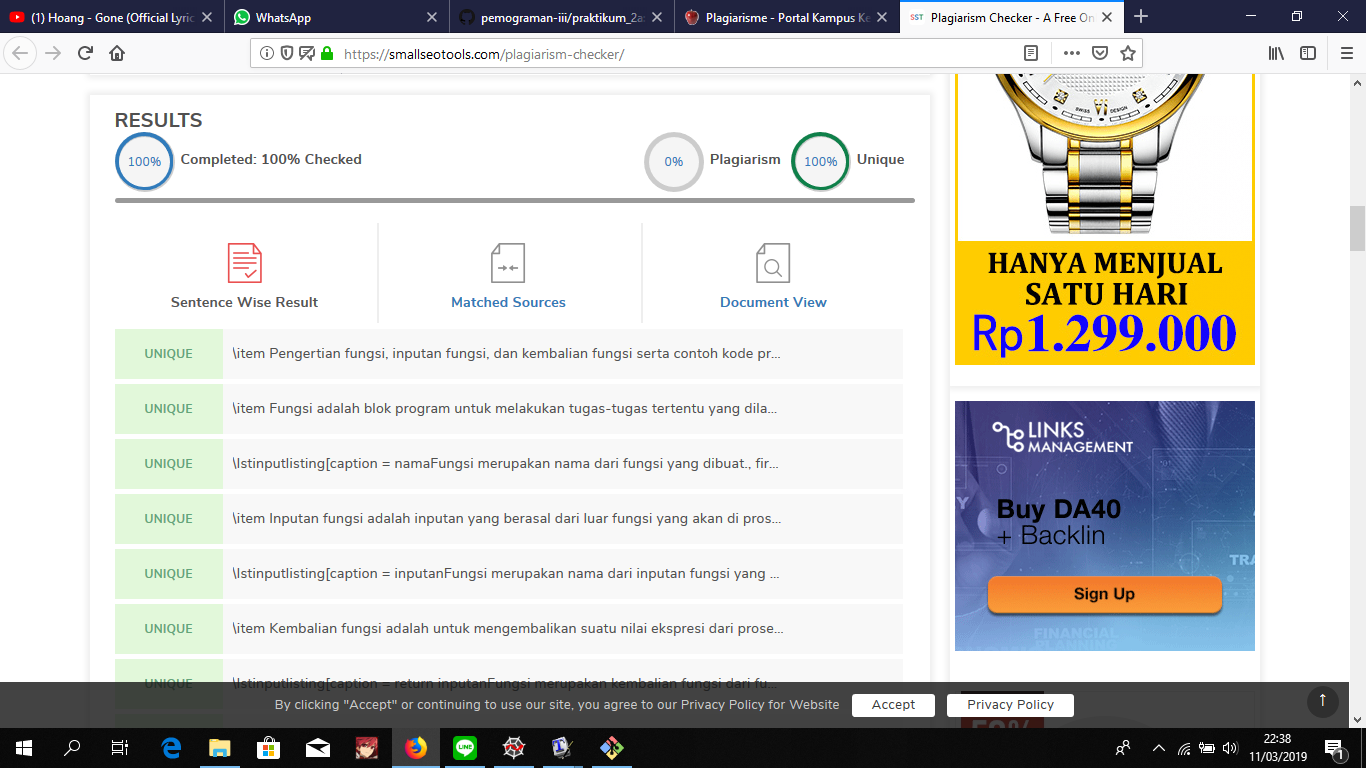
\includegraphics[width=6cm,height=6cm]{figures/habib.png}
\caption{SS Bebas Plagiarisme}
\label{habib}
\end{figure}
%%%%%%%%%%%%%%%%%%%%%%%%%%%%%%%%%%%%%%%%%%%%%%%%%%%%%%
%%%%%%%%%%%%%%%%%%%%%%%%%%%%%%%%%%%%%%%%%%%%%%%%%%%%%%
\section{Dezha Martha}
\subsection{Pemahaman Teori}
\begin{enumerate}
    \item Apa itu fungsi, inputan fungsi dan kembalian fungsi dengan contoh kode program lainnya.
Fungsi memiliki tujuan agar kita dapat memecah program besar menjadi sub-sub program yang lebih sederhana. Pada saat kita membutuhkan suatu fitur maka kita tinggal memanggil fungsi yang telah kita buat. Fungsi pada python dibuat dengan kata kunci def dan diikuti dengan nama fungsi yang kita buat seperti contoh dibawah :
 \lstinputlisting[firstline=10, lastline=10]{src/1174025/1174025.py}
Inputan fungsi merupakan masukan yang kita berikan pada program dan program akan menampilkan hasil dari inputan yang kita masukkan. contoh dari inputan fungsi sebagai berikut :
 \lstinputlisting[firstline=13, lastline=13]{src/1174025/1174025.py}
Pengembalian fungsi memiliki tujuan untuk mengembalikan nilai dari hasil yang telah di proses. Dalam hal ini menggunakan kata kunci return yang diikuti dengan nilai atau variabel yang akan dikembalikan.
 \lstinputlisting[firstline=11, lastline=11]{src/1174025/1174025.py}

    \item Apa itu paket dan cara pemanggilan paket atau library dengan contoh kode program lainnya.
Library atau paket adalah modul-modul yang menyusun python. Modul-modul tersebut ditulis oleh berbagai orang dari seluruh dunia dan memiliki fungsi masing-masing untuk melakukan suatu hal. contoh kode programnya adalah sebagai berikut :
 \lstinputlisting[firstline=16, lastline=18]{src/1174025/1174025.py}

    \item Jelaskan Apa itu kelas, apa itu objek, apa itu atribut, apa itu method dan contoh kode program lainnya masing-masing.
kelas adalah Prototype yang ditentukan oleh pengguna untuk objek yang mendefinisikan seperangkat atribut yang menjadi ciri objek kelas apa pun. Objek ialah instansiasi atau perwujudan dari sebuah kelas. Bila kelas adalah prototipenya, dan objek adalah barang jadinya. Atribut adalah data anggota (variabel kelas dan variabel contoh) dan metode, diakses melalui notasi titik. Sedangkan method fungsi yang didefinisikan di dalam suatu kelas.
 \lstinputlisting[firstline=19, lastline=41]{src/1174025/1174025.py}

    \item Jelaskan cara pemanggilan library kelas dari instansiasi dan pemakaiannya dengan contoh program lainnya.
cara pemanggilan  library kelas dari instansiasi dan pemakaiannya adalah dengan cara meng-import library yang ada di dalam satu folder dan menggunakan kode berikut :
 \lstinputlisting[firstline=42, lastline=52]{src/1174025/1174025.py}

    \item Jelaskan dengan contoh pemakaian paket dengan perintah from kalkulator import Penambahan disertai dengan contoh kode lainnya.
contoh kodenya adalah sebagai berikut :
 \lstinputlisting[firstline=53, lastline=58]{src/1174025/1174025.py}

    \item Jelaskan dengan contoh kodenya, pemakaian paket fungsi apabila file library ada di dalam folder.
 Pemakaian paket adalah perkumpulan fungsi-fungsi. contoh kodenya adalah sebagai berikut :
 \lstinputlisting[firstline=59, lastline=73]{src/1174025/1174025.py}

    \item Jelaskan dengan contoh kodenya, pemakaian paket kelas apabila file library ada di dalam folder.
 \lstinputlisting[firstline=75, lastline=84]{src/1174025/1174025.py}

\end{enumerate}

\subsection{Praktek}
\begin{enumerate}
    \item jawaban no 1
 \lstinputlisting[caption = Jawaban soal no 1.,firstline=90, lastline=126]{src/1174025/1174025.py}

    \item jawaban no 2
 \lstinputlisting[caption = Jawaban soal no 2.,firstline=128, lastline=133]{src/1174025/1174025.py}

    \item jawaban no 3
 \lstinputlisting[caption = Jawaban soal no 3.,firstline=136, lastline=144]{src/1174025/1174025.py}

    \item jawaban no 4
 \lstinputlisting[caption = Jawaban soal no 4.,firstline=145, lastline=150]{src/1174025/1174025.py}

    \item jawaban no 5
 \lstinputlisting[caption = Jawaban soal no 5.,firstline=152, lastline=157]{src/1174025/1174025.py}

    \item jawaban no 6
 \lstinputlisting[caption = Jawaban soal no 6.,firstline=159, lastline=165]{src/1174025/1174025.py}

    \item jawaban no 7
 \lstinputlisting[caption = Jawaban soal no 7.,firstline=167, lastline=173]{src/1174025/1174025.py}

    \item jawaban no 8
 \lstinputlisting[caption = Jawaban soal no 8.,firstline=175, lastline=180]{src/1174025/1174025.py}

    \item jawaban no 9
 \lstinputlisting[caption = Jawaban soal no 9.,firstline=184, lastline=190]{src/1174025/1174025.py}

    \item jawaban no 10
 \lstinputlisting[caption = Jawaban soal no 10.,firstline=192, lastline=208]{src/1174025/1174025.py}

    \item jawaban 11
 \lstinputlisting[caption = Jawaban soal no 11.,firstline=8, lastline=21]{src/1174025/main.py}
 
    \item jawaban 12
 \lstinputlisting[caption = Jawaban soal no 12.,firstline=24, lastline=40]{src/1174025/main.py}
\end{enumerate}

\subsection{Praktek}
\begin{enumerate}
    \item Peringatan error yang ada dan penjelasannya.
    
    \begin{itemize}
    	\item Syntax errors
    	syntax error adalah suatu keadaan saat kode yang dijalankan pada Python menagalami kesalahan penulisan, penempatan dll.
    	Solusi nya adalah dengan menemukan letak sumber masalah dan memperbaikinya.
    	
    	\item Zero Division Error
    	ZeroDivisionError adalah exceptions yang terjadi eksekusi program menghasilkan perhitungan matematika pembagian dengan angka nol (0). Solusiya adalah tidak membagi suatu yang hasilnya nol.
    	\item Name Error
    	NameError adalah exception yang terjadi saat kode melakukan eksekusi terhadap local name atau global name yang tidak terdefinisi. Solusi nya ialah memastikan variabel atau function yang dipanggil ada atau tidak salah ketik.
    	\item Type Error
    	TypeError adalah exception yang terjadi saat dilakukan eksekusi terhadapt suatu operasi atau fungsi dengan tipe objek yang tidak sesuai. Solusinya adalah mengkonversi variabelnya sesuai dengan tipe data yang akan digunakan.
    \end{itemize}
    
    Contoh fungsi yang menggunakan try except
 \lstinputlisting[caption = Penggunaan Try Except .,firstline=214, lastline=221]{src/1174025/1174025.py}

\end{enumerate} 
%%%%%%%%%%%%%%%%%%%%%%%%%%%%%%%%%%%%%%%%%%%%
\section{Damara Benedikta}
\subsection{Pemahaman Teori}
\begin{enumerate}
    \item Apa itu fungsi, inputan fungsi dan kembalian fungsi dengan contoh kode program lainnya.
Fungsi memiliki tujuan agar kita dapat memecah program besar menjadi sub-sub program yang lebih sederhana.pada masing-masing  fitur pada program dapat dibuat dalam satu fungsi. Pada saat kita membutuhkan suatu fitur maka kita tinggal memanggil fungsi yang telah kita buat. Fungsi pada python dibuat dengan menggunakan kata kunci def dan diikuti dengan nama fungsi yang telah kita buat seperti contoh dibawah ini :
 \lstinputlisting[firstline=10, lastline=10]{src/1174012/1174012.py}
Inputan fungsi merupakan masukan yang kita berikan pada program dan program akan menampilkan hasil dari inputan yang telah kita masukkan atau akan menampilkan hasil pada proses selanjutnya. contoh dari inputan fungsi sebagai berikut :
 \lstinputlisting[firstline=11, lastline=11]{src/1174012/1174012.py}
Pengembalian fungsi memiliki tujuan untuk mengembalikan nilai dari hasil yang telah di proses. Dalam hal ini menggunakan kata kunci return yang diikuti dengan nilai atau variabel yang akan dikembalikan.
 \lstinputlisting[firstline=10, lastline=14]{src/1174012/1174012.py}

    \item Apa itu paket dan cara pemanggilan paket atau library dengan contoh kode program lainnya.
Library atau paket adalah modul-modul yang menyusun python. Modul-modul tersebut ditulis oleh berbagai orang dari seluruh dunia dan memiliki fungsi masing-masing untuk melakukan suatu hal. contoh kode programnya adalah sebagai berikut :
 \lstinputlisting[firstline=17, lastline=18]{src/1174012/1174012.py}

    \item Jelaskan Apa itu kelas, apa itu objek, apa itu atribut, apa itu method dan contoh kode program lainnya masing-masing.
kelas adalah Prototype atau blueprint untuk menciptakan suatu object  yang mendefinisikan seperangkat atribut yang menjadi ciri objek kelas apa pun. Objek ialah instansiasi atau perwujudan dari sebuah kelas. Bila kelas adalah prototipenya, dan objek adalah hasil dari class jadinya. Atribut merupakan data dari anggota (variabel kelas, variabel contoh) dan metode, yang diakses dengan notasi titik. Sedangkan method fungsi yang didefinisikan di dalam suatu kelas.
 \lstinputlisting[firstline=21, lastline=40]{src/1174012/1174012.py}

    \item Jelaskan cara pemanggilan library kelas dari instansiasi dan pemakaiannya dengan contoh program lainnya.
cara pemanggilan  library kelas dari instansiasi dan pemakaiannya adalah dengan cara meng-import library yang ada di dalam satu folder dengan menggunakan kode berikut :
 \lstinputlisting[firstline=43, lastline=51]{src/1174012/1174012.py}

    \item Jelaskan dengan contoh pemakaian paket dengan perintah from kalkulator import Penambahan disertai dengan contoh kode lainnya.
contoh kodenya adalah sebagai berikut :
 \lstinputlisting[firstline=54, lastline=57]{src/1174012/1174012.py}

    \item Jelaskan dengan contoh kodenya, pemakaian paket fungsi apabila file library ada di dalam folder.
 Pemakaian paket adalah perkumpulan fungsi-fungsi. contoh kodenya adalah sebagai berikut :
 \lstinputlisting[firstline=60, lastline=73]{src/1174012/1174012.py}

    \item Jelaskan dengan contoh kodenya, pemakaian paket kelas apabila file library ada di dalam folder.
 \lstinputlisting[firstline=76, lastline=84]{src/1174012/1174012.py}

\end{enumerate}

\subsection{Praktek}
\begin{enumerate}
    \item jawaban no 1
 \lstinputlisting[firstline=87, lastline=121]{src/1174012/1174012.py}

    \item jawaban no 2
 \lstinputlisting[firstline=124, lastline=129]{src/1174012/1174012.py}

    \item jawaban no 3
 \lstinputlisting[firstline=132, lastline=139]{src/1174012/1174012.py}

    \item jawaban no 4
 \lstinputlisting[firstline=142, lastline=146]{src/1174012/1174012.py}

    \item jawaban no 5
 \lstinputlisting[firstline=149, lastline=153]{src/1174012/1174012.py}

    \item jawaban no 6
 \lstinputlisting[firstline=156, lastline=161]{src/1174012/1174012.py}

    \item jawaban no 7
 \lstinputlisting[firstline=164, lastline=169]{src/1174012/1174012.py}

    \item jawaban no 8
 \lstinputlisting[firstline=172, lastline=178]{src/1174012/1174012.py}

    \item jawaban no 9
 \lstinputlisting[firstline=181, lastline=186]{src/1174012/1174012.py}

    \item jawaban no 10
 \lstinputlisting[firstline=189, lastline=204]{src/1174012/1174012.py}

    \item jawaban 11
 \lstinputlisting[firstline=8, lastline=22]{src/1174012/main.py}
 \item jawaban 12
 \lstinputlisting[firstline=24, lastline=39]{src/1174012/main.py}
\end{enumerate}

\subsection{Ketrampilan Penanganan Error}
\begin{enumerate}
	\item Peringatan error yang ditemukan dan penjelasannya serta buat sebuah fungsi try except untuk menanggulangi error.
	
	Peringatan error di praktek ketiga ini, yaitu:
	\begin{itemize}
		\item Syntax Errors
		Syntax Errors adalah suatu keadaan saat kode python mengalami kesalahan penulisan. Solusinya adalah memperbaiki penulisan kode yang salah.
		
		\item Zero Division Error
		ZeroDivisonError adalah exceptions yang terjadi saat eksekusi program menghasilkan perhitungan matematika pembagian dengan angka nol (0). Solusinya adalah tidak membagi suatu yang hasilnya nol.
		
		\item Name Error
		NameError adalah exception yang terjadi saat kode melakukan eksekusi terhadap local name atau global name yang tidak terdefinisi. Solusinya adalah memastikan variabel atau function yang dipanggil ada atau tidak salah ketik.
		
		\item Type Error
		TypeError merupakan suatu exception yang terjadi saat akan mengeksekusi suatu operasi atau fungsi dengan type object yang tidak sesuai. Solusinya adalah mengkoversi varibelnya sesuai dengan tipe data yang akan digunakan.
	\end{itemize}
   \end{enumerate}

   \begin{figure}
   \centering
   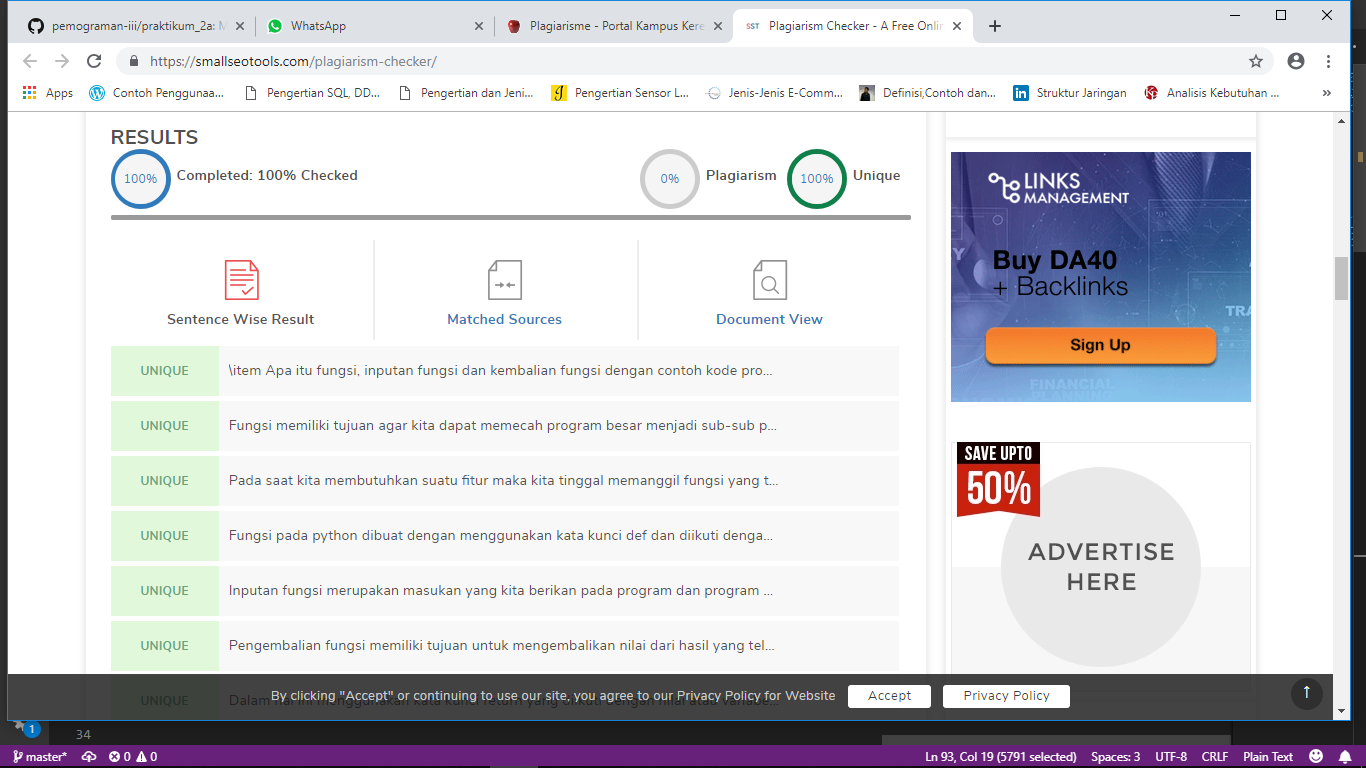
\includegraphics[width=6cm,height=6cm]{figures/damaraa.png}
   \caption{SS plagiarisme}
   \label{damara}
   \end{figure}

%%%%%%%%%%%%%%%%%%%%%%%%%%%%%%%%%%%%%%%%%%%%%%%%%%%%%%%%%%%%%%%%%%%%%%%%%%%

%%%%%%%%%%%%%%%%%%%%%%%%%%%%%%%%%%%%%%%%%%%%%%%%%%%%%%%%%%%%%%
\section{Arjun Yuda Firwanda}
\subsubsection{Pemahanan Teori}
\begin{enumerate}
    \item Apa itu fungsi, inputan fungsi dan kembalian fungsi dengan contoh kode program
    lainnya.
    Fungsi merupakan pendefinisian dengan kata kunci def dan diikuti parameter.
    \lstinputlisting[firstline=126, lastline=129]{src/1174008.py}

    Fungsi juga dapat membaca parameter, parameter adalah nilai yang disediakan kepada fungsi yang akan menentukan output yang akan dihasilkan fungsi.
    \lstinputlisting[firstline=131, lastline=134]{src/1174008.py}

    Perintah return digunakan untuk keluar dari fungsi. Kita juga dapat menspesifikasikan nilai kembalian.
    \lstinputlisting[firstline=136, lastline=143]{src/1174008.py}

    \item Apa itu paket dan cara pemanggilan paket atau library dengan contoh kode
    program lainnya.
    Paket untuk memudahkan dalam pemanggilan fungsi yang di butuhkan agar dapat dipanggil secara berulang.
    Cara pemanggilannya
    \lstinputlisting[firstline=145, lastline=146]{src/1174008.py}

    \item Jelaskan Apa itu kelas, apa itu objek, apa itu atribut, apa itu method dan
    contoh kode program lainnya masing-masing.
    Kelas merupakan blueprint cetakan atau kerangka dasar dari objek.
    Objek merupakan instance yang mempresentasikan nyata dari sebuah class.
    Method merupakan suatu operasi yang berupa fungsi-fungsi yang dikerjakan oleh sebuah objek.
    Attribute merupakan instan spesifik dari setiap objek.
    \lstinputlisting[firstline=148, lastline=170]{src/1174008.py}

    \item Jelaskan cara pemanggikan library kelas dari instansiasi dan pemakaiannya den-
    gan contoh program lainnya.
    Cara Pemanggilanya 
    \begin{itemize}
        \item pertama import terlebih dahulu filenya.
        \item kemudian buat variabel untuk menampung datanya.
        \item setelah itu panggil nama classnya dan panggil methodnya.
        \item Gunakan perintah print untuk menampilkan hasilnya.

    \end{itemize}
    \lstinputlisting[firstline=172, lastline=177]{src/1174008.py}

    \item Jelaskan dengan contoh pemakaian paket dengan perintah from kalkulator im-
    port Penambahan disertai dengan contoh kode lainnya.
    Penggunaan paket from namafile import yaitu berfungsi memanggil file dan fungsinya.
    \lstinputlisting[firstline=145, lastline=146]{src/1174008.py}

    \item Jelaskan dengan contoh kodenya, pemakaian paket fungsi apabila le library
    ada di dalam folder.
    Pemakaian paket merupakan sekumpulan fungsi-fungsi. contoh kodenya adalah sebagai berikut:

    \item Jelaskan dengan contoh kodenya, pemakaian paket kelas apabila le library ada
    di dalam folder.
    \lstinputlisting[firstline=186, lastline=186]{src/1174008.py}

\end{enumerate}
\subsubsection{Ketrampilan Pemrograman}
\begin{enumerate}
    \item Buatlah fungsi dengan inputan variabel NPM, dan melakukan print luaran huruf
    yang dirangkai dari tanda bintang, pagar atau plus dari NPM kita. Tanda
    bintang untuk NPM mod 3=0, tanda pagar untuk NPM mod 3 =1, tanda plus
    untuk NPM mod3=2.
    \lstinputlisting[firstline=186, lastline=236]{src/1174008.py}

    \item Buatlah fungsi dengan inputan variabel berupa NPM. kemudian dengan meng-
    gunakan perulangan mengeluarkan print output sebanyak dua dijit belakang
    NPM.
    \lstinputlisting[firstline=240, lastline=244]{src/1174008.py}

    \item Buatlah fungsi dengan dengan input variabel string bernama NPM dan beri
    luaran output dengan perulangan berupa tiga karakter belakang dari NPM se-
    banyak penjumlahan tiga dijit tersebut.
    \lstinputlisting[firstline=247, lastline=254]{src/1174008.py}

    \item Buatlah fungsi hello word dengan input variabel string bernama NPM dan
    beri luaran output berupa digit ketiga dari belakang dari variabel NPM meng-
    gunakan akses langsung manipulasi string pada baris ketiga dari variabel NPM.
    \lstinputlisting[firstline=257, lastline=260]{src/1174008.py}

    \item buat fungsi program dengan input variabel NPM dan melakukan print nomor npm satu persatu kebawah.
    \lstinputlisting[firstline=263, lastline=265]{src/1174008.py}

    \item Buatlah fungsi dengan inputan variabel NPM, didalamnya melakukan penjum-
    lahan dari seluruh dijit NPM tersebut, wajib menggunakan perulangan dan
    atau kondisi.
    \lstinputlisting[firstline=267, lastline=272]{src/1174008.py}

    \item Buatlah fungsi dengan inputan variabel NPM, didalamnya melakukan melakukan
    perkalian dari seluruh dijit NPM tersebut, wajib menggunakan perulangan dan
    atau kondisi.
    \lstinputlisting[firstline=274, lastline=279]{src/1174008.py}

    \item Buatlah fungsi dengan inputan variabel NPM, Lakukan print NPM anda tapi
    hanya dijit genap saja. wajib menggunakan perulangan dan atau kondisi.
    \lstinputlisting[firstline=281, lastline=286]{src/1174008.py}

    \item Buatlah fungsi dengan inputan variabel NPM, Lakukan print NPM anda tapi
    hanya dijit ganjil saja. wajib menggunakan perulangan dan atau kondisi.
    \lstinputlisting[firstline=288, lastline=293]{src/1174008.py}

    \item Buatlah fungsi dengan inputan variabel NPM, Lakukan print NPM anda tapi
    hanya dijit yang termasuk bilangan prima saja. wajib menggunakan perulangan
    dan atau kondisi.
    \lstinputlisting[firstline=295, lastline=308]{src/1174008.py}

    \item Buatlah satu library yang berisi fungsi-fungsi dari nomor diatas dengan nama
    le 3lib.py dan berikan contoh cara pemanggilannya pada le main.py.
    \lstinputlisting[firstline=7, lastline=7]{src/main.py}

    \item Buatlah satu library class dengan nama le kelas3lib.py yang merupakan mod-
    ikasi dari fungsi-fungsi nomor diatas dan berikan contoh cara pemanggilannya
    pada le main.py.
    \lstinputlisting[firstline=8, lastline=9]{src/main.py}
    
\end{enumerate}
\subsubsection{Ketrampilan Penanganan Error}
Error yang di dapat dari mengerjakan tugas ini adalah type error, cara menaggulaginya dengan cara mengecheck kembali codingannya
kemudian run kembali aplikasinya
berikut contoh Penggunaan fungsi try dan exception
\lstinputlisting[firstline=177, lastline=182]{src/1174008.py}



\section{Muhammad Fahmi}
\textbf{{\large Fungsi dan Kelas}}

\subsection{Pemahaman Teori}
\begin{enumerate}
	\item Fungsi adalah bagian dari program yang dapat digunakan ulang, kemudian nama ini dapat dipanggil di manapun dalam program.
	Contoh fungsi dan pemanggilannya adalah :
	\lstinputlisting[caption=Penggunaan fungsi, frame=single, firstline=3, lastline=6]{src/1174021/1174021.py}
	Fungsi juga dapat membaca parameter, parameter tersebut berupa nilai yang disediakan kepada fungsi, dimana nilai ini akan menentukan output yang akan dihasilkan fungsi. 
	\lstinputlisting[caption=Penggunaan fungsi,frame=single, firstline=8, lastline=12]{src/1174021/1174021.py}
	Didalam fungsi juga ada Statemen return yang digunakan untuk keluar dari fungsi. Kita juga dapat menspesifikasikan nilai kembalian.
	\lstinputlisting[caption=Penggunaan return,frame=single, firstline=14, lastline=21]{src/1174021/1174021.py}
	
	\item Paket didalam Python juga dikatakan Modul,  adalah sebuah file yang berisi kode python, misalnya: coba.py 
	Cara pemanggilan paket atau library yaitu dengan meng-import paket atau library yang akan digunakan. Kemudian panggil dengan cara mendefinisikan.
	\lstinputlisting[caption=Penggunaan paket atau library, frame=single, firstline=24, lastline=25]{src/1174021/1174021.py}
	
	\item \begin{itemize}
		\item Kelas
		Kelas adalah berupa blueprint atau cetak biru dari sebuah objek dimana kita mendefinisikan atribut dari suatu objek tersebut.
		Contoh penggunaan kelas adalah : 
		\lstinputlisting[caption = Penggunaan kelas di python, firstline=28, lastline=47]{src/1174021/1174021.py}
		
		\item Objek
		Objjek adalah sebuah contoh unik dari struktur data yang didefinisikan oleh kelasnya. Objek juga terdiri dari beberapa anggota data dan metode.
		\lstinputlisting[caption = Penggunaan objek di python, firstline=39, lastline=42]{src/1174021/1174021.py}
		
		\item Atribut
		Atribut adalah variabel yang menyimpan data yang berhubungan dengan kelas dan objeknya.
		\lstinputlisting[caption = Penggunaan atribut di python, firstline=29, lastline=29]{src/1174021/1174021.py}
		
		\item Method
		Methode atau moetode adalah sebuah jenis fungsi khusus yang didefinisikan dalam definisi kelas.
		\lstinputlisting[caption = Penggunaan method di python, firstline=35, lastline=37]{src/1174021/1174021.py}
		
	\end{itemize}
	
	
	\item Cara pemanggikan library kelas dari instansiasi dan pemakaiannya, berikut adalah contohnya : 
	\lstinputlisting[caption = Pemanggilan libraby kelas, firstline=50, lastline=60]{src/1174021/1174021.py}
	
	\item Pemakaian paket dengan perintah from kalkulator import Penambahan, berikut adalah contohnya : 
	\lstinputlisting[caption = Pemakaian paket from kalkulator import penambahan, firstline=63, lastline=66]{src/1174021/1174021.py}
	
	\item Pemakaian paket fungsi apabila file library ada di dalam folder, berikut adalah contohnya : 
	\lstinputlisting[caption = Pemakaian paket fungsi, firstline=69, lastline=82]{src/1174021/1174021.py}
	
	\item Pemakaian paket kelas apabila file library ada di dalam folder, berikut adalah contohnya : 
	\lstinputlisting[caption = Pemakaian paket fungsi2, firstline=85, lastline=95]{src/1174021/1174021.py}
	
\end{enumerate}

Hasil tampilan pemahaman teori : 
\begin{figure}[h]
	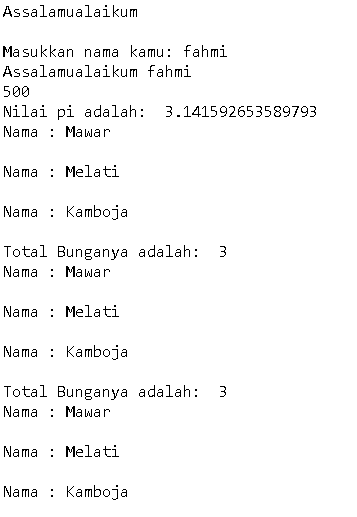
\includegraphics[width=50mm]{figures/fahmi/5.png}
	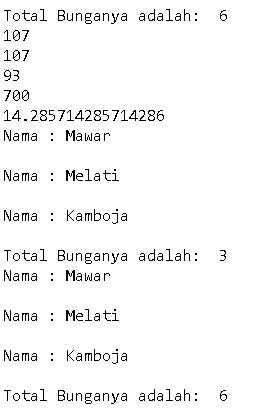
\includegraphics[width=50mm]{figures/fahmi/6.png}
	\centering
\end{figure}


\newpage
\subsection{Keterampilan Program}
\begin{enumerate}
	\item Jawaban Soal 1
	\lstinputlisting[caption = Jawaban Soal 1, firstline=101, lastline=146]{src/1174021/1174021.py}
	
	\item Jawaban Soal 2
	\lstinputlisting[caption = Jawaban Soal 2, firstline=149, lastline=157]{src/1174021/1174021.py}
	
	\item Jawaban Soal 3
	\lstinputlisting[caption = Jawaban Soal 3, firstline=160, lastline=168]{src/1174021/1174021.py}
	
	\item Jawaban Soal 4
	\lstinputlisting[caption = Jawaban Soal 4, firstline=171, lastline=177]{src/1174021/1174021.py}
	
	\item Jawaban Soal 5
	\lstinputlisting[caption = Jawaban Soal 5, firstline=180, lastline=187]{src/1174021/1174021.py}
	
	\item Jawaban Soal 6
	\lstinputlisting[caption = Jawaban Soal 6, firstline=190, lastline=197]{src/1174021/1174021.py}
		
	\item Jawaban Soal 7
	\lstinputlisting[caption = Jawaban Soal 7, firstline=200, lastline=207]{src/1174021/1174021.py}
	
	\item Jawaban Soal 8
	\lstinputlisting[caption = Jawaban Soal 8, firstline=210, lastline=217]{src/1174021/1174021.py}
	
	\item Jawaban Soal 9
	\lstinputlisting[caption = Jawaban Soal 9, firstline=220, lastline=228]{src/1174021/1174021.py}
	
	\item Jawaban Soal 10
	\lstinputlisting[caption = Jawaban Soal 9, firstline=231, lastline=248]{src/1174021/1174021.py}
	
	\item Jawaban Soal 11
	\lstinputlisting[caption = Jawaban Soal 9, firstline=1, lastline=3]{src/1174021/main.py}
	
	\item Jawaban Soal 12
	\lstinputlisting[caption = Jawaban Soal 9, firstline=7, lastline=11]{src/1174021/main.py}
	
\end{enumerate}

\subsection{Keterampilan Penanganan Error}
\begin{enumerate}
	\item Peringatan error yang ditemukan dan penjelasannya serta buat sebuah fungsi try except untuk menanggulangi error.
	
	Jenis-jenis error pada praktek kali ini adalah :
	\begin{itemize}
	\item Syntax Errors
	Syntax Errors adalah suatu keadaan dimana kode python mengalami kesalahan penulisan. Solusinya adalah memperbaiki penulisan kode yang salah.
	
	\item Zero Division Error
	ZeroDivisonError adalah sebuah exceptions yang terjadi saat kita mengeksekusi sebuah program kemudian menghasilkan perhitungan matematika pembagian dengan angka nol (0) solusinya adalah tidak membagi suatu yang hasilnya nol.
	
	\item Name Error
	NameError adalah sebuah exceptions yang terjadi jika sebuah kode melakukan eksekusi terhadap local name atau global name yang tidak terdefinisi. Solusinya adalah dengan memastikan variabel atau function yang telah dipanggil ada atau tidak salah ketik.
	
	\item Type Error
	TypeError adalah sebuah exceptions yang terjadi pada saat melakukan eksekusi terhadap suatu operasi atau fungsi dengan type object yang tidak sesuai. Solusinya adalah dengan mengkoversi varibelnya sesuai dengan tipe data yang akan digunakan.
	\end{itemize}
	
	Contoh fungsi yang menggunakan try except
	\lstinputlisting[caption= Fungsi yang menggunakan try except ,firstline=255, lastline=261]{src/1174021/1174021.py}
\end{enumerate}


\section{Muhammad Dzihan Al-Banna}
\subsection{Pemahaman Teori}
\subsubsection{Apa itu fungsi}
Fungsi adalah sebuah program yang dapat digunakan ulang. Sebuah fungsi dapat digunakan ulang dengan cara memberi nama pada blok statemen kemudian nama tersebut dapat dipanggil dalam program lain. 
\lstinputlisting[caption = contoh fungsi, firstline=8, lastline=11]{src/1174095/persib.py}
Inputan fungsi adalah sebuah fungsi yang mempunyai interkasi dengan user dan dapat menginputkan value.
\lstinputlisting[caption = contoh input fungsi, firstline=14, lastline=17]{src/1174095/persib.py}
Kembalian fungsi adalah hasil yang dikembalikan dari inputan.
\lstinputlisting[caption = contoh fungsi yang menghasilkan kembalian, firstline=20, lastline=127]{src/1174095/persib.py} 
\subsubsection{Apa itu paket}
Package adalah suatu teknik pengemasan modul di dalam python. Package menyediakan kemampuan bagi programmer untuk mengelompokkan modul yang telah dibuat. untuk pemanggilan sebuah package maka perlu dibuat dulu package yang akan dipanggil dan cara memanggilnya seperti berikut :
\lstinputlisting[caption = pakcage, firstline=28, lastline=31]{src/1174095/persib.py}

\subsubsection{Apa itu kelas, objek dan atribut}
kelas adalah Prototipe yang ditentukan oleh pengguna untuk sebuah objek yang mendefinisikan seperangkat atribut yang menjadi ciri objek kelas.
\lstinputlisting[caption = kelas python, firstline=32, lastline=49]{src/1174095/persib.py}
Atribut adalah data anggota dan metode,dapat diakses melalui notasi titik.
Objek adalah Contoh unik dari struktur yang didefinisikan oleh kelas. 
Objek terdiri dari kedua anggota data (variabel kelas dan variabel contoh) dan metode.
\lstinputlisting[caption = objek, firstline=43, lastline=44]{src/1174095/persib.py}
dan atribut seperti code di bawah ini :
\lstinputlisting[caption = atribut, firstline=49, lastline=49]{src/1174095/persib.py}
\subsubsection{pemanggilan library}
Dalam pemanggilan sebuah package ada langkah-langkah yang harus dikerjakan seperti langkah berikut ini :
\begin{enumerate}
	\item Import dahulu paket yang akan dipanggil
	\item buat variabel
	\item panggil method dan class
	\item buat print untuk menampilkan hasilnya
	print("Sepedanya ", Sepeda.jumlahSepeda)
	\lstinputlisting[caption = pemanggilan pakcage, firstline=52, lastline=60]{src/1174095/persib.py}
\end{enumerate}
\subsubsection{Pemakaian paket}
\lstinputlisting[caption = pemakaian package, firstline=62, lastline=62]{src/1174095/persib.py}
\subsubsection{Paket fungsi file di dalam folder}
\lstinputlisting[caption = pemanggilan file dalam folder, firstline=64, lastline=68]{src/1174095/persib.py}
\subsubsection{Paket kelas file di dalam folder}
\lstinputlisting[caption = pemakaian package kelas di luar folder, firstline=62, lastline=62]{src/1174095/persib.py}
\subsection{Keterampilan Pemrograman}
\begin{enumerate}
	\item Tugas 1
	\lstinputlisting[caption = tugas 1, firstline=9, lastline=43]{src/1174095/radovic.py}
	\begin{figure}
		
		\caption{}
	\end{figure}
	\item Tugas 2
	\lstinputlisting[caption = pemakaian package, firstline=46, lastline=51]{src/1174095/radovic.py}
	\item Tugas 3
	\lstinputlisting[caption = pemakaian package, firstline=54, lastline=61]{src/1174095/radovic.py}
	\item Tugas 4
	\lstinputlisting[caption = pemakaian package, firstline=64, lastline=68]{src/1174095/radovic.py}
	\item Tugas 5
	\lstinputlisting[caption = pemakaian package, firstline=71, lastline=75]{src/1174095/radovic.py}
	\item Tugas 6
	\lstinputlisting[caption = pemakaian package, firstline=78, lastline=83]{src/1174095/radovic.py}
	\item Tugas 7
	\lstinputlisting[caption = pemakaian package, firstline=86, lastline=91]{src/1174095/radovic.py}
	\item Tugas 8
	\lstinputlisting[caption = pemakaian package, firstline=94, lastline=100]{src/1174095/radovic.py}
	\item Tugas 9
	\lstinputlisting[caption = pemakaian package, firstline=103, lastline=108]{src/1174095/radovic.py}
	\item Tugas 10
	\lstinputlisting[caption = pemakaian package, firstline=112, lastline=127]{src/1174095/radovic.py}
	\item Tugas 11
	\lstinputlisting[caption = pemakaian package, firstline=1, lastline=3]{src/1174095/main.py}
	\item Tugas 12
	\lstinputlisting[caption = pemakaian package, firstline=5, lastline=9]{src/1174095/main.py}
\end{enumerate}
\subsection{Keterampilan Penanganan Error}
\begin{enumerate}
	\item Peringatan error yang ditemukan dan penjelasannya serta buat sebuah fungsi try except untuk menanggulangi error.
	
	Peringatan error di praktek ketiga ini, yaitu:
	\begin{itemize}
		\item Syntax Errors
		Syntax Errors adalah suatu keadaan disaat kode mengalami kesalahan penulisan. Cara menanganinya adalah dengan memperbaiki penulisan kode yang salah.
		
		\item Zero Division Error
		Zero Divison Error adalah exceptions yang terjadi saat eksekusi program menghasilkan perhitungan matematika pembagian dengan angka nol (0). Solusinya adalah tidak membagi suatu yang hasilnya nol.
		
		\item Name Error
		NameError adalah exception yang terjadi saat melakukan eksekusi terhadap local name atau global name yang tidak terdefinisi. Solusinya adalah memastikan bahwa variabel atau function yang dipanggil tidak salah penulisan.
		
		\item Type Error
		TypeError adalah exception yang terjadi saat melakukan eksekusi terhadap suatu operasi atau fungsi dengan type object yang tidak sesuai. Solusinya adalah mengkoversi varibelnya sesuai dengan tipe data yang akan digunakan.
		\lstinputlisting[caption = pemakaian package, firstline=131, lastline=137]{src/1174095/radovic.py}
	\end{itemize}
\end{enumerate}

\section{Hasil}
\begin{itemize}
	\item Hasil
	\begin{figure}[H]
		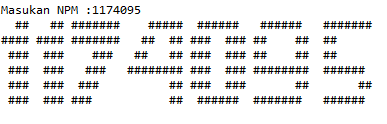
\includegraphics[width=10cm]{figures/dzihan/hasil.png}
		\centering
	\end{figure}
	\item Hasil 2
	\begin{figure}[H]
		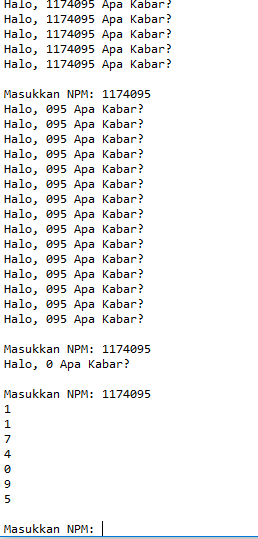
\includegraphics[width=10cm]{figures/dzihan/2f.png}
		\centering
	\end{figure}
	\item hasil 3
	\begin{figure}[H]
		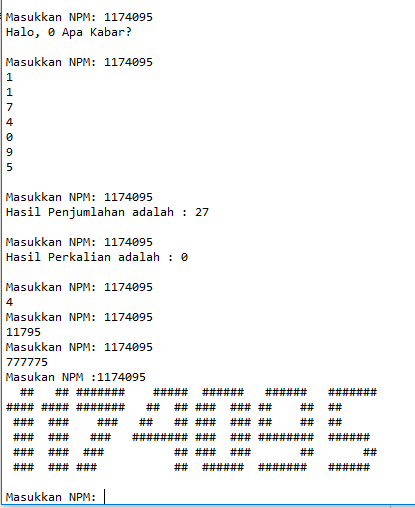
\includegraphics[width=10cm]{figures/dzihan/3.png}
		\centering
	\end{figure}
\end{itemize}

%%%%%%%%%%%%%%%%%%%%%%%%%
\section{Nico Ekklesia Sembiring}
\subsection{Tugas Teori}
\begin{enumerate}
	\item Apa itu fungsi, inputan fingsi dan kembalian fungsi dengan contoh kode program
	lainnya.\newline
	Fungsi merupakan suatu blok program yang terdiri atas nama fungsi, input variabel, dan kembalian variabel. 
	Fungsi pada python dibuat dengan kata kunci "def" dan diikuti dengan nama fungsi. contohnya adalah:
	\lstinputlisting[firstline=10, lastline=14]{src/1174096/1174096.py}
	
	\item Apa itu paket dan cara pemanggilan paket atau library dengan contoh kode program lainnya.\newline
	Library atau paket adalah modul-modul yang menyusun python. Modul-modul tersebut ditulis oleh berbagai orang dari seluruh dunia dan memiliki fungsi masing-masing untuk melakukan suatu hal. contoh kode programnya adalah sebagai berikut :
	\lstinputlisting[firstline=17, lastline=18]{src/1174096/1174096.py}
	
	\item Jelaskan Apa itu kelas, apa itu objek, apa itu atribut, apa itu method dan contoh kode program lainnya masing-masing.\newline
	Kelas adalah Prototype yang ditentukan oleh pengguna untuk objek yang mendefinisikan seperangkat atribut yang menjadi ciri objek kelas apa pun. Objek ialah instansiasi atau perwujudan dari sebuah kelas. Contoh dapat dilihat sebagai berikut :
	\lstinputlisting[firstline=21, lastline=39]{src/1174096/1174096.py}
	
	\item Jelaskan cara pemanggikan library kelas dari instansiasi dan pemakaiannya dengan contoh program lainnya.\newline
	Cara pemanggilan  library kelas dari instansiasi dan pemakaiannya adalah dengan cara meng-import library yang ada di dalam satu folder dan menggunakan kode berikut :
	\lstinputlisting[firstline=42, lastline=50]{src/1174096/1174096.py}
	
	\item Jelaskan dengan contoh pemakaian paket dengan perintah from kalkulator import Penambahan disertai dengan contoh kode lainnya.\newline
	Penggunaan paket dengan perintah from kalkulator berfungsi untuk memanggil file dan fungsinya. contoh kodenya adalah sebagai berikut :
	\lstinputlisting[firstline=53, lastline=56]{src/1174096/1174096.py}
	
	\item Jelaskan dengan contoh kodenya, pemakaian paket fungsi apabila file library ada di dalam folder.\newline
	Pemakaian paket adalah perkumpulan fungsi-fungsi. contoh kodenya adalah sebagai berikut :
	\lstinputlisting[firstline=59, lastline=72]{src/1174096/1174096.py}
	
	\item Jelaskan dengan contoh kodenya, pemakaian paket kelas apabila file library ada
	di dalam folder.\newline
	\lstinputlisting[firstline=75, lastline=83]{src/1174096/1174096.py}
\end{enumerate}

\subsection{Tugas Keterampilan Pemrograman}
\begin{enumerate}
	\item Buatlah fungsi dengan inputan variabel NPM, dan melakukan print luaran huruf yang dirangkai dari tanda bintang, pagar atau plus dari NPM kita. Tanda bintang untuk NPM mod 3=0, tanda pagar untuk NPM mod 3 =1, tanda plus untuk NPM mod3=2.
	\lstinputlisting[firstline=89, lastline=123]{src/1174096/1174096.py}
	
	\item Buatlah fungsi dengan inputan variabel berupa NPM. kemudian dengan menggunakan perulangan mengeluarkan print output sebanyak dua dijit belakang
	NPM.
	\lstinputlisting[firstline=126, lastline=131]{src/1174096/1174096.py}
	
	\item Buatlah fungsi dengan dengan input variabel string bernama NPM dan beri
	luaran output dengan perulangan berupa tiga karakter belakang dari NPM sebanyak penjumlahan tiga dijit tersebut. Penjumlahan dilakukan dengan menggunakan operator aritmatika dan fungsi int() atau str().
	\lstinputlisting[firstline=134, lastline=141]{src/1174096/1174096.py}
	
	\item Buatlah fungsi hello word dengan input variabel string bernama NPM dan beri luaran output berupa digit ketiga dari belakang dari variabel NPM menggunakan akses langsung manipulasi string pada baris ketiga dari variabel NPM.
	\lstinputlisting[firstline=144, lastline=148]{src/1174096/1174096.py}
	
	\item Buat fungsi program dengan input variabel NPM dan melakukan print nomor npm satu persatu kebawah.
	\lstinputlisting[firstline=151, lastline=155]{src/1174096/1174096.py}
	
	\item Buatlah fungsi dengan inputan variabel NPM, didalamnya melakukan penjumlahan dari seluruh dijit NPM tersebut, wajib menggunakan perulangan dan
	atau kondisi.
	\lstinputlisting[firstline=158, lastline=163]{src/1174096/1174096.py}
	
	\item Buatlah fungsi dengan inputan variabel NPM, didalamnya melakukan melakukan perkalian dari seluruh dijit NPM tersebut, wajib menggunakan perulangan dan atau kondisi.
	\lstinputlisting[firstline=166, lastline=171]{src/1174096/1174096.py}
	
	\item Buatlah fungsi dengan inputan variabel NPM, Lakukan print NPM anda tapi hanya dijit genap saja. wajib menggunakan perulangan dan atau kondisi
	\lstinputlisting[firstline=174, lastline=180]{src/1174096/1174096.py}
	
	\item Buatlah fungsi dengan inputan variabel NPM, Lakukan print NPM anda tapi hanya dijit ganjil saja. wajib menggunakan perulangan dan atau kondisi..
	\lstinputlisting[firstline=183, lastline=188]{src/1174096/1174096.py}
	
	\item Buatlah fungsi dengan inputan variabel NPM, Lakukan print NPM anda tapi hanya dijit yang termasuk bilangan prima saja. wajib menggunakan perulangan dan atau kondisi..
	\lstinputlisting[firstline=191, lastline=206]{src/1174096/1174096.py}
	
	\item Buatlah satu library yang berisi fungsi-fungsi dari nomor diatas dengan nama file 3lib.py dan berikan contoh cara pemanggilannya pada file main.py.
	\lstinputlisting[firstline=8, lastline=21]{src/1174096/main.py}
	
	\item Buatlah satu library class dengan nama file kelas3lib.py yang merupakan modifikasi dari fungsi-fungsi nomor diatas dan berikan contoh cara pemanggilannya pada file main.py..
	\lstinputlisting[firstline=23, lastline=38]{src/1174096/main.py}
	
\end{enumerate}
\subsection{Ketrampilan Penanganan Error}
\lstinputlisting[firstline=209, lastline=214]{src/1174096/1174096.py}

\subsection{Cek Plagiarisme}
\begin{figure}[!htbp]
	\centering
	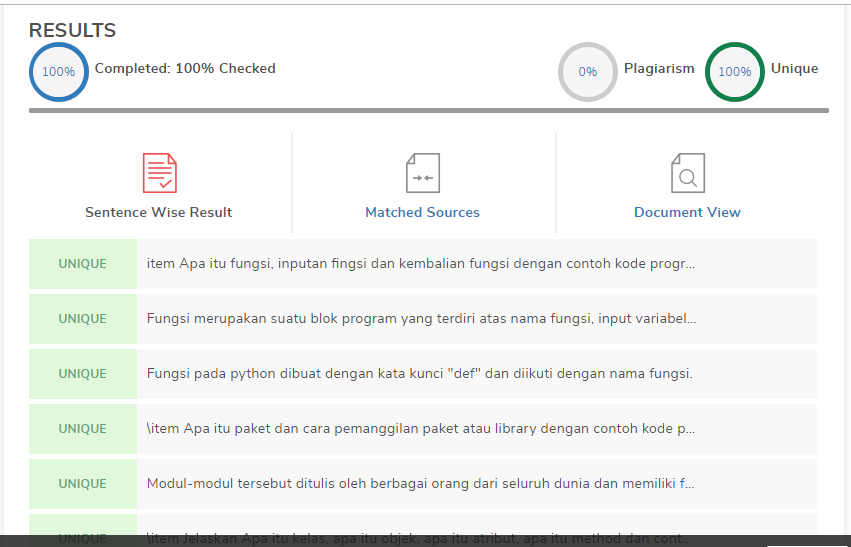
\includegraphics[width=3cm,height=3cm]{figures/nico/plagiarisme.png}
	\caption{Plagiarisme}
	\label{plagiarisme}
\end{figure}

%%%%%%%%%%%%%%%%%%%%%%%%%%%%%

\section{Oniwaldus Bere Mali}
\subsection{Tugas Teori}
\begin{enumerate}
\item Apa itu fungsi, inputan fingsi dan kembalian fungsi dengan contoh kode program
lainnya.\newline
Fungsi merupakan suatu blok program yang terdiri atas nama fungsi, input variabel, dan kembalian variabel. 
Fungsi pada python dibuat dengan kata kunci "def" dan diikuti dengan nama fungsi. contohnya adalah:
\lstinputlisting[firstline=10, lastline=14]{src/1174005/1174005.py}

\item Apa itu paket dan cara pemanggilan paket atau library dengan contoh kode program lainnya.\newline
Library atau paket adalah modul-modul yang menyusun python. Modul-modul tersebut ditulis oleh berbagai orang dari seluruh dunia dan memiliki fungsi masing-masing untuk melakukan suatu hal. contoh kode programnya adalah sebagai berikut :
\lstinputlisting[firstline=17, lastline=18]{src/1174005/1174005.py}

\item Jelaskan Apa itu kelas, apa itu objek, apa itu atribut, apa itu method dan contoh kode program lainnya masing-masing.\newline
Kelas adalah Prototype yang ditentukan oleh pengguna untuk objek yang mendefinisikan seperangkat atribut yang menjadi ciri objek kelas apa pun. Objek ialah instansiasi atau perwujudan dari sebuah kelas. Contoh dapat dilihat sebagai berikut :
\lstinputlisting[firstline=21, lastline=39]{src/1174005/1174005.py}

\item Jelaskan cara pemanggikan library kelas dari instansiasi dan pemakaiannya dengan contoh program lainnya.\newline
Cara pemanggilan  library kelas dari instansiasi dan pemakaiannya adalah dengan cara meng-import library yang ada di dalam satu folder dan menggunakan kode berikut :
\lstinputlisting[firstline=42, lastline=50]{src/1174005/1174005.py}

\item Jelaskan dengan contoh pemakaian paket dengan perintah from kalkulator import Penambahan disertai dengan contoh kode lainnya.\newline
Penggunaan paket dengan perintah from kalkulator berfungsi untuk memanggil file dan fungsinya. contoh kodenya adalah sebagai berikut :
\lstinputlisting[firstline=53, lastline=56]{src/1174005/1174005.py}

\item Jelaskan dengan contoh kodenya, pemakaian paket fungsi apabila file library ada di dalam folder.\newline
Pemakaian paket adalah perkumpulan fungsi-fungsi. contoh kodenya adalah sebagai berikut :
\lstinputlisting[firstline=59, lastline=72]{src/1174005/1174005.py}

\item Jelaskan dengan contoh kodenya, pemakaian paket kelas apabila file library ada
di dalam folder.\newline
\lstinputlisting[firstline=75, lastline=83]{src/1174005/1174005.py}
\end{enumerate}

\subsection{Tugas Keterampilan Pemrograman}
\begin{enumerate}
\item Buatlah fungsi dengan inputan variabel NPM, dan melakukan print luaran huruf yang dirangkai dari tanda bintang, pagar atau plus dari NPM kita. Tanda bintang untuk NPM mod 3=0, tanda pagar untuk NPM mod 3 =1, tanda plus untuk NPM mod3=2.
    \lstinputlisting[firstline=89, lastline=123]{src/1174005/1174005.py}

\item Buatlah fungsi dengan inputan variabel berupa NPM. kemudian dengan menggunakan perulangan mengeluarkan print output sebanyak dua dijit belakang
NPM.
    \lstinputlisting[firstline=126, lastline=131]{src/1174005/1174005.py}
    
\item Buatlah fungsi dengan dengan input variabel string bernama NPM dan beri
luaran output dengan perulangan berupa tiga karakter belakang dari NPM sebanyak penjumlahan tiga dijit tersebut. Penjumlahan dilakukan dengan menggunakan operator aritmatika dan fungsi int() atau str().
    \lstinputlisting[firstline=134, lastline=141]{src/1174005/1174005.py}

\item Buatlah fungsi hello word dengan input variabel string bernama NPM dan beri luaran output berupa digit ketiga dari belakang dari variabel NPM menggunakan akses langsung manipulasi string pada baris ketiga dari variabel NPM.
    \lstinputlisting[firstline=144, lastline=148]{src/1174005/1174005.py}

\item Buat fungsi program dengan input variabel NPM dan melakukan print nomor npm satu persatu kebawah.
    \lstinputlisting[firstline=151, lastline=155]{src/1174005/1174005.py}

\item Buatlah fungsi dengan inputan variabel NPM, didalamnya melakukan penjumlahan dari seluruh dijit NPM tersebut, wajib menggunakan perulangan dan
atau kondisi.
    \lstinputlisting[firstline=158, lastline=163]{src/1174005/1174005.py}

\item Buatlah fungsi dengan inputan variabel NPM, didalamnya melakukan melakukan perkalian dari seluruh dijit NPM tersebut, wajib menggunakan perulangan dan atau kondisi.
    \lstinputlisting[firstline=166, lastline=171]{src/1174005/1174005.py}

\item Buatlah fungsi dengan inputan variabel NPM, Lakukan print NPM anda tapi hanya dijit genap saja. wajib menggunakan perulangan dan atau kondisi
    \lstinputlisting[firstline=174, lastline=180]{src/1174005/1174005.py}

\item Buatlah fungsi dengan inputan variabel NPM, Lakukan print NPM anda tapi hanya dijit ganjil saja. wajib menggunakan perulangan dan atau kondisi..
    \lstinputlisting[firstline=183, lastline=188]{src/1174005/1174005.py}

\item Buatlah fungsi dengan inputan variabel NPM, Lakukan print NPM anda tapi hanya dijit yang termasuk bilangan prima saja. wajib menggunakan perulangan dan atau kondisi..
    \lstinputlisting[firstline=191, lastline=206]{src/1174005/1174005.py}

\item Buatlah satu library yang berisi fungsi-fungsi dari nomor diatas dengan nama file 3lib.py dan berikan contoh cara pemanggilannya pada file main.py.
    \lstinputlisting[firstline=8, lastline=21]{src/1174005/main.py}

\item Buatlah satu library class dengan nama file kelas3lib.py yang merupakan modifikasi dari fungsi-fungsi nomor diatas dan berikan contoh cara pemanggilannya pada file main.py..
    \lstinputlisting[firstline=23, lastline=38]{src/1174005/main.py}

\end{enumerate}
\subsection{Ketrampilan Penanganan Error}
   \lstinputlisting[firstline=209, lastline=214]{src/1174005/1174005.py}
   
\subsection{Cek Plagiarisme}
\begin{figure}[!htbp]
	\centering
	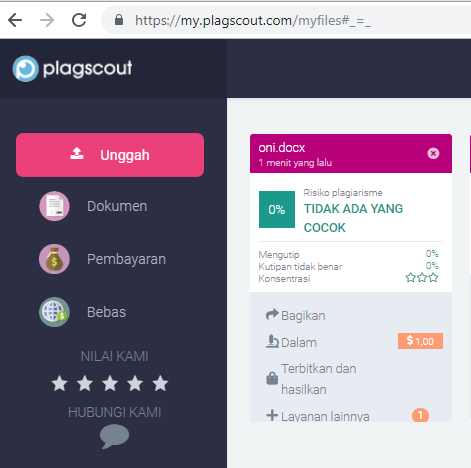
\includegraphics[width=3cm,height=3cm]{figures/oni/plagiarisme.png}
	\caption{Plagiarisme}
	\label{plagiarisme}
\end{figure}

\chapter{Kelompok 1}
\section{Harun Ar - Rasyid}
\begin{enumerate}
    \item Apa itu fungsi file csv, jelaskan sejarah dan contoh
    File CSV (Nilai Terbatas Koma) adalah jenis file khusus yang dapat Anda buat atau edit di Excel. File CSV menyimpan informasi yang dipisahkan oleh koma, tidak menyimpan informasi dalam kolom. Ketika teks dan angka disimpan dalam file CSV, mudah untuk memindahkannya dari satu program ke program lainnya.
    Dari rilis pertama, Excel menggunakan format file biner yang disebut Binary Interchange File Format (BIFF) sebagai format file utamanya. Ini berubah ketika Microsoft merilis Office System 2007 yang memperkenalkan Office Open XML sebagai format file utamanya. Office Open XML adalah file kontainer berbasis XML yang mirip dengan XML Spreadsheets (XMLSS), yang diperkenalkan di Excel 2002. File versi XML tidak bisa menyimpan makro VBA.
    Meskipun mendukung format XML baru, Excel 2007 masih mendukung format lama yang masih berbasis BIFF tradisional. Selain itu Microsoft Excel juga mendukung format Comma Separated Values (CSV), DBase File (DBF), SYMbolic LinK (SYLK), Format Interchange Data (DIF) dan banyak format lainnya, termasuk format lembar kerja 1-2 Lotus - 3 (WKS, WK1, WK2, dll.) Dan Quattro Pro.
    \item Aplikasi-aplikasi apa saja yang bisa menciptakan file csv
    \begin{itemize}
        \item Texteditor
        Seperti notepad++,visual studio code,atom,sublime dan lain sebagainya
        \item Program Spreadsheet
        Seperti excell,google spreadshare,LibreOfficecalc
    \end{itemize}
    \item Jelaskan bagaimana cara menulis dan membaca file csv di excel atau spreadsheet
    Untuk menulisnya untuk yang paling atas itu kita buat headernya,untuk mepermudah membedakan datanya,dan untuk baris kedua dan seterusnya itu untuk data itu sendiri.
    dan setelah di buat kalian save as kemudian pilih format CSV.
    dan untuk membukan cukup di double clik file tersebut
    \item Jelaskan sejarah library csv
    library csv dibuat untuk permudah mengolah data. Dan mempermudah untuk melakukan export dan import file csv itu sendiri
    \item Jelaskan sejarah library pandas
    library pandas dibuat agar bahasa pemograman python bisa bersaing R dan matlab, yang digunakan untuk mengolah banyak data , keperluan big data, data mining data science dan sebagainya.
    \item Jelaskan fungsi-fungsi yang terdapat di library csv
    Terdapat 2 fungsi yang bisa digunakan oleh library csv
    Pertama,fungsi membaca file csv.
    fungsi ini bisa menggunakan list dan dictionary
    Dengan list :
    \lstinputlisting[firstline=11, lastline=21]{src/1174027/1174027_csv.py}
    Dengan dictionary :
    \lstinputlisting[firstline=24, lastline=33]{src/1174027/1174027_csv.py}
    Kedua,fungsi menulis file csv.
    \lstinputlisting[firstline=36, lastline=40]{src/1174027/1174027_csv.py}
    \item Jelaskan fungsi-fungsi yang terdapat di library pandas
    Hampir sama dengan library csv,tp library pandas penulisannya lebih sederhana dan terlihat lebih rapih dari pada library csv.
    \lstinputlisting[firstline=43, lastline=44]{src/1174027/1174027_csv.py}
\end{enumerate}
%%%%%%%%%%%%%%%%%%%%%%%%%%%%%%%%%%%%%%%%%%%%%%%%%%%%%%%%

\section{Dwi Yulianingsih}
\subsection{Pemahaman Materi}
\begin{enumerate}
\item Apa itu fungsi file csv, jelaskan sejarah dan contoh
\paragraph{} CSV (Comma Separated Value) adalah format basis data sederhana yang dimana setiap record yang ada dipisahkan dengan tanda koma (,) atau titik koma (;). Format data file csv dapat diolah dengan berbagai text editor dengan mudah. Anda tidak perlu (dan Anda tidak akan) membuat pengurai CSV Anda sendiri dari awal. Ada beberapa perpustakaan yang dapat diterima yang dapat Anda gunakan. Pustaka csv Python akan berfungsi untuk sebagian besar kasus. Jika pekerjaan Anda memerlukan banyak data atau analisis numerik, panda library juga memiliki kemampuan penguraian CSV, yang seharusnya menangani sisanya. Dalam bahasa pemrograman Python telah disediakan modul csv yang khusus untuk mengolah data berformat csv.  Untuk memanipulasi data csv dengan python tentunya yang pertama dilakukan adalah mengimport modul csv dengan perintah import csv. File CSV biasanya dibuat oleh program yang menangani sejumlah besar data. Mereka adalah cara yang nyaman untuk mengekspor data dari spreadsheet dan basis data serta mengimpor atau menggunakannya dalam program lain. Misalnya, Anda dapat mengekspor hasil program penambangan data ke file CSV dan kemudian mengimpornya ke dalam spreadsheet untuk menganalisis data, menghasilkan grafik untuk presentasi, atau menyiapkan laporan untuk publikasi. Contoh nya adalah sebagai berikut :

 \lstinputlisting[firstline=8, lastline=20]{src/1174009/dudul.py}

\item Aplikasi-aplikasi apa saja yang bisa menciptakan file csv?
\paragraph{} Ada beberapa aplikasi yang dapat menciptakan file dengan format csv diantaranya google sheet, number di MacOS dan microsoft excel.
\subsection{Membuat dan membaca csv di excel atau spreadsheet}

\item Jelaskan bagaimana cara menulis dan membaca file csv di excel atau spreadsheet
\paragraph{} Cara membuat file csv di excel cukup mudah yaitu :
\begin{itemize}
	\item Buat foldernya
	\item Pilih save as
	\item pilih file dengan format csv
\end{itemize}
Cara membaca file di csv :
\begin{itemize}
	\item Klik data - get external data - form text
	\item Akan muncul Text Import Wizard, arahkan pada file csv yang ingin anda buka lalu Open.
	\item Setelah File terbuka, akan muncul Text Import Wizard.
	\item Pilih Delimited, Kemudian Next (Di sini, bisa juga menentukan baris awal yang akan di import)
	\item Centrang pada Tab dan Comma (Atau sesuai pengaturan File Anda) lalu Next.
	\item Atur Format data pada tiap kolom yang tampil dan klik Finish
\end{itemize}

\item Jelaskan sejarah library csv
\paragraph{} CSV muncul untuk memudahkan data science dan analis karena dinilai terdapat banyak kemudahan yang didapat. CSV dapat dimaksimalkan jika dipaduka dengan python karena python adalah bahasa pemrograman yang support ke banyak library termasuk csv. Maka karena itulah perpaduan python dan csv seringkali digunakan oleh perusahaan-perushaan besar dalam mengolah datanya.

\item Jelaskan sejarah library pandas
\paragraph{} Pandas merupakan tool yang dapat digunakan sebagai alat analisis data dan struktur untuk bahasa pemrograman Python. Pandas dapat mengolah data dengan mudah, salah satu fitur yang ada dalam pandas adalah Dataframe. Fitur dataframe dapat membaca sebuah file dan menjadikannya tabble, juga dapat mengolah suatu data dengan menggunakan operasi seperti join, group by dan teknik lainnya yang terdapat pada SQL. Dalam hal ini pandas tidak jauh beda dengan csv yaitu memiliki keunggulan dalam pengolahan data-data besar dan dapat disupport dengan baik dengan python walaupun mengimport data dalam jumlah banyak.

\item Jelaskan fungsi-fungsi yang terdapat di library csv
\paragraph{} Library csv mempunyai keunggulan dibandingkan format data lainnya adalah soal kompatibilitas. File csv dapat digunakan, diolah, diekspor/impor, dan dimodifikasi menggunakan berbagai macam perangkat lunak dan bahasa pemrograman. Pada library csv mempunyai fungsi import dan eksport data yang baik dan bisa digunakan dalam jumlah besar.

\item Jelaskan fungsi-fungsi yang terdapat di library pandas
\paragraph{} pandas menyediakan beragam fungsi operasi untuk mengolah data. Contoh jika menggunakan series bisa mencari nilai max, min, dan mean secara langsung, bahkan juga bisa melakukan operasi perpangkatan pada nilai Series secara langsung.
Pandas dapat mengolah suatu data dan mengolahnya seperti join, distinct, group by, agregasi, dan teknik seperti pada SQL. Hanya saja dilakukan pada tabel yang dimuat dari file ke RAM.
\end{enumerate}

\subsection{bukti bebas plagiarisme}
\begin{figure}[H]
\centering
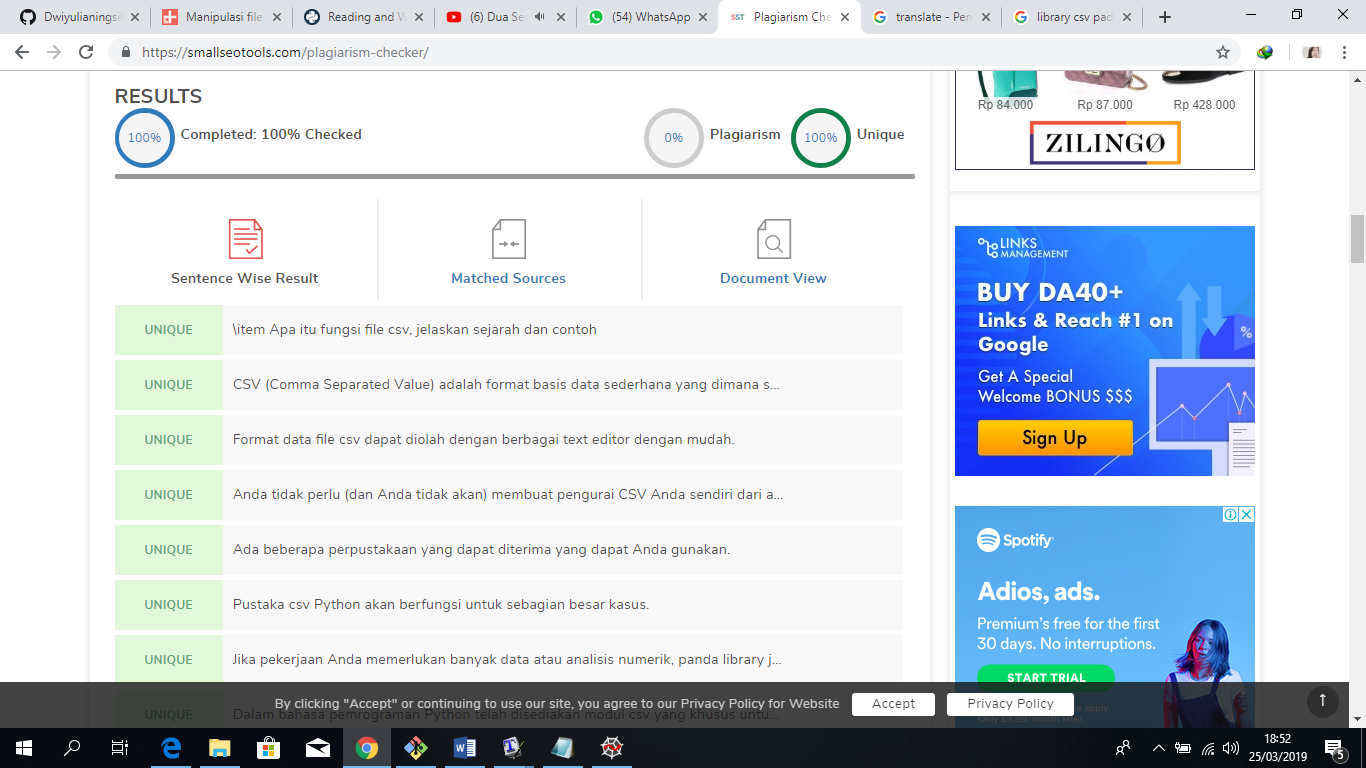
\includegraphics[width=10cm]{figures/yuli.png}
\caption{SS Bebas Plagiarisme}
\label{dwiyul}
\end{figure}
%%%%%%%%%%%%%%%%%%%%%%%%%%%%%%%%%%%%%%%%%%%%%%%%%%%%%%%%

\section{Muhammad Dzihan Al-Banna}
\subsection{Sejarah Csv}
\paragraph{}Comma Separated Value atau CSV adalah format data yang memudahkan penggunanya melakukan input data ke database secara sederhana. CSV dapat digunakan dalam standar file ASCII. Dalam format csv record dipisahkan dengan tanda koma atau titik koma. Ketika user menerima file dengan format CSV, yang biasanya bertuliskan .CSV, maka file tersebut akan terbuka dalam format Microsoft Excel. CSV muncul demi memenuhi kebutuhan perusahaan-perusahaan besar dalam mengolah data yang banyak.
\lstinputlisting[firstline=7, lastline=20]{src/1174095/cobacsv.py}
\subsubsection{Fungsi CSV}
\paragraph{}Fungsi csv yaitu memudahkan user dalam melakukan input data karena di csv input data atau import data dalam skala besar dapat dilakukan dengan cara yang sederhana.
\subsection{Aplikasi yang dapat menghasilkan csv}
\paragraph{}Ada beberapa aplikasi yang dapat menghasilkan file dengan format csv diantaranya google sheet, number di MacOS dan microsoft excel.
\subsection{Membuat dan membaca csv di excel atau spreadsheet}
\subsubsection{Membuat dan membaca csv di excel}
cara membuat file csv di excel cukup mudah yaitu :
\begin{itemize}
	\item Buat foldernya
	\item Pilih save as
	\item pilih file dengan format csv
\end{itemize}
cara membaca file di csv :
\begin{itemize}
	\item Klik data get external data form text
	\item Akan muncul Text Import Wizard, arahkan pada file csv yang ingin anda buka Open.
	\item Setelah File terbuka, akan muncul Text Import Wizard.
	\item Pilih Delimited, Kemudian Next (Di sini, bisa juga menentukan baris awal yang akan di import)
	\item Centrang pada Tab dan Comma (Atau sesuai pengaturan File Anda) Next.
	\item Atur Format data pada tiap kolom yang tampil dan klik Finish
\end{itemize}
\subsection{Sejarah Library CSV}
\paragraph{}CSV muncul untuk memudahkan data science dan analis karena dinilai terdapat banyak kemudahan yang didapat. CSV dapat dimaksimalkan jika dipaduka dengan python karena python adalah bahasa pemrograman yang support ke banyak library termasuk csv. Maka karena itulah perpaduan python dan csv seringkali digunakan oleh perusahaan-perushaan besar dalam mengolah datanya.
\subsection{Sejarah Library Pandas}
\paragraph{}Pandas merupakan tool yang dapat digunakan sebagai alat analisis data dan struktur untuk bahasa pemrograman Python. Pandas dapat mengolah data dengan mudah, salah satu fitur yang ada dalam pandas adalah Dataframe. Fitur dataframe dapat membaca sebuah file dan menjadikannya tabble, juga dapat mengolah suatu data dengan menggunakan operasi seperti join, group by dan teknik lainnya yang terdapat pada SQL. Dalam hal ini pandas tidak jauh beda dengan csv yaitu memiliki keunggulan dalam pengolahan data-data besar dan dapat disupport dengan baik dengan python walaupun mengimport data dalam jumlah banyak.
\subsection{Fungsi-fungsi Library CSV}
\paragraph{}Dalam library csv terdapat dua fungsi yaiut fungsi membaca file dan menulis file csv.
Library csv mempunyai keunggulan dibandingkan format data lainnya adalah soal kompatibilitas. File csv dapat digunakan, diolah, diekspor/impor, dan dimodifikasi menggunakan berbagai macam perangkat lunak dan bahasa pemrograman. Pada library csv mempunyai fungsi import dan eksport data yang baik dan bisa digunakan dalam jumlah besar.
\subsection{Fungsi-fungsi library Pandas}
\paragraph{}Pandas pun memiliki fungsi yang sama yaitu menulis dan membaca file. pandas menyediakan beragam fungsi operasi untuk mengolah data. Contoh jika menggunakan series bisa mencari nilai max, min, dan mean secara langsung, bahkan juga bisa melakukan operasi perpangkatan pada nilai Series secara langsung.
Pandas dapat mengolah suatu data dan mengolahnya seperti join, distinct, group by, agregasi, dan teknik seperti pada SQL. Hanya saja dilakukan pada tabel yang dimuat dari file ke RAM.
\subsection{Bukti Plagiarisme}
\begin{figure}[h]
	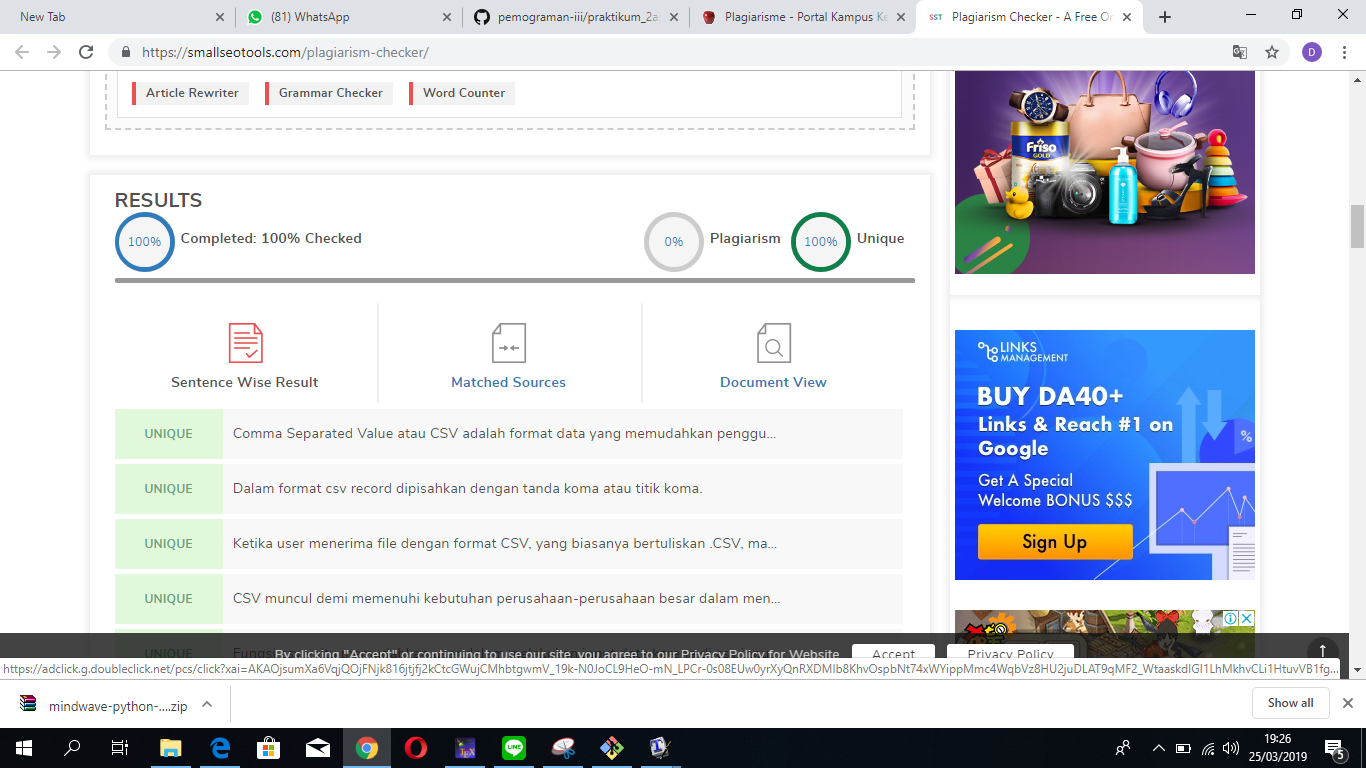
\includegraphics[width=10cm]{figures/dzihan/bukti.png}
	\centering
\end{figure}
%%%%%%%%%%%%%%%%%%%%%%%%%%%%%%%%%%%%%%%%%%%%%%%%%%%%%%%%

\section{ Dwi Septiani Tsaniyah }
\begin{enumerate}
\item Apa itu fungsi file csv, jelaskan sejarah dan contoh
File CSV (Nilai Berbatas Koma) adalah tipe file khusus yang dapat Anda buat atau edit di Excel. File CSV menyimpan informasi yang dipisahkan oleh koma, bukan menyimpan informasi dalam kolom. Saat teks dan angka disimpan dalam file CSV, mudah untuk memindahkannya dari satu program ke program lain. Misalnya, Anda dapat mengekspor kontak dari Google ke dalam file CSV, kemudian mengimpornya ke Outlook.
Creating Shared Value (CSV) adalah sebuah konsep dalam strategi bisnis yang menekankan pentingnya memasukkan masalah dan kebutuhan sosial dalam perancangan strategi perusahaan. CSV merupakan pengembangan dari konsep tanggung jawab sosial perusahaan (Corporate social responsibility, CSR). Konsep ini pertama kali diperkenalkan oleh Michael Porter dan Mark Kramer pada tahun 2006. Konsep CSV didasari pada ide adanya hubungan interdependen antara bisnis dan kesejahteraan sosial. Porter mengkritik bahwa selama ini bisnis dan kesejahteraan sosial selalu ditempatkan berseberangan. Pebisnis pun rela mengorbankan kesejahteraan sosial demi keuntungan semata, misalnya dengan melakukan proses produksi yang tidak memperhatikan lingkungan atau menciptakan polusi. CSV menekankan adanya peluang untuk membangun keunggulan kompetitif dengan cara memasukan masalah sosial sebagai bahan pertimbangan utama dalam merancang strategi perusahaan.
contoh : Ketika Toyota memperkenalkan Prius, sebuah kendaraan hybrid listrik/bensin, Toyota berhasil mendapatkan keunggulan kompetitif dengan memasarkan sebuah kendaraan yang tidak hanya memberikan keuntungan ekonomis, namun juga berdampak positif bagi lingkugan. Urbi, sebuah perusahaan konstruksi asal Meksiko, mengembangkan pasar perumahan dengan memberikan kredit murah untuk pekerja dengan gaji kecil, Whole Foods Market telah menjadi pemimpin kategori di segmen supermarket dengan menawarkan makanan organik dan alami kepada konsumen yang sadar lingkungan. Perusahaan juga dapat meningkatkan keunggulan kompetitif dengan melakukan investasi di komunitas di mana mereka beroperasi. Nestlé, misalnya, berhubungan sangat dekat dengan Distrik Susu Moga di India, melakukan investasi pada infrastruktur lokal, dan mentransfer teknologi kelas dunia untuk membangun rantai suplai yang kompetitif sekaligus meningkatkan kesejahteraan sosial melalui peningkatan kesehatan masyarakat, pendidikan yang lebih baik, dan pertumbuhan ekonomi.
\item Aplikasi-aplikasi apa saja yang bisa menciptakan file csv
\begin{itemize}
\item Texteditor , Seperti notepad++,visual studio code,atom,sublime dan lain sebagainya
\item Program Spreadsheet , Seperti excell,google spreadshare,LibreOfficecalc
\end{itemize}
\item Jelaskan bagaimana cara menulis dan membaca file 
 Ada dua cara untuk mengimpor data dari file teks dengan Excel dapat membukanya di Excel, atau mengimpornya sebagai rentang data eksternal. Untuk mengekspor data dari Excel menjadi file teks, gunakan perintah Simpan Sebagai dan ubah tipe file dari menu menurun.
Ada dua format file teks yang biasanya digunakan:
File teks berbatas (.txt), dengan karakter TAB (kode karakter ASCII 009) yang biasanya memisahkan setiap bidang teks. 
File teks nilai yang dipisahkan koma (.csv), dengan karakter koma (,) yang biasanya memisahkan setiap bidang teks.
\item Jelaskan sejarah library csv
library csv dibuat untuk permudah mengolah data. Dan mempermudah untuk melakukan export dan import file csv itu sendiri
\item Jelaskan sejarah library pandas
Pandas merupakan tool yang dapat digunakan sebagai alat analisis data dan struktur untuk bahasa pemrograman Python. Pandas dapat mengolah data dengan mudah, salah satu fitur yang ada dalam pandas adalah Dataframe. 
\item Jelaskan fungsi-fungsi yang terdapat di library csv
Terdapat 2 fungsi yang bisa digunakan oleh library csv
Pertama,fungsi membaca file csv.
fungsi ini bisa menggunakan list dan dictionary
Dengan list :
\lstinputlisting[firstline=11, lastline=21]{src/1174027/1174027_csv.py}
Dengan dictionary :
\lstinputlisting[firstline=24, lastline=33]{src/1174027/1174027_csv.py}
Kedua,fungsi menulis file csv.
\lstinputlisting[firstline=36, lastline=40]{src/1174027/1174027_csv.py}
\item Jelaskan fungsi-fungsi yang terdapat di library pandas
Hampir sama dengan library,akan tetapi library pandas penulisannya lebih sederhana di banding library csv dan library pandas terlihat lebih rapih dibanding library csv.
\lstinputlisting[firstline=43, lastline=44]{src/1174027/1174027_csv.py}
\end{enumerate}

%%%%%%%%%%%%%%%%%%%%%%%%%%%%%%%%%%%%%%%%%%%%%%%%%%%%%%%%%%%
\section{Choirul Anam}
\begin{enumerate}
    \item Apa itu fungsi file csv, jelaskan sejarah dan contoh
    CSV adalah suatu format data dalam basis data dimana setiap record di pisahkan dengan tanda koma (,) atau titik koma (;). File CSV dapat dibuka dengan berbagai text editor contohnya seperti Notepad, Wordpad bahkan Microsoft Excel.
    Dari rilis pertama, Excel menggunakan format file biner yang disebut Binary Interchange File Format (BIFF) sebagai format file utamanya. Ini berubah ketika Microsoft merilis Office System 2007 yang memperkenalkan Office Open XML sebagai format file utamanya. Office Open XML adalah file kontainer berbasis XML yang mirip dengan XML Spreadsheets (XMLSS), yang diperkenalkan di Excel 2002. File versi XML tidak bisa menyimpan makro VBA.
    Meskipun mendukung format XML baru, Excel 2007 masih mendukung format lama yang masih berbasis BIFF tradisional. Selain itu Microsoft Excel juga mendukung format Comma Separated Values (CSV), DBase File (DBF), SYMbolic LinK (SYLK), Format Interchange Data (DIF) dan banyak format lainnya, termasuk format lembar kerja 1-2 Lotus - 3 (WKS, WK1, WK2, dll.) Dan Quattro Pro.
    \item Aplikasi-aplikasi apa saja yang bisa menciptakan file csv
    \begin{itemize}
        \item Texteditor
        Seperti notepad++,visual studio code,atom,sublime dan lain sebagainya
        \item Program Spreadsheet
        Seperti excell,google spreadshare,LibreOfficecalc
    \end{itemize}
    \item Jelaskan bagaimana cara menulis dan membaca file csv di excel atau spreadsheet
    Untuk menulisnya di baris pertama buat headernyalalu di baris kedua sampai kebawahnya itu untuk data, lalu di save.
    dan untuk membukan atau membaca file csv tersebut pergi ke file csv lalu double klik pada file tersebut.
    \item Jelaskan sejarah library csv
    library csv rancang untuk permudah dalam mengolah data. Dan untuk mempermudah melakukan export dan import file csv tersebut.
    \item Jelaskan sejarah library pandas
    library pandas dibuat agar bahasa pemograman python bisa bersaing R dan matlab, yang digunakan untuk mengolah banyak data , keperluan big data, data mining data science dan sebagainya.
    \item Jelaskan fungsi-fungsi yang terdapat di library csv
    Terdapat 2 fungsi yang bisa digunakan oleh library csv
    Pertama,fungsi membaca file csv atau reader
    yang kedua menulis file csv atau dict.reader
   \item Jelaskan fungsi-fungsi yang terdapat pada library pandas
   pertama yaitu ada fungsi head dan tail diamana fungsi ini digunakan untuk melihat sample data
   yang kedua ada fungsi add dimana digunakan untuk menambah data. 
\end{enumerate}
%%%%%%%%%%%%%%%%%%%%%%%%%%%%%%%%%%%%%%%%%%%%%%%%%%%%%%%%
\section{Nico Ekklesia Sembiring}
\subsection{Pemahaman Teori}
\begin{enumerate}
	\item Apa itu fungsi file csv, jelaskan sejarah dan contoh. \newline
	File CSV(Comma Separated Value) merupakan format data yang dapat memudahkan pengguna ketika akan melakukan input data kedalam database sederhana. Pada penggunaan CSV, setiap record dipisahkan dengan koma atau titik koma.\newline 

	Sejarah CSV adalah  dimulai pada tahun 1972, dimana pada saat itu digunakan pada IBM Fortran dibawah dukungan OS / 360. pada saat itu input/output diarahkan kepada Fortran77 hingga akhirnya disetujui pada tahun 1978. CSV mulai digunakan oleh pada tahun 1983. Inisiatif standardisasi utama - mentransformasikan "definisi fuzzy de facto" menjadi definisi yang lebih tepat dan de jure - adalah pada tahun 2005, dengan RFC4180, mendefinisikan CSV sebagai Tipe Konten MIME. Kemudian, pada 2013, beberapa kekurangan RFC4180 ditangani oleh rekomendasi W3C. Pada 2014 IETF menerbitkan RFC7111 yang menjelaskan aplikasi fragmen URI pada dokumen CSV. RFC7111 menentukan bagaimana rentang baris, kolom, dan sel dapat dipilih dari dokumen CSV menggunakan indeks posisi. Pada 2015 W3C, dalam upaya untuk meningkatkan CSV dengan semantik formal, mempublikasikan draft rekomendasi pertama untuk standar metadata CSV, yang dimulai sebagai rekomendasi pada bulan Desember tahun yang sama.
contohnya adalah :
\lstinputlisting[firstline=2, lastline=5]{src/1174096/Chapter4/1174096.csv}
	
	\item Aplikasi-aplikasi apa saja yang bisa menciptakan file csv?\newline
	Aplikasi yang dapat menciptakan file CSV terdiri dari Text Editor seperti Notepad, Notepad++, Sublime, Visual Studio Code. Aplikasi lainya yang dapat digunakan Microsoft Excel, Google Spreadsheet, LibreOffice Calc
	
	\item Jelaskan bagaimana cara menulis dan membaca file csv di excel atau spreadsheet.\newline
	Cara menulis File CSV di Excel adalah sebagai berikut :
	\begin{itemize}
	\item Download terlebih dahulu template csv
	\item Setelah itu buka Google Sheet di Browser
	\item Buat spreadsheet baru dengan mengklik tanda + yang berada di pojok kanan bawah
	\item Pilih menu File, kemudian pilih open
	\item Setelah Pilihan open terbuka, lalu pilih tab Upload. setelah itu klik pada tombol Pilih File dari perangkat anda
	\item Cari dan buka file template yang telah di download sebelumnya
	\item Setelah ini pengguna dapat menambahkan data pada kolom maupun baris sesuai dengan keinginan pengguna
	\item Setelah selesai mengedit, sekarang pengguna harus melakukan eksport file ke file csv.
	\end{itemize}
	
	Sedangkan cara membaca file CSV dengan excel adalah sebagai berikut :
	\begin{itemize}
	\item Pertama-tama yang dilakukkan adalah membuka Ms. Excel
	\item pilih menu DATA, lalu pilih from text, pilih File CSV, lalu OK
	\item Akan muncul kutak Text Iport Wizard yang nantinya muncul data file csv yang ingin diimport
	\item pada delimiters, pilih menu comma, kemudian pilih Next
	\item pada kolom format pilih general jika terdapat text maupun tanggal. Lalu pilih Finish
	\item Selanjutnya akan muncul kotak import data. Pilih pada Existing Worksheet, lalu pilih OK.
	\end{itemize}
	
	\item Jelaskan sejarah library csv\newline
	Library csv pada awalnya dibuat untuk memperudah dalam melakukan pengolahan data. Dan mempermudah untuk melakukan export dan import file csv itu sendiri
	
	\item Jelaskan sejarah library pandas\newline
	Sejarah Pandas dimulai dari Pengembang Wes McKinney yang mulai mengerjakan pandas pada 2008 pada saat berada di AQR Capital Management dikarenakan kebutuhan akan alat kinerja tinggi yang fleksibel untuk melakukan analisis kuantitatif pada data keuangan. Sebelum meninggalkan AQR, dia bisa meyakinkan manajemen untuk mengizinkannya membuka sumber perpustakaan.

Pegawai AQR lainnya, Chang She, bergabung dengan upaya ini pada 2012 sebagai kontributor utama kedua ke perpustakaan.

Pada 2015, panda menandatangani sebagai proyek NumFOCUS yang disponsori secara fiskal, sebuah badan amal nirlaba 501 (c) (3) di Amerika Serikat.
	
	
	\item Jelaskan fungsi-fungsi yang terdapat di library csv\newline
 	Fungsi dalam library CSV terbagi menjadi beberapa bagian. yaitu:
	\begin{itemize}
	\item fungsi membaca file csv.
    	fungsi ini bisa dipanggil dengan list dan dictionary
    	Dengan list :
    	\lstinputlisting[firstline=11, lastline=21]{src/1174096/Chapter4/1174096.py}
    	Dengan dictionary :
    	\lstinputlisting[firstline=24, lastline=33]{src/1174096/Chapter4/1174096.py}
   	 \item fungsi menulis file csv.
    	\lstinputlisting[firstline=36, lastline=40]{src/1174096/Chapter4/1174096.py}
	\end{itemize}

	\item Jelaskan fungsi-fungsi yang terdapat di library pandas\newline
	Fungsi- fungsi yang terdapat di library pandas hampir sama dengan fungsi pada library csv,akan tetapi pada library pandas penulisannya lebih sederhana dari pada library csv sehingga terlihat lebih rapi.
    	\lstinputlisting[firstline=43, lastline=44]{src/1174096/Chapter4/1174096.py}

\subsection{Cek Plagiarisme}
\begin{figure}[!htbp]
	\centering
	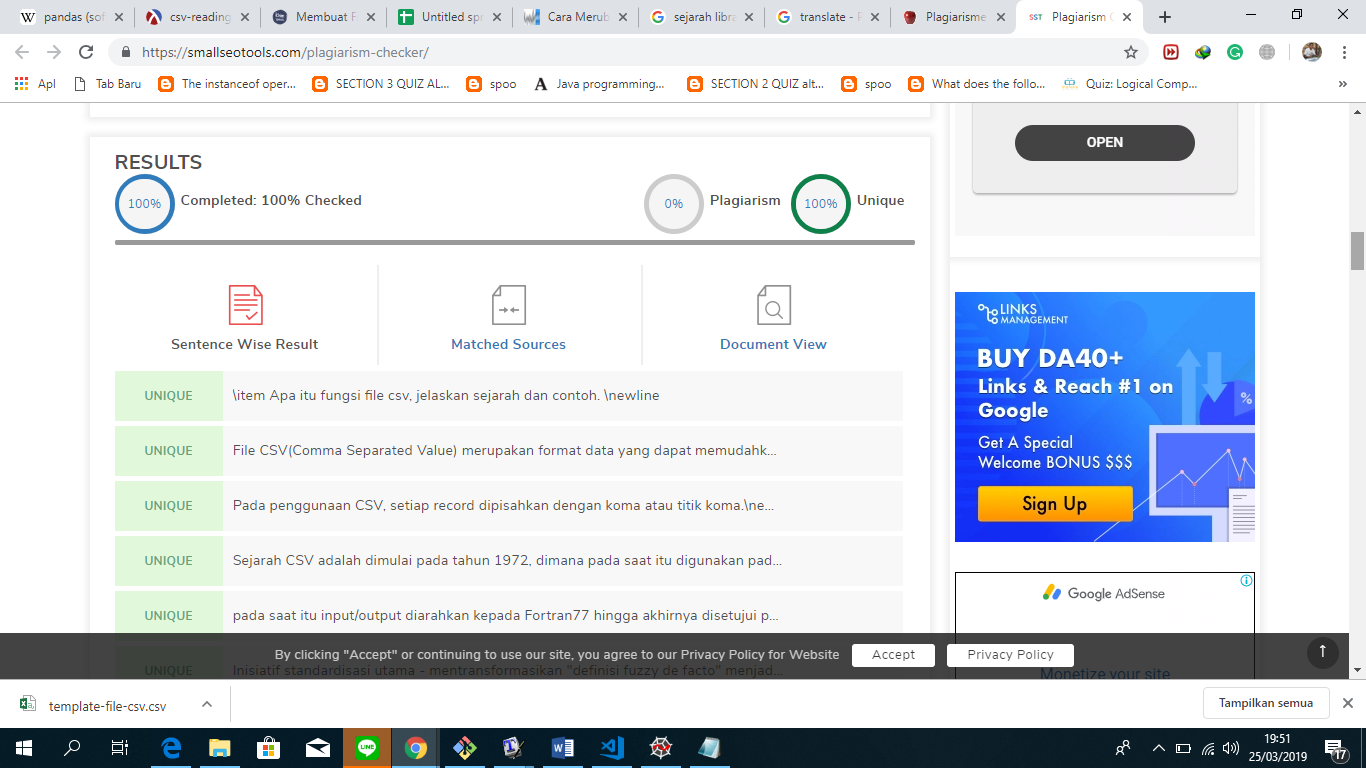
\includegraphics[width=9cm,height=6cm]{figures/nico/Chapter4/plagiarisme.png}
	\caption{Plagiarisme}
	\label{plagiarisme}
\end{figure}
	
\end{enumerate}


%%%%%%%%%%%%%%%%%%%%%%%%%%%%%%%%%%%%%%%%%%%%%%%%%%%%%%%%%%%%%%%%%%%%%%%%%%%%%%%%%%%%%%%%%%%%%%%%%%%%%%%%%%%%%%%%%%%%%%%%%%%%%%%%%%%%%%%%%%%%%%%%%%%%%%%%%%%%%%%%%%%%%%%%%%%%%%%%%%%%%55
\section{Habib Abdul Rasyid}
\subsection{Pemahaman Teori}
\begin {enumerate}
\item Apa itu fungsi file csv, jelaskan sejarah dan contoh Apa itu file CSV ?\newline
File CSV (Comma Separated Values file) adalah jenis file teks biasa yang menggunakan penataan khusus untuk mengatur data 		tabular. Karena ini adalah file teks biasa, ini hanya dapat berisi data teks aktual. dengan kata lain, karakter ASCII atau Unicode 	yang dapat dicetak.\newline
Dari mana File CSV Berasal?\newline
File CSV biasanya dibuat oleh program yang menangani sejumlah besar data. Mereka adalah cara yang nyaman untuk mengekspor data dari spreadsheet dan basis data serta mengimpor atau menggunakannya dalam program lain. Misalnya, Anda dapat mengekspor hasil program penambangan data ke file CSV dan kemudian mengimpornya ke dalam spreadsheet untuk menganalisis data, menghasilkan grafik untuk presentasi, atau menyiapkan laporan untuk publikasi.
File CSV sangat mudah untuk dikerjakan secara terprogram. Bahasa apa pun yang mendukung input file teks dan manipulasi string (seperti Python) dapat bekerja dengan file CSV secara langsung.
Struktur file CSV diberikan oleh namanya. Biasanya, file CSV menggunakan koma untuk memisahkan setiap nilai data tertentu. 
Contoh struktur file CSV :

\begin{figure}[h]
\centering
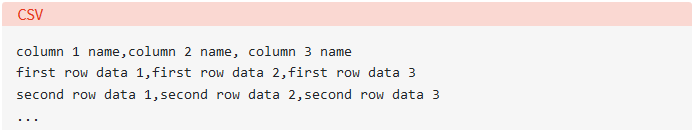
\includegraphics[scale=0.5]{figures/habib/struktur_csv.png}
\caption{Contoh Struktur CSV}
\label{fig:csv}
\end{figure}

\item Aplikasi-aplikasi apa saja yang bisa menciptakan file csv
\begin{itemize}
	\item Texteditor
	Seperti Atom, VS code,sublime dan lain lan.
	\item Program Spreadsheet
	Seperti excel,google spreadshare,LibreOffice, Notepad
	\item Ekspor kontak dari program
	Saat mengekspor kontak dari program lain, misalnya dari Google Mail, Biasanya dapat memilih salah satu dari beberapa format.
	Gmail akan menampilkan pilihan untuk file Google CSV, file Outlook CSV, atau vCard.
\end{itemize}
\item Jelaskan bagaimana cara menulis dan membaca file csv di excel atau spreadsheet\newline
Menulis file csv di excel dan spreadsheet hampir sama yang mana pada bagian header kolom adalah sebagai pembeda dengan data lain.
sehingga baris kedua atau isi dari kolom itu adalah golongan data yang dimasukkan.
untuk membaca file CSV nya dapat menggunakan phyton, berikut adalah code untuk membaca file CSV.\newline
Isi file CSV nya adalah \newline
name,department,birthday month \newline
Habib Abdul Rasyid,Informatics Engineering,Juni \newline
Code untuk memanggilnya 
\lstinputlisting[firstline=7, lastline=20]{src/1174002/1174002_csv.py}
hasilnya

\begin{figure}[h]
\centering
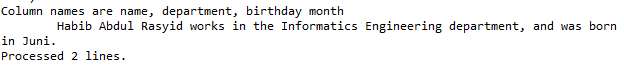
\includegraphics[scale=0.5]{figures/habib/hasil1.png}
\caption{hasil 1}
\label{fig:csv}
\end{figure}

\item Jelaskan sejarah library csv\newline 
Library csv menyediakan fungsionalitas untuk membaca dan menulis ke file CSV. Dirancang untuk bekerja di luar kotak dengan file CSV yang dihasilkan Excel, mudah disesuaikan untuk bekerja dengan berbagai format CSV. Library csv berisi objek dan kode lain untuk membaca, menulis, dan memproses data dari dan ke file CSV.
\item Jelaskan sejarah library pandas\newline 
pandas adalah Library Python open-source yang menyediakan alat analisis data kinerja tinggi dan struktur data yang mudah digunakan. pandas tersedia untuk semua instalasi Python, tetapi itu merupakan bagian penting dari distribusi Anaconda dan bekerja sangat baik di notebook Jupyter untuk berbagi data, kode, hasil analisis, visualisasi, dan teks naratif.
\item Jelaskan fungsi-fungsi yang terdapat di library csv\newline
Fungsi yang terdapat pada library yaitu membaca dan menulis File CSV, Contoh Penulisan Library CSV sama seperti pada Nomor 3 diatas.
Isi file CSV nya adalah \newline
name,department,birthday month\newline
Habib Abdul Rasyid,Informatics Engineering,Juni\newline
Code untuk memanggilnya \newline
\lstinputlisting[firstline=7, lastline=20]{src/1174002/1174002_csv.py}
	\item Jelaskan fungsi-fungsi yang terdapat di library pandas
Fungsi nya sama seperti Library CSV yaitu menulis dan membaca File CSV yang membedakan adalah struktur didalam file nya
berikut ini adalah contohnya.\newline
Isi file CSV nya adalah\newline
Name,Hire Date,Salary,Sick Days remaining\newline
Graham Chapman,03/15/14,50000.00,10\newline
John Cleese,06/01/15,65000.00,8\newline
Eric Idle,05/12/14,45000.00,10\newline
Terry Jones,11/01/13,70000.00,3\newline
Terry Gilliam,08/12/14,48000.00,7\newline
Michael Palin,05/23/13,66000.00,8\newline

Code untuk membacanya.
\lstinputlisting[firstline=21, lastline=24]{src/1174002/1174002_csv.py}
hasilnya
\begin{figure}[h]
\centering
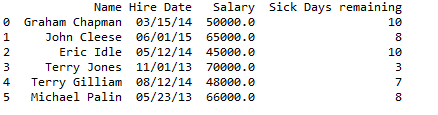
\includegraphics[scale=0.5]{figures/habib/hasil2.png}
\caption{hasil 2}
\label{fig:csv}
\end{figure}

Plagiarisme
\begin{figure}[h]
\centering
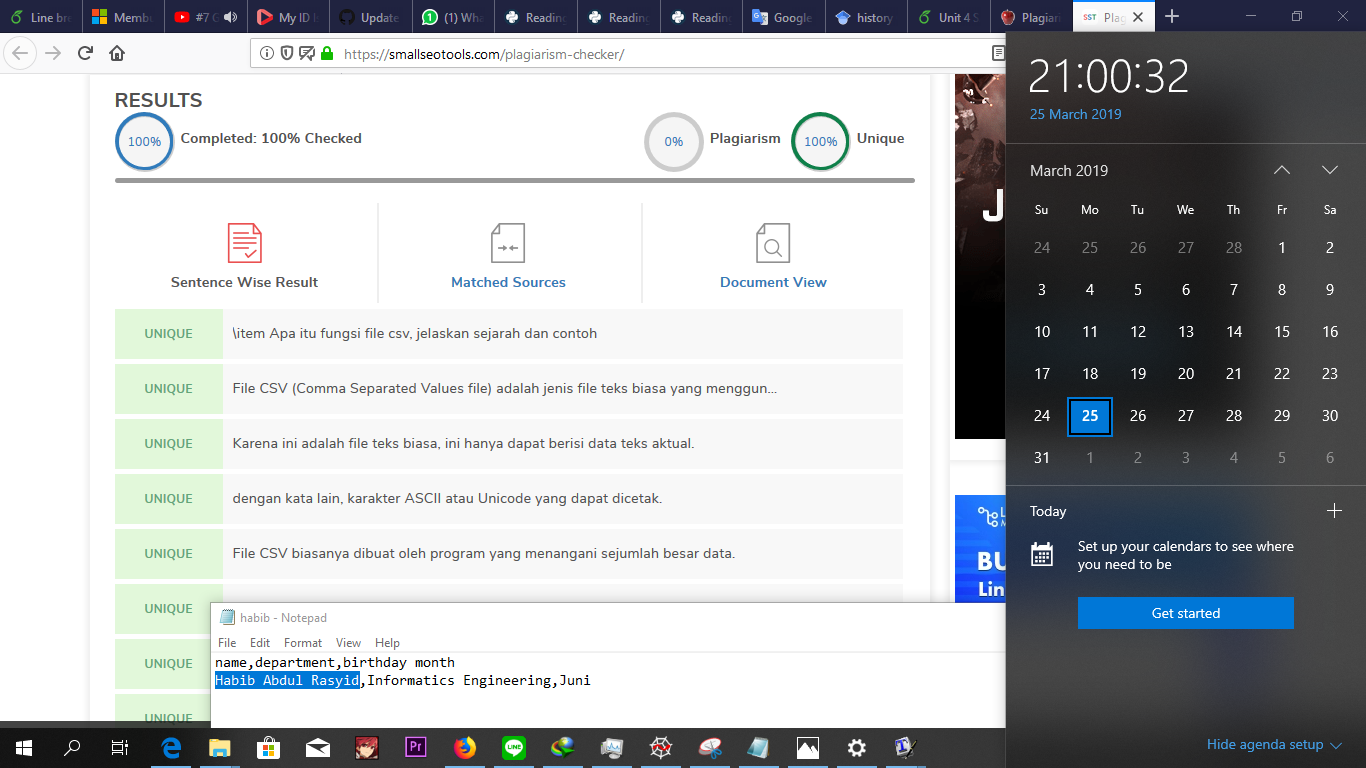
\includegraphics[scale=0.2]{figures/plagiarism_habib.png}
\caption{Bukti Plagiarisme Habib}
\label{fig:plagiarisme}
\end{figure}
\end{enumerate}
%%%%%%%%%%%%%%%%%%%%%%%%%%%%%%%%%%%%%%%%%%%%%%%%%%%%%%%%%%%%%%


\section{Kadek Diva Krishna Murti}

\begin{enumerate}
	\item 
	\textbf{Pengenalan CSV}
	
	Comma Separated Values (CSV) adalah suatu format data yang di mana setiap bagian data dipisahkan dengan tanda koma (,). Format CSV biasanya berfungsi untuk menukar atau mengonversi data ke format lainnya \cite{shafranovich2005common}.
	
	\textbf{Sejarah Format CSV}
	
	IBM Fortran (level H extended) compiler di bawah OS/360 mendukung format CSV pada tahun 1972. FORTRAN 77 mendefinisakan penulisannya dimana input atau output penulisannya menggunakan tanda koma atau spasi untuk pembatas antar data dan penulisan tersebut telah disetujui pada tahun 1978.
	
	Osborne Executive computer yang mengembangkan SuperCalc spreadsheet pada tahun 1983 membuat konvensi kutipan CSV yang memungkinkan string mengandung koma. 
	
	Inisiatif standardisasi utama - mentransformasikan "definisi fuzzy de facto" menjadi definisi yang lebih tepat dan de jure - adalah pada tahun 2005, dengan RFC4180, mendefinisikan CSV sebagai Tipe Konten MIME. Kemudian, pada 2013, beberapa kekurangan RFC4180 ditangani oleh rekomendasi W3C.
	
	Pada 2014 IETF menerbitkan RFC7111 yang menjelaskan aplikasi fragmen URI pada dokumen CSV. RFC7111 menentukan bagaimana rentang baris, kolom, dan sel dapat dipilih dari dokumen CSV menggunakan indeks posisi.
	
	Pada 2015 W3C, dalam upaya meningkatkan CSV dengan semantik formal, mempublikasikan draft rekomendasi pertama untuk standar metadata CSV, yang dimulai sebagai rekomendasi pada bulan Desember tahun yang sama.
	
	\textbf{Contoh penggunaan format CSV}
	
	\lstinputlisting[caption = Contoh penggunaan format CSV., firstline=1, lastline=3]{src/1174006/Chapter4/teori.csv}
	
	\item Aplikasi-aplikasi yang dapat menciptkan file csv, yaitu:
	\begin{enumerate}
		\item Editor teks (Notepad, Sublime, Atom, dan lain-lain)
		\item Spreadsheet (Microsoft Excel dan lain-lain)
	\end{enumerate}
	
	\item Cara menulis dan membaca file csv di excel atau spreadsheet, sebagai berikut:
	
	\textbf{Menulis File CSV}
	
	\begin{enumerate}
		\item Pertama silahkan buka aplikasi Excel dengan cara klik ''Start'', cari Excel, kemudian tekan Enter.
		
		\begin{figure}[H]
			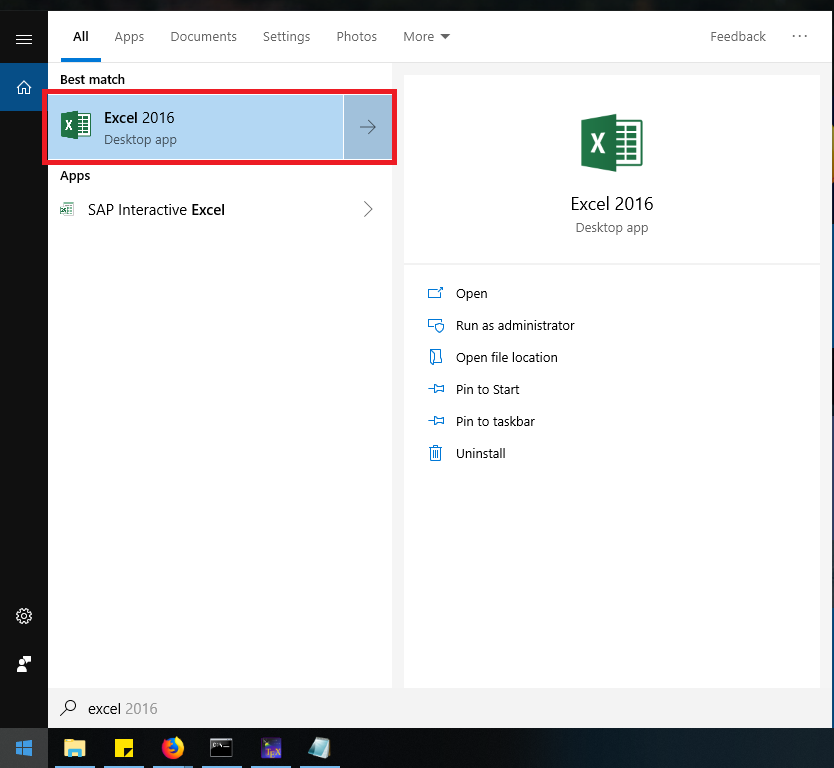
\includegraphics[width=9cm]{figures/diva/Chapter4/t1.png}
			\centering
		\end{figure}
		
		\item Setelah aplikasi terbuka silahkan klik ''Blank Workbook''.
		
		\begin{figure}[H]
			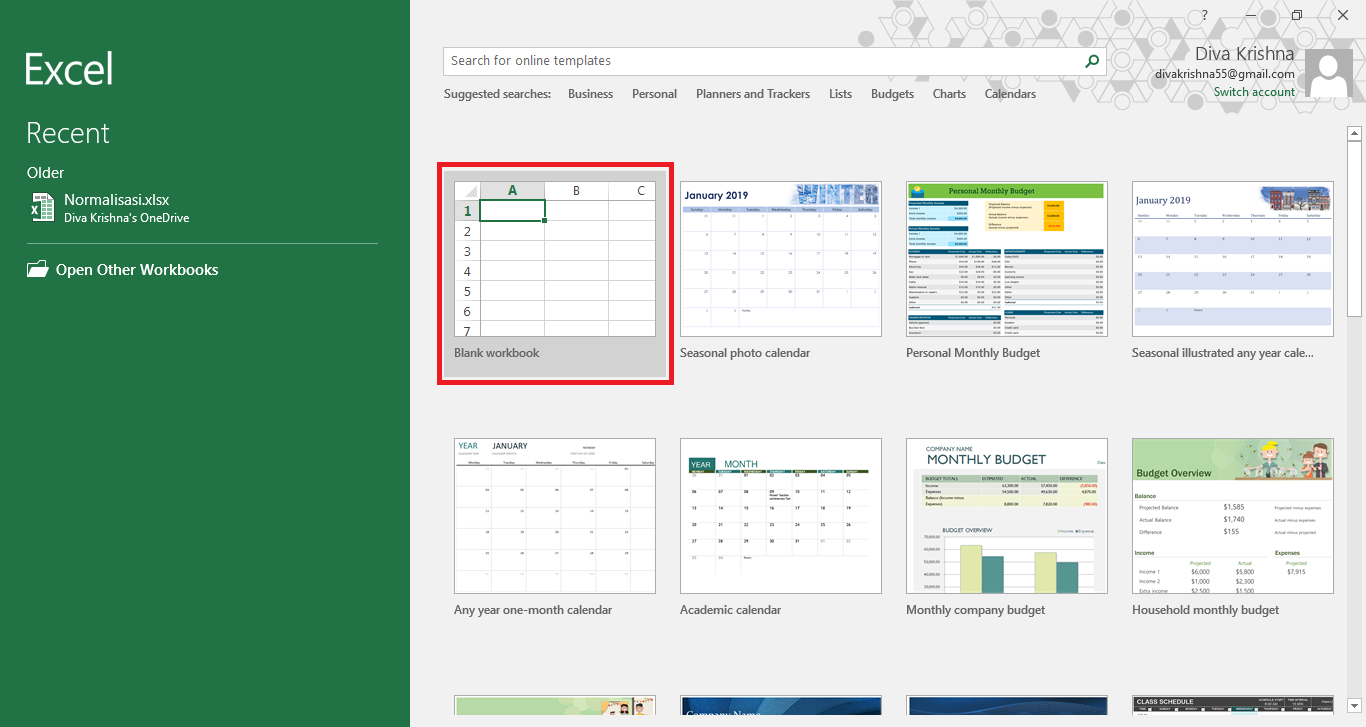
\includegraphics[width=10cm]{figures/diva/Chapter4/t2.png}
			\centering
		\end{figure}
		
		\item Kemudian isi sesuai dengan data yang ingin dibuat.
		
		\begin{figure}[H]
			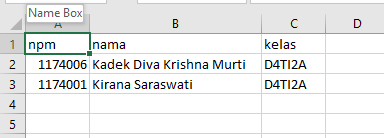
\includegraphics[width=10cm]{figures/diva/Chapter4/t3.png}
			\centering
		\end{figure}
		
		\item Setelah selesai dibuat, silahkan simpan file tersebut dengan cara mengklik ''File'', lalu klik ''Save''.
		
		\begin{figure}[H]
			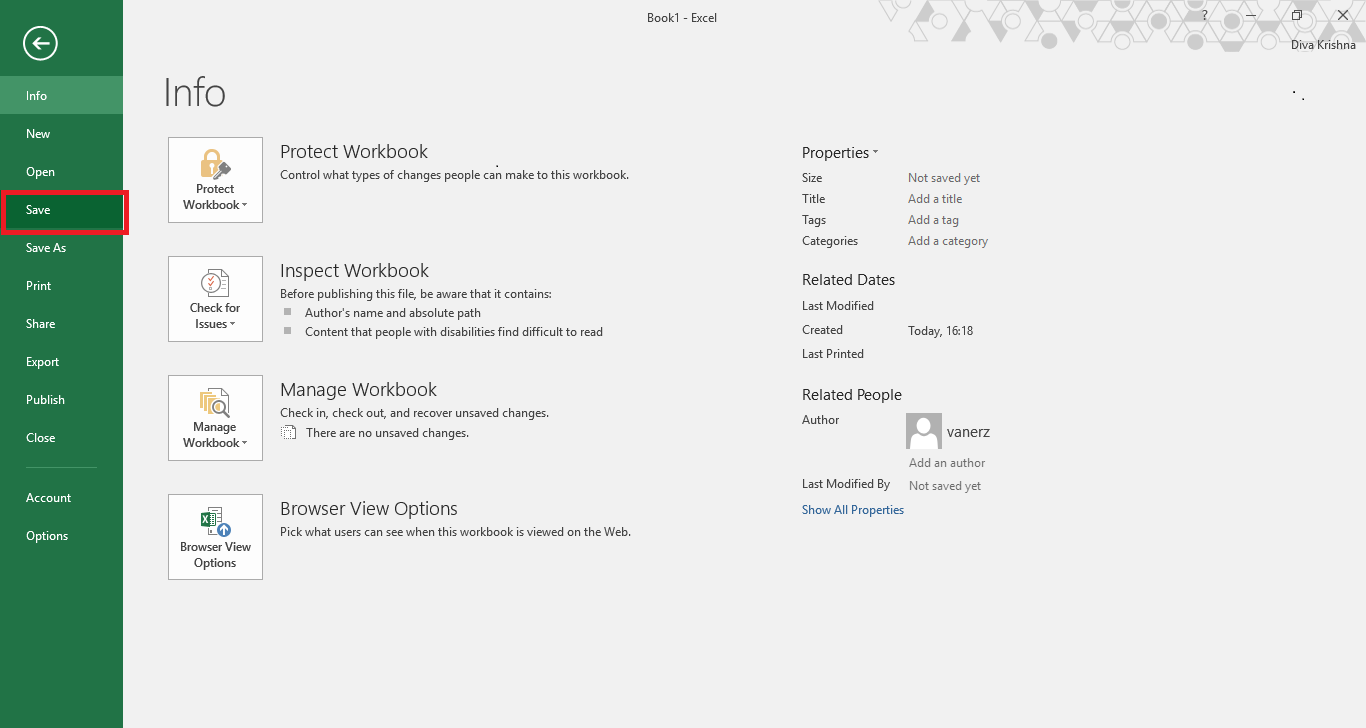
\includegraphics[width=10cm]{figures/diva/Chapter4/t4.png}
			\centering
		\end{figure}
		
		\item Kemudian isi kolom ''File name'' dengan nama file anda dan kolom ''Save as type'' pilih yang berekstensi .csv.
		
		\begin{figure}[H]
			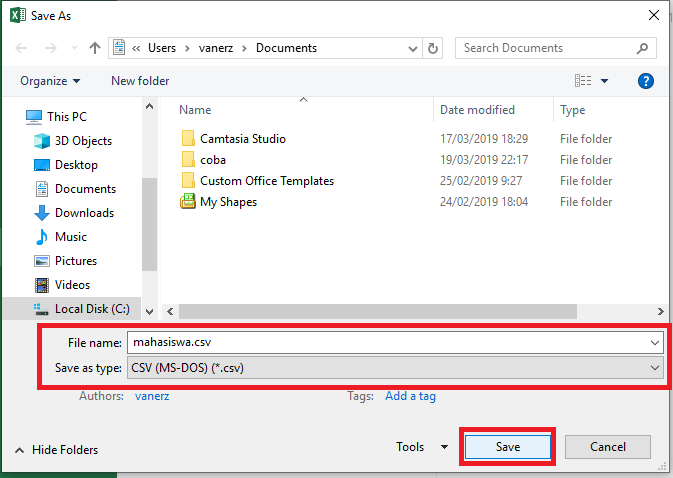
\includegraphics[width=9cm]{figures/diva/Chapter4/t5.png}
			\centering
		\end{figure}
		
		\item Lalu tinggal klik ''Yes''.
		
		\begin{figure}[H]
			\includegraphics[width=7cm]{figures/diva/Chapter4/t6.png}
			\centering
		\end{figure}
		
		\item Kemudian file yang Anda telah terbuat tadi tersimpan dengan ekstensi .csv. Untuk melihat isi filenya tinggal klik dua kali pada file tersebut.
		
		\begin{figure}[H]
			\includegraphics[width=10cm]{figures/diva/Chapter4/t8.png}
			\centering
		\end{figure}
		
		\item Berikut ini adalah isi dari file yang tadi Anda buat.
		
		\begin{figure}[H]
			\includegraphics[width=8cm]{figures/diva/Chapter4/t7.png}
			\centering
		\end{figure}
	\end{enumerate}
	
	\textbf{Melihat File CSV di Excel atau Spreadsheet}
	
	\begin{enumerate}
		\item Pertama klik dua kali pada file yang yang berekstensi CSV.
		
		\begin{figure}[H]
			\includegraphics[width=10cm]{figures/diva/Chapter4/t8.png}
			\centering
		\end{figure}
		
		\item Kemudian file akan terbuka secara otomatis di aplikasi Excel atau spreadsheet.
		
		\begin{figure}[H]
			\includegraphics[width=10cm]{figures/diva/Chapter4/t9.png}
			\centering
		\end{figure}
	\end{enumerate}
	
	\item Sejarah library csv
	
	Library csv mengimplementasikan kelas untuk membaca dan menulis data tabular dalam format CSV. Hal ini memungkinkan programmer untuk mengatakan, "tulis data ini dalam format yang disukai oleh Excel," atau "baca data dari file ini yang dihasilkan oleh Excel," tanpa mengetahui detail yang tepat dari format CSV yang digunakan oleh Excel. Pemrogram juga dapat menggambarkan format CSV yang dipahami oleh aplikasi lain atau menentukan format CSV tujuan khusus mereka sendiri.
	
	\item Sejarah library pandas
	
	Pada 2008, pengembangan pandas dimulai di AQR Capital Management. Pada akhir 2009 telah menjadi open source, dan secara aktif didukung hari ini oleh komunitas individu yang berpikiran sama di seluruh dunia yang menyumbangkan waktu dan energi berharga mereka untuk membantu membuat panda open source menjadi mungkin.
	
	Sejak 2015, pandas adalah proyek yang disponsori NumFOCUS. Ini akan membantu memastikan keberhasilan pengembangan panda sebagai proyek sumber terbuka kelas dunia.
	
	\item Fungsi-fungsi yang terdapat di library csv, yaitu:
	\begin{enumerate}
		\item reader
		
		Fungsi ini digunakan untuk membaca isi file berformat CSV dari list.
		
		\lstinputlisting[caption = Membaca file berformat CSV list., firstline=7, lastline=13]{src/1174006/Chapter4/1174006.py}
		
		\item DictReader
		
		Fungsi ini digunakan untuk membaca isi file berformat CSV dari dictionary.
		
		\lstinputlisting[caption =  Membaca file berformat CSV dictionary., firstline=15, lastline=21]{src/1174006/Chapter4/1174006.py}
		
		\item write
		
		Fungsi ini digunakan untuk menulis file berformat CSV dari list.
		
		\lstinputlisting[caption =  Menulis file berformat CSV list., firstline=23, lastline=30]{src/1174006/Chapter4/1174006.py}
		
		\item DictWrite
		
		Fungsi ini digunakan untuk menulis file berformat CSV dari dictionary.
		
		\lstinputlisting[caption =  Menulis file berformat CSV dictionary., firstline=32, lastline=41]{src/1174006/Chapter4/1174006.py}
		
	\end{enumerate}
	
	\item Fungsi-fungsi yang terdapat di library pandas, yaitu:
	\begin{enumerate}
		\item read\_csv
		
		Fungsi ini digunakan untuk membaca isi file berformat CSV
		
		\lstinputlisting[caption =  Membaca file berformat CSV pandas., firstline=43, lastline=47]{src/1174006/Chapter4/1174006.py}
		
		\item to\_csv
		
		Fungsi ini digunakan untuk menulis file berformat CSV
		
		\lstinputlisting[caption =  Menulis file berformat CSV pandas., firstline=49, lastline=53]{src/1174006/Chapter4/1174006.py}
		
	\end{enumerate}
\end{enumerate}

\textbf{Cek Plagiat Teori}

\begin{figure}[H]
	\includegraphics[width=10cm]{figures/diva/Chapter4/plagiat_teori.png}
	\centering
\end{figure}

\textbf{Kode pada Teori}

\begin{figure}[H]
	\includegraphics[width=10cm]{figures/diva/Chapter4/kode_teori1.png}
	\centering
\end{figure}

\begin{figure}[H]
	\includegraphics[width=10cm]{figures/diva/Chapter4/kode_teori2.png}
	\centering
\end{figure}
%%%%%%%%%%%%%%%%%%%%%%%%%%%%%%%%%%%%%%%%%

\section{Arjun Yuda Firwanda}

\begin{enumerate}
\item Fungsi File CSV, Sejarah dan Contoh
\begin{itemize}
    \item Fungsi CSV (Comma Separated Values) merupakan format file dalam bahasa pemrogaraman python. CSV adalah file yang berextensi.
    \item File CSV merupakan file khusus yang dapat menyimpan informasi di dalam kolom. CSV memudahkan untuk memindahkan dari satu program ke program y .  Ketika teks dan angka disimpan dalam file CSV, mudah untuk memindahkannya dari satu program ke program lainnya. 
    \item Contoh CSV, Microsoft Exel menggunakan format binner atau Binnary Interchange (BIIF). Microsoft merilis office system 2007 dengan format xml. Microsoft Exel juga mendukung format CSV, Dbase File (DBF), Symbolic Link (SYLK), Format Interchange Data (DIF).
\end{itemize}

\item Aplikasi apa saja yang dapat menciptakan file csv
\begin{itemize}
    \item Text Editor seperti Notepad++, Sublime, Visual Studio Code, Atom.
    \item Program Spreedsheet seperti, Microsoft Exel, Google Spreadshare, LibreOffice.
\end{itemize}

\item Cara Menulis dan membaca file CSV di Exel atau Spreadsheet
Cara menulisnya paling atassebagai headernya, untuk mepermudah membedakan data. Baris kedua dan seterusnya itu untuk data itu sendiri. Setelah dibuat kemudian di save as dan pilih format CSV. Dan untuk membuka file yang telah dibuat cukup double klik.

\item Jelaskan Library CSV
Library CSV dibuat untuk memudahkan mengolah data dan mempermudah untuk melakukan export dan import file csv.

\item Jelaskan Library Pandas
Library Pandas dibuat agar bahasa pemograman python bisa bersaing R dan matlab, yang digunakan untuk mengolah banyak data , keperluan big data, data mining data science.

\item Jelaskan fungsi-fungsi yang terdapat pada library CSV
\begin{itemize}
    \item Membaca File, fungsi pembacaan file output yang berupa list sebagai hasilnya.
    \item Menulis File, fungsi menulis file pada csv utnuk menyederhanakan contoh data mahasiswa yang terdiri field yaitu nama, npm, kelas. Dan menyimpan hasilnya dengan format datamhs.csv. Kolom atas sebagai headernya, dan kolom kedua dan seterusnya sebagai datanya.
\end{itemize}

\item Jelaskan fungsi-fungsi yang terdapat pada library Pandas
Fungsi pada library pandas juga hampir sama dengan library csv. Perbedaanya ialah library pandas penulisannya lebih sederhana dan lebih rapih.

\end{enumerate}

%%%%%%%%%%%%%%%%%%%%%%%%%%%%%%%%%%%%%%%%%%%%%%%%%%%%%%%%

\section{Damara benedikta}
\subsection{Pemahaman Materi}
\begin{enumerate}
\item Apa itu fungsi file csv, jelaskan sejarah dan contoh
\paragraph{} CSV (Comma Separated Value) adalah format basis data sederhana yang dimana setiap record yang ada dipisahkan dengan tanda koma (,) atau titik koma (;). Format data file csv dapat diolah dengan berbagai text editor dengan mudah. Anda tidak perlu (dan Anda tidak akan) membuat pengurai CSV Anda sendiri dari awal. Ada beberapa perpustakaan yang dapat diterima yang dapat Anda gunakan. Pustaka csv Python akan berfungsi untuk sebagian besar kasus. Jika pekerjaan Anda memerlukan banyak data atau analisis numerik, panda library juga memiliki kemampuan penguraian CSV, yang seharusnya menangani sisanya. Dalam bahasa pemrograman Python telah disediakan modul csv yang khusus untuk mengolah data berformat csv.  Untuk memanipulasi data csv dengan python tentunya yang pertama dilakukan adalah mengimport modul csv dengan perintah import csv. File CSV biasanya dibuat oleh program yang menangani sejumlah besar data. Mereka adalah cara yang nyaman untuk mengekspor data dari spreadsheet dan basis data serta mengimpor atau menggunakannya dalam program lain. Misalnya, Anda dapat mengekspor hasil program penambangan data ke file CSV dan kemudian mengimpornya ke dalam spreadsheet untuk menganalisis data, menghasilkan grafik untuk presentasi, atau menyiapkan laporan untuk publikasi. Contoh nya adalah sebagai berikut :

 \lstinputlisting[firstline=8, lastline=20]{src/1174012/csvako.py}

\item Aplikasi-aplikasi apa saja yang bisa menciptakan file csv?
\paragraph{} Ada beberapa aplikasi yang dapat menciptakan file dengan format csv diantaranya google sheet, number di MacOS dan microsoft excel.
\subsection{Membuat dan membaca csv di excel atau spreadsheet}

\item Jelaskan bagaimana cara menulis dan membaca file csv di excel atau spreadsheet
\paragraph{} Cara membuat file csv di excel cukup mudah yaitu :
\begin{itemize}
	\item Buat foldernya
	\item Pilih save as
	\item pilih file dengan format csv
\end{itemize}
Cara membaca file di csv :
\begin{itemize}
	\item Klik data - get external data - form text
	\item Akan muncul Text Import Wizard, arahkan pada file csv yang ingin anda buka lalu Open.
	\item Setelah File terbuka, akan muncul Text Import Wizard.
	\item Pilih Delimited, Kemudian Next (Di sini, bisa juga menentukan baris awal yang akan di import)
	\item Centrang pada Tab dan Comma (Atau sesuai pengaturan File Anda) lalu Next.
	\item Atur Format data pada tiap kolom yang tampil dan klik Finish
\end{itemize}

\item Jelaskan sejarah library csv
\paragraph{} CSV muncul untuk memudahkan data science dan analis karena dinilai terdapat banyak kemudahan yang didapat. CSV dapat dimaksimalkan jika dipaduka dengan python karena python adalah bahasa pemrograman yang support ke banyak library termasuk csv. Maka karena itulah perpaduan python dan csv seringkali digunakan oleh perusahaan-perushaan besar dalam mengolah datanya.

\item Jelaskan sejarah library pandas
\paragraph{} Pandas merupakan tool yang dapat digunakan sebagai alat analisis data dan struktur untuk bahasa pemrograman Python. Pandas dapat mengolah data dengan mudah, salah satu fitur yang ada dalam pandas adalah Dataframe. Fitur dataframe dapat membaca sebuah file dan menjadikannya tabble, juga dapat mengolah suatu data dengan menggunakan operasi seperti join, group by dan teknik lainnya yang terdapat pada SQL. Dalam hal ini pandas tidak jauh beda dengan csv yaitu memiliki keunggulan dalam pengolahan data-data besar dan dapat disupport dengan baik dengan python walaupun mengimport data dalam jumlah banyak.

\item Jelaskan fungsi-fungsi yang terdapat di library csv
\paragraph{} Library csv mempunyai keunggulan dibandingkan format data lainnya adalah soal kompatibilitas. File csv dapat digunakan, diolah, diekspor/impor, dan dimodifikasi menggunakan berbagai macam perangkat lunak dan bahasa pemrograman. Pada library csv mempunyai fungsi import dan eksport data yang baik dan bisa digunakan dalam jumlah besar.

\item Jelaskan fungsi-fungsi yang terdapat di library pandas
\paragraph{} pandas menyediakan beragam fungsi operasi untuk mengolah data. Contoh jika menggunakan series bisa mencari nilai max, min, dan mean secara langsung, bahkan juga bisa melakukan operasi perpangkatan pada nilai Series secara langsung.
Pandas dapat mengolah suatu data dan mengolahnya seperti join, distinct, group by, agregasi, dan teknik seperti pada SQL. Hanya saja dilakukan pada tabel yang dimuat dari file ke RAM.
\end{enumerate}


%%%%%%%%%%%%%%%%%%%%%%%%%%%%%%%%%%%%%%

\section{Muh. Rifky Prananda}
\begin{enumerate}
       \item Apa itu fungsi file csv, jelaskan sejarah dan contoh
       file csv atau nilai terbatas koma adalah suatu jenis file terkhusus yang bisa diedit atau dibuat di excel. file csv sendiri menyimpan sebuah informasi yang terpisahkan oleh koma, dan tidak menyimpan informasi didalam kolom.ketika angka dan teks disimpan didalam file csv, angka dan teks tersebut mudah untuk dipindahkan dari satu program ke program yang lain.
Dari rilis pertama, Excel menggunakan format file biner yang disebut Binary Interchange File Format (BIFF) sebagai format file utamanya. Ini berubah ketika Microsoft merilis Office System 2007 yang memperkenalkan Office Open XML sebagai format file utamanya. Office Open XML adalah file kontainer berbasis XML yang mirip dengan XML Spreadsheets (XMLSS), yang diperkenalkan di Excel 2002. File versi XML tidak bisa menyimpan makro VBA.Meskipun mendukung format XML baru, Excel 2007 masih mendukung format lama yang masih berbasis pada BIFF tradisional. Selain dari yang di atas, Microsoft Excel juga dapat mendukung Comma Separated Values (CSV), DBase Files (DBF), format Data Interchange Data (DIF) dan banyak format lainnya, termasuk lembar kerja 1-2 Lotus- 3 (WKS, WK1, WK2, dll.) Dan Quattro Pro.
        \item aplikasi-aplikasi apa saja yang bisa menciptakan file csv 
        \begin{itemize}
               \item Program spredsheet
               contohnya seperti google spreadsheet, excel, libreOfficecalc
               \item texteditor
               contohnya seperti sublime, atom, notepad++, visual studio code, dan lain sebagainya.
        \end{itemize}
        \item jelaskan bagaimana cara menulis dan membaca file csv di excel atau spreadsheet 
        untuk bisa menuliskannya dan dibagian paling atas itu dibuat headernya, untuk lebih mempermudah membedakan datanya, dan untuk baris selanjutnya atau kedua dan seterusnya itu untuk datanya itu sendiri. setelah itu, pilih save as dan pilih format csv. dan untuk membukanya bisa di klik dua kali di file tersebut.
        \item jelaskan sejarah library csv
        library csv sengaja dibuat untuk memudahkan dalam proses pengelolaan data. dan dapat mempermudah untuk melakukan import dan eksport file csv itu sendiri. 
        \item jelaskan sejarah library pandas
        library pandas sengaja dibuat untuk bahasa pemrograman python agar bisa bersaing matlab dan R, yang dapat digunakan untuk mengelola banyak data, keperluan big data, data mining, data sciense dan sebagainya. 
        \item jelaskan fungsi-fungsi yang terdapat di library csv
        didalam library csv terdapat 2 fungsi yang bisa digunakan olehnya:
        pertama yaitu fungsi yang bisa membaca sebuah file csv.
        kedua yaitu fungsi yang bisa menulis sebuah file csv.
        \item jelaskan fungsi-fungsi yang terdapat di library pandas
        yang pertama yaitu fungsi yang disebut tail dan head yang digunakan untuk melihat sampel data.
        yang kedua yaitu fungsi add yang biasa digunakan untuk menambahkan data. 
\end{enumerate}

%%%%%%%%%%%%%%%%%%%%%%%%%%%%%%%%%%%%%%%%%%%%%%%%%%%%%%%%
\section{Oniwaldus Bere Mali}
\begin{enumerate}
\item Fungsi file csv,sejarah dan contoh :
File CSV (Comma Limited Value) adalah jenis file khusus yang dapat Anda buat atau edit di Excel. File CSV menyimpan informasi yang dipisahkan oleh koma, tidak menyimpan informasi dalam kolom. Ketika teks dan angka disimpan dalam file CSV, mudah untuk memindahkannya dari satu program ke program lainnya.
Dari rilis pertama, Excel menggunakan format file biner yang disebut Binary Interchange File Format (BIFF) sebagai format file utamanya. Ini berubah ketika Microsoft merilis Office System 2007 yang memperkenalkan Office Open XML sebagai format file utamanya. Office Open XML adalah file kontainer berbasis XML yang mirip dengan XML Spreadsheets (XMLSS), yang diperkenalkan di Excel 2002. File versi XML tidak bisa menyimpan makro VBA.
Meskipun mendukung format XML baru, Excel 2007 masih mendukung format lama yang masih berbasis BIFF tradisional. Selain itu Microsoft Excel juga mendukung format Comma Separated Values (CSV), DBase File (DBF), SYMbolic LinK (SYLK), Format Interchange Data (DIF) dan banyak format lainnya, termasuk format lembar kerja 1-2 Lotus - 3 (WKS, WK1, WK2, dll.) Dan Quattro Pro.
\item Aplikasi yang  bisa menciptakan file csv :
\begin{itemize}
\item Texteditor
Seperti notepad++,visual studio code,atom,sublime,notepad dan lain sebagainya
\end{itemize}
\item Cara menulis dan membaca file csv di excel atau spreadsheet :
Untuk menulisnya untuk yang paling atas itu kita buat headernya,untuk mepermudah membedakan datanya,dan untuk baris kedua dan seterusnya itu untuk data itu sendiri.
dan setelah di buat kalian save as kemudian pilih format CSV.
dan untuk membukan cukup di double clik file tersebut
\item Sejarah library csv:
library csv dibuat untuk permudah mengolah data. Dan mempermudah untuk melakukan export dan import file csv itu sendiri
\item Sejarah library pandas dari :
library pandas dibuat agar bahasa pemograman python bisa bersaing R dan matlab, yang digunakan untuk mengolah banyak data , keperluan big data, data mining data science dan sebagainya.
\item Fungsi-fungsi yang terdapat di library csv :
Dalam librarycsv terdapat 2 fungsi yang bisa digunakan oleh library csv
Pertama,fungsi membaca file csv.
fungsi ini bisa menggunakan list dan dictionarys
 \item Fungsi-fungsi yang terdapat di library pandas :
    Hampir sama dengan library csv,tp library pandas penulisannya lebih sederhana dan terlihat lebih rapih dari pada library csv.

\subsection{Cek Plagiarisme}
\begin{figure}[!htbp]
\centering
\includegraphics[width=3cm,height=3cm]{figures/oni/plagiat.PNG}
\caption{Plagiarisme}
\label{plagiarisme}\end{figure}
\end{enumerate}


\chapter{Kelompok 2}
\section{Rahmatul Ridha}
\subsection{Pemahaman Teori}
Kerjakan soal berikut ini, masing-masing bernilai 5 untuk hari pertama. Praktek teori penungjang yang dikerjakan dengan deadline besok jam 4 pagi :
\begin{enumerate}
 \item Apa itu fungsi file csv, jelaskan sejarah dan contohnya.
   \begin{itemize}
    \item Apa itu Fungsi file csv
     Format file csv \textit{Comma Separated Values} yaitu suatu format data pada basis data dimana setiap record yang dapat dipisahkan dengan menggunakan tanda koma (`,’) atau juga bisa dengan menggunakan titik koma (`;’) sebagai tanda pemisah antara datu elemen dengan elemen yang lainnya. Selain bahasa programnya yang sederhana, format ini juga dapat dibuka dengan menggunakan berbagai \textit{text-editor} seperti Notepad, Wordpad, dan MS Excel.

     File CSV (nilai berbatas koma) merupakan tipa file khusus yang dapat dibuat atau diedit dengan menggunakan excel. File csv menyimpan informasi yang dapat dipisah oleh koma (,), bukan untuk menyimpan informasi dalam kolom. Saat teks dan angka yang disimpan dalam file csv, dapat memudahkan untuk memindahkannya dari satu program ke program yang lainnya.

    \item Sejarah CSV

     Nilai yang dipisahkan oleh koma adalah format data yang memberi tanggal lebih awal pada komputer pribadi lebih dari satu dekade: kompiler IBM Fortran (level H extended) di bawah OS / 360 mendukungnya pada tahun 1972. Input / output yang diarahkan oleh daftar ("bentuk bebas") didefinisikan dalam FORTRAN 77, disetujui pada tahun 1978. Input yang diarahkan daftar menggunakan koma atau spasi untuk pembatas, sehingga string karakter yang tidak dikutip tidak dapat mengandung koma atau spasi.

     Nama "nilai yang dipisahkan koma" dan singkatan "CSV" digunakan pada tahun 1983. Manual untuk komputer Osborne Executive, yang menggabungkan SuperCalc spreadsheet, mendokumentasikan konvensi kutipan CSV yang memungkinkan string berisi koma yang disematkan, tetapi manual tersebut tidak menentukan konvensi untuk menyematkan tanda kutip dalam string yang dikutip. Daftar nilai yang dipisahkan koma lebih mudah untuk diketik (misalnya ke dalam kartu berlubang) daripada data yang selaras dengan kolom tetap dan cenderung menghasilkan hasil yang salah jika suatu nilai dilubangi satu kolom dari lokasi yang dituju.

     Pada 2014 IETF menerbitkan RFC7111 yang menjelaskan aplikasi fragmen URI ke dokumen CSV. RFC7111 menentukan bagaimana rentang baris, kolom, dan sel dapat dipilih dari dokumen CSV menggunakan indeks posisi. Pada 2015 W3C, dalam upaya meningkatkan CSV dengan semantik formal, mempublikasikan draft rekomendasi pertama untuk standar metadata CSV, yang dimulai sebagai rekomendasi pada bulan Desember tahun yang sama.

     \item Contohnya
       \lstinputlisting[caption = Contoh penggunaan format CSV., firstline=1, lastline=3]{src/1144124/Chapter4/teori.csv}
     \end{itemize}

 \item Aplikasi-aplikasi apa saja yang bisa menciptakan file csv ?
       \begin{itemize}
         \item Text editor (Notepat, Wordpad, dan lain-lain)
         \item Spreadsheet (Microsoft Excel)
       \end{itemize}

 \item Jelaskan bagaimana cara menulis dan membaca file csv diexcel atau spreadsheet.
    \textbf{Menulis File CSV}
       \begin{enumerate}
	   \item Buat dokumen baru diexcel.
       \item Tambahkan judul kolom untuk setiap potongan informasi yang ingin dicatat, contohnya npm, nama, kelas. Lalu ketikkn informasi delam kolom yang sesuai.
	   \item Setelah selesai dibuat, file excel yang telah dibuat akan terlihat seperti \ref{CSV}
		
		\begin{figure}[H]	\includegraphics[width=10cm]{figures/rahma/Chapter4/1.png}
		\centering
        \label{CSV}
		\end{figure}
		
	   \item Kemudian isi kolom `File name' dengan nama file anda dan kolom `Save as type' pilih yang berekstensi .csv.
		
		\begin{figure}[H] \includegraphics[width=9cm]{figures/rahma/Chapter4/2.png}
			\centering
		\end{figure}

\item Kemudian file yang Anda telah terbuat tadi tersimpan dengan ekstensi .csv. Untuk melihat isi filenya tinggal klik dua kali pada file tersebut.
		\begin{figure}[H]	\includegraphics[width=10cm]{figures/rahma/Chapter4/3.png}
			\centering
		\end{figure}
		
	   \item Lalu tinggal klik `Yes'.	
		\begin{figure}[H] \includegraphics[width=7cm]{figures/rahma/Chapter4/4.png}
			\centering
		\end{figure}


   \textbf{Melihat File CSV di Excel atau Spreadsheet}
	 \begin{enumerate}
		\item Pertama klik dua kali pada file yang yang berekstensi CSV.
		
		\begin{figure}[H]	\includegraphics[width=10cm]{figures/rahma/Chapter4/5.png}
			\centering
		\end{figure}
		
		\item Kemudian file akan terbuka secara otomatis di aplikasi Excel atau spreadsheet.
		
		\begin{figure}[H] \includegraphics[width=10cm]{figures/rahma/Chapter4/6.png}
			\centering
		\end{figure}
	 \end{enumerate}

   \item Jelaskan sejarah library csv.
   Format yang disebut CSV \textit{Comma Separated Values} adalah format impor dan ekspor paling umum untuk spreadsheet dan basis data. Format CSV digunakan selama bertahun-tahun sebelum upaya untuk menggambarkan format dengan cara standar di RFC 4180. Kurangnya standar yang didefinisikan dengan baik berarti bahwa perbedaan halus sering ada dalam data yang diproduksi dan dikonsumsi oleh aplikasi yang berbeda. Perbedaan-perbedaan ini dapat membuatnya menjengkelkan untuk memproses file CSV dari berbagai sumber.

   Namun, sementara pembatas dan mengutip karakter bervariasi, format keseluruhan cukup mirip sehingga dimungkinkan untuk menulis satu modul yang dapat secara efisien memanipulasi data seperti itu, menyembunyikan detail membaca dan menulis data dari programmer. Modul csv mengimplementasikan kelas untuk membaca dan menulis data tabular dalam format CSV.

   Hal ini memungkinkan programmer untuk mengatakan, "tulis data ini dalam format yang disukai oleh Excel," atau "baca data dari file ini yang dihasilkan oleh Excel," tanpa mengetahui detail yang tepat dari format CSV yang digunakan oleh Excel. Pemrogram juga dapat menggambarkan format CSV yang dipahami oleh aplikasi lain atau menentukan format CSV tujuan khusus mereka sendiri.

   \item Jelaskan sejarah library Pandas.
   Pandas merupakan toolkit yang powerfull sebagai alat analisis data dan struktur untuk bahasa pemrograman Python. Dengan menggunakan pandas kita dapat mengolah data dengan mudah, salah satu fiturnya adalah Dataframe. Dengan adanya fitur dataframe kita dapat membaca sebuah file dan menjadikannya tabble, kita juga dapat mengolah suatu data dengan menggunakan operasi seperti join, distinct, group by, agregasi, dan teknik lainnya yang terdapat pada SQL. Banyak format file yang dapat dibaca menggunakan Pandas, seperti file .txt, .csv, .tsv dan lainnya. Agar lebih jelas mari kita mencobanya secara langsung.

   \item Jelaskan fungsi-fungsi yang terdapat dilibrary csv.
       \begin{enumerate}
		\item reader
		
		Fungsi ini digunakan untuk membaca isi file berformat CSV dari list.
		
		\lstinputlisting[caption = Membaca file berformat CSV list., firstline=7, lastline=13]{src/1144124/Chapter4/1144124.py}
		
		\item DictReader
		
		Fungsi ini digunakan untuk membaca isi file berformat CSV dari dictionary.
		
		\lstinputlisting[caption =  Membaca file berformat CSV dictionary., firstline=15, lastline=21]{src/1144124/Chapter4/1144124.py}
		
		\item write
		
		Fungsi ini digunakan untuk menulis file berformat CSV dari list.
		
		\lstinputlisting[caption =  Menulis file berformat CSV list., firstline=23, lastline=30]{src/1144124/Chapter4/1144124.py}
		
		\item DictWrite
		
		Fungsi ini digunakan untuk menulis file berformat CSV dari dictionary.
		
		\lstinputlisting[caption =  Menulis file berformat CSV dictionary., firstline=32, lastline=41]{src/1144124/Chapter4/1144124.py}
		
	\end{enumerate}
   \item Jelaskan fungsi-fungsi yang terdapat di library pandas.
       \begin{enumerate}
		\item read\_csv
		
		Fungsi ini digunakan untuk membaca isi file berformat CSV
		
		\lstinputlisting[caption =  Membaca file berformat CSV pandas., firstline=43, lastline=47]{src/1144124/Chapter4/1144124.py}
		
		\item to\_csv
		
		Fungsi ini digunakan untuk menulis file berformat CSV
		
		\lstinputlisting[caption =  Menulis file berformat CSV pandas., firstline=49, lastline=53]{src/1144124/Chapter4/1144124.py}
		
	\end{enumerate}
   \item Cek plagiarisme
Berikut adalah cek plagiarisme pada teorinya pada \ref{Plagiarisme}
   \begin{figure}[H]
	\includegraphics[width=10cm]{figures/rahma/Chapter4/Plagiarisme.jpg}
	\centering
    \label{Plagiarisme}
    \end{figure}

 \end{enumerate} 

\chapter{Kelompok 3}
\section{Harun Ar - Rasyid}
\subsection{Penangganan error}
dalam praktek kali ini alhamdulliha tidak menemukan error

%%%%%%%%%%%%%%%%%%%%%%%%%%%%%%%%%%%%%%%%%%%%%%%%%%%%%%%%%%%%%

\section{Kadek Diva Krishna Murti}
\begin{enumerate}
	\item Tuliskan  peringatan  error  yang  didapat  dari  mengerjakan  praktek  keempat  ini, dan  jelaskan  cara  penanganan  error  tersebut.   dan  Buatlah  satu  fungsi  yang menggunakan gunakan try except untuk menanggulangi error tersebut.
	
	Peringatan error di praktek keempat ini, yaitu:
	\begin{itemize}
		\item Syntax Errors
		Syntax Errors adalah suatu keadaan saat kode python mengalami kesalahan penulisan. Solusinya adalah memperbaiki penulisan kode yang salah.
		
		\item Name Error
		NameError adalah exception yang terjadi saat kode melakukan eksekusi terhadap local name atau global name yang tidak terdefinisi. Solusinya adalah memastikan variabel atau function yang dipanggil ada atau tidak salah ketik.
		
		\item Type Error
		TypeError adalah exception yang akan terjadi apabila pada saat dilakukannya eksekusi terhadap suatu operasi atau fungsi dengan type object yang tidak sesuai. Solusi dari error ini adalah mengkoversi varibelnya sesuai dengan tipe data yang akan digunakan.
	\end{itemize}
	
	Fungsi yang menggunakan try except
	\lstinputlisting[caption= Fungsi yang menggunakan try except .,firstline=55, lastline=67]{src/1174006/Chapter4/1174006.py}
\end{enumerate}

\textbf{Kode Program}
\begin{figure}[H]
	\includegraphics[width=10cm]{figures/diva/Chapter4/harikedua/p1.png}
	\centering
\end{figure}

\textbf{Cek Plagiat}
\begin{figure}[H]
	\includegraphics[width=10cm]{figures/diva/Chapter4/harikedua/plagiatpenanganan.png}
	\centering
\end{figure}

%%%%%%%%%%%%%%%%%%%%%%%%%%%%%%%%%%%%%%%%%%%%%%%%%%%%%%%%%%%%%%%%%%%%%%%%%%%%%%%%%%%%%%

\bibliographystyle{IEEEtran} 
%\def\bibfont{\normalsize}
%\bibliography{references}


%%%%%%%%%%%%%%%
%%  The default LaTeX Index
%%  Don't need to add any commands before \begin{document}
\printindex

%%%% Making an index
%% 
%% 1. Make index entries, don't leave any spaces so that they
%% will be sorted correctly.
%% 
%% \index{term}
%% \index{term!subterm}
%% \index{term!subterm!subsubterm}
%% 
%% 2. Run LaTeX several times to produce <filename>.idx
%% 
%% 3. On command line, type  makeindx <filename> which
%% will produce <filename>.ind 
%% 
%% 4. Type \printindex to make the index appear in your book.
%% 
%% 5. If you would like to edit <filename>.ind 
%% you may do so. See docs.pdf for more information.
%% 
%%%%%%%%%%%%%%%%%%%%%%%%%%%%%%

%%%%%%%%%%%%%% Making Multiple Indices %%%%%%%%%%%%%%%%
%% 1. 
%% \usepackage{multind}
%% \makeindex{book}
%% \makeindex{authors}
%% \begin{document}
%% 
%% 2.
%% % add index terms to your book, ie,
%% \index{book}{A term to go to the topic index}
%% \index{authors}{Put this author in the author index}
%% 
%% \index{book}{Cows}
%% \index{book}{Cows!Jersey}
%% \index{book}{Cows!Jersey!Brown}
%% 
%% \index{author}{Douglas Adams}
%% \index{author}{Boethius}
%% \index{author}{Mark Twain}
%% 
%% 3. On command line type 
%% makeindex topic 
%% makeindex authors
%% 
%% 4.
%% this is a Wiley command to make the indices print:
%% \multiprintindex{book}{Topic index}
%% \multiprintindex{authors}{Author index}

\end{document}

